\documentclass[
12pt, % The default document font size, options: 10pt, 11pt, 12pt
b5paper,
%draft,
%oneside, % Two side (alternating margins) for binding by default, uncomment to switch to one side
english, % ngerman for German
%singlespacing, % Single line spacing, alternatives: onehalfspacing or doublespacing
%draft, % Uncomment to enable draft mode (no pictures, no links, overfull hboxes indicated)
%nolistspacing, % If the document is onehalfspacing or doublespacing, uncomment this to set spacing in lists to single
%liststotoc, % Uncomment to add the list of figures/tables/etc to the table of contents
%toctotoc, % Uncomment to add the main table of contents to the table of contents
%parskip, % Uncomment to add space between paragraphs
]{book}
%
\usepackage{fancyhdr}
\usepackage{float}
\usepackage{amsmath,amssymb}
\usepackage{amsthm}
\usepackage{thmtools}
\usepackage{mathtools}
\usepackage{mathpartir}
\usepackage[T1]{fontenc} 
\usepackage{textcomp}
\usepackage[table]{xcolor}
\usepackage{stmaryrd}
\usepackage{enumerate}
\usepackage[shortlabels]{enumitem}
\usepackage{amsthm}
\newtheorem{definition}{Definition}[section]
\usepackage{listings}
\usepackage{prooftree}
\usepackage{hyperref}
\hypersetup{
    colorlinks=true,       % false: boxed links; true: colored links
    linkcolor=blue,          % color of internal links
    citecolor=blue,        % color of links to bibliography
    filecolor=blue,      % color of file links
    urlcolor=blue 
}
\usepackage[nottoc,chapter]{tocbibind}
\usepackage{caption}
\usepackage{subcaption}
\usepackage{listings}
\lstset{
  numbers=left,
  stepnumber=1,    
  firstnumber=1,
  numberfirstline=true,
  %xleftmargin=0.5cm,
  basicstyle= \ttfamily
}
\usepackage{babel}
\usepackage{titlesec}
\setcounter{secnumdepth}{3}
\usepackage[final]{pdfpages}
\usepackage{acronym}
\usepackage{geometry}
\usepackage{dirtytalk}
\usepackage{listings}
\usepackage{float}
\usepackage[ruled,vlined,linesnumbered]{algorithm2e}
\usepackage{microtype}
\usepackage{multirow}
\usepackage{upgreek}
%----------------------------------------------------------------------------------------
%	WATERMARK -> COMMENT WHEN FINAL DOCUMENT IS DONE
%----------------------------------------------------------------------------------------
%\usepackage{draftwatermark}
%\SetWatermarkText{Draft}
%\SetWatermarkScale{4}
%\SetWatermarkColor[gray]{0.9}

\RequirePackage{geometry}
\geometry{
	paper=b5paper, % Default paper size, change to "letterpaper" for US Letter (you'll need to adjust margins after)
	inner=1in, % The inner margin (beside binding)
	outer=1in, % The outer margin (opposite binding)
	top=1in, % Top margin
	bottom=1in, % bottom margin
	headsep=.5in, % Header separation
	footnotesep=.5in,
	includehead,
	includefoot
}

\raggedbottom

\setcounter{tocdepth}{3}
\setcounter{secnumdepth}{3}

%----------------------------------------------------------------------------------------
%	PENALTIES
%----------------------------------------------------------------------------------------

\doublehyphendemerits=10000 % No consecutive line hyphens
\brokenpenalty=10000 % No broken words across columns/pages
\widowpenalty=9999 % Almost no widows at bottom of page
\clubpenalty=9999 % Almost no orphans at top of page
\interfootnotelinepenalty=9999 % Almost never break footnotes
%
%
\makeatletter
\def\arcr{\@arraycr}
\makeatother
%
%
\newcommand{\htv}[1]{\marginpar{\tiny\textbf{Hugo}:  #1}}

%Encoding

\newcommand{\encode}[2]{\llbracket #1 \rrbracket_{#2}}
\newcommand{\enc}[1]{\llbracket #1 \rrbracket}
\newcommand{\handler}{\mathit{H}}



% Macros from Hugo's sources
\newcommand{\der}                             	{\vdash}
\newcommand{\wf}{\der}
\newcommand\BEND{{\mathbf{end} } }
\newcommand{\apart} 				{\#}
\newcommand\PAR{\hspace{0.06cm}|\hspace{0.06cm}}
\newcommand{\ROLE}[1]							{{#1}}

\newcommand{\til}[1]{\widetilde{#1}}

%Comments
\newcommand{\V}[1]{{#1}}
\newcommand{\J}[1]{{\color{green} #1}}
\newcommand{\SG}[1]{{\color{blue} #1}}

%Names
\newcommand{\N}{{\cal N}}
\newcommand{\Var}{{\cal V}}
\newcommand{\Chn}{{\cal C}}
\newcommand{\NA}{a}
\newcommand{\NB}{b}
\newcommand{\NC}{c}
\newcommand{\ND}{d}
\newcommand{\NE}{e}
\newcommand{\NX}{x}
\newcommand{\NY}{y}
\newcommand{\NZ}{z}
\newcommand{\NK}{k}
\newcommand{\NL}{l}
\newcommand{\NM}{m}
\newcommand{\NN}{n}
\newcommand{\NT}{t}
\newcommand{\NO}{o}
\newcommand{\NGG}{g}
\newcommand{\fn}[1]{\mathsf{fn}(#1)}
\newcommand{\fnn}[1]{\mathsf{fnn}(#1)}
\newcommand{\bn}[1]{\mathsf{bn}(#1)}
\newcommand{\n}[1]{\mathsf{n}(#1)}
\newcommand{\fo}[1]{\mathsf{fo}(#1)}

\newcommand{\sym}[1]{\mathsf{sym}(#1)}
\newcommand{\ttype}{\gamma}
\newcommand{\nub}{{\mathbf{\kappa}}}
\newcommand{\rec}{{\mathbf{rep}}}
\newcommand{\rrec}{{\mathbf{r}}}
\newcommand{\nrec}{{\mathbf{notrep}}}
\newcommand{\NR}{{\mathbf{r}}}
\newcommand{\NS}{{\mathbf{s}}}

\newcommand{\transfer}{\mathit{move}}
\newcommand{\erase}{\mathit{erase}}
\newcommand{\usedsym}{\xi}


%Roles
\newcommand{\RR}{r}
\newcommand{\RS}{s}
\newcommand{\RT}{t}
\newcommand{\RQ}{q}
\newcommand{\role}{\rho}
\newcommand{\roleS}{\sigma}
\newcommand{\roleZ}{\zeta}
\newcommand{\Rauth}[1]{{\lceil #1 \rceil}}
\newcommand{\Runauth}[1]{{\lfloor #1 \rfloor}}
\newcommand{\Rnunauth}[1]{{\lfloor #1 \rceil}}
\newcommand{\varx}{x}
\newcommand{\varv}{v}
\newcommand{\varu}{u}

%Relations and funcitons
\newcommand\dual[1]{\overline{#1}}
\newcommand{\unauth}[2]{{\tt unauth}(#1,#2)}


%Processes
\newcommand{\Proc}{Pr}
\newcommand{\PP}{P}
\newcommand{\PQ}{Q}
\newcommand{\PR}{R}
\newcommand{\PS}{S}
\newcommand{\PX}{X}
\newcommand{\inact}{0}
\newcommand{\parop}{\;|\;}
\newcommand{\rest}[1]{(\nu #1)}
\newcommand{\scope}[1]{(#1)}
\newcommand{\prefix}{\sigma}
\newcommand{\lab}{\alpha}
\newcommand{\alab}[1]{\lceil #1 \rceil}
\newcommand{\dlab}[1]{\lfloor #1 \rfloor}
\newcommand{\msg}{l}
\newcommand{\send}[4]{#1!#4}
\newcommand{\ssend}[2]{#1!#2}
\newcommand{\receive}[4]{#1?#4}
\newcommand{\rreceive}[2]{#1?#2}
\newcommand{\repreceive}[4]{!(#1)#1?#4}
\newcommand{\rep}[1]{! #1}
\newcommand{\sauth}[4]{#1\langle#4\rangle}
%\newcommand{\ssauth}[2]{#1\langle#2\rangle}
\newcommand{\rauth}[4]{#1(#4)}
%\newcommand{\rrauth}[2]{#1(#2)}
%\newcommand{\sep}{\;\; \mid \;\;}
\newcommand{\match}[4]{[ #1 = #4 ]}

\newcommand{\dsend}[2]{\lfloor #1\rfloor!#2}
\newcommand{\asend}[2]{\lceil #1\rceil !#2}
\newcommand{\dsauth}[2]{\lfloor #1 \rfloor \langle \lfloor #2 \rfloor \rangle}
\newcommand{\asauth}[2]{\lceil #1 \rceil \langle \lceil #2 \rceil \rangle}
\newcommand{\dasauth}[2]{\lfloor #1 \rfloor \langle \lceil #2 \rceil \rangle}
\newcommand{\dreceive}[2]{\lfloor #1 \rfloor ?#2}
\newcommand{\areceive}[2]{\lceil #1 \rceil ?#2}
\newcommand{\drauth}[2]{\lfloor #1 \rfloor (#2)}
\newcommand{\arauth}[2]{\lceil  #1 \rceil (#2)}

%Reduction
\newcommand{\red}{\rightarrow}
\newcommand{\redd}{\rightarrow\negthickspace^*}

\newcommand{\lts}[1]{\xrightarrow{#1}}
\newcommand{\ltss}[2]{\xrightarrow#1{}\negthickspace^#2}
\newcommand{\subst}[2]{\{#1/#2\}}
\newcommand{\chsubst}[3]{\{#1:#2/#3\}}

%Types
\newcommand{\B}{B}
\newcommand{\T}{T}

%Miscellaneous
\newcommand{\rname}[1]{{[#1]}}
\newcommand\roles[1]{{\tt pr}_2(#1)}
\newcommand\channels[1]{{\tt pr}_1(#1)}
\newcommand\funauth[2]{{\tt unauth}(#1,#2)}

%%This context is used for operator op%%
\newcommand\context{\mathcal{C}}

%%Usual context%%
\newcommand\ucontext{\mathcal{D}}

%conversation types
\newcommand\bin[3]{?{#1}\,#2(#3)}
\newcommand\bout[3]{!{#1}\,#2(#3)}
\newcommand\bend{{\tt end}}
\newcommand\btau[2]{(#1\to #2):}
\newcommand\p{{\tt p}}
\newcommand\q{{\tt q}}
\newcommand{\bbtau}[4]{(#1\to #2): #3(#4)}

%theorems
%\theoremstyle{definition}
%\newtheorem{example}{Example}


\newcommand{\lp}{{paper}}
\newcommand{\li}{{instruction}}
\newcommand{\lex}{{extend}}
\newcommand{\lf}{{final}}
\newcommand{\lread}{{read}}
\newcommand{\lreport}{{report}}
\newcommand{\lr}{{auth1}}
\newcommand{\lrr}{{auth2}}
\newcommand{\lrrr}{{auth3}}
\newcommand{\lrrrr}{{auth4}}

\newcommand{\chr}{{\tt subm}}
\newcommand{\chj}{{\tt journal}}
\newcommand{\cha}{{\tt assist}}

%\theoremstyle{definition}
\newtheorem{proposition}{Proposition}[section]
\newtheorem{lemma}[proposition]{Lemma}
\newtheorem{theorem}[proposition]{Theorem}
\newtheorem{corollary}[proposition]{Corollary}
\newtheorem{definition}[proposition]{Definition}
\newtheorem{example}[proposition]{Example}
\newtheorem{remark}[proposition]{Remark}

%\newenvironment{proof}[1][Proof.]{\begin{trivlist}
%\item[\hskip \labelsep {\bfseries #1}]}{\end{trivlist}}

\newcommand{\countauth}[2]{\mathit{m}(#1,#2)}
\newcommand{\auth}[2]{\mathit{auth}(#1,#2)}
\newcommand{\operator}{\mathit {drift}}

\newcommand{\ophole}[3]{\operator(#1;#2;#3)}
\newcommand{\opholes}[5]{\operator(#1;#2;#3;#4;#5)}
\newcommand{\optop}[3]{\operator(#1;#2;#3)}

\newcommand{\rulename}[1]{\text{\small \textsc{#1}}}

% environments for appendix
\newenvironment{theorema}[2]{\begin{trivlist}
\item[\hskip \labelsep {\bfseries Theorem #1}] {#2}}{\end{trivlist}}

\newenvironment{lemmata}[2]{\begin{trivlist}
\item[\hskip \labelsep {\bfseries Lemma #1}] {#2}}{\end{trivlist}}

\newenvironment{corollar}[2]{\begin{trivlist}
\item[\hskip \labelsep {\bfseries Corollary #1}] {#2}}{\end{trivlist}}

\newenvironment{prop}[2]{\begin{trivlist}
\item[\hskip \labelsep {\bfseries Proposition #1}] {#2}}{\end{trivlist}}

%%% TO ASSIST EDITING %%%

\newcommand{\new}[1]{{\color{blue} #1}}

\newcommand{\del}[1]{{\color{lightgray} #1}}

\newcommand{\repl}[2]{\del{#1} \new{#2}}

\newcommand{\comment}[1]{{\color{magenta} \emph{[#1]}}}
\usepackage{tocbibind}
\usepackage{tocloft}
\usepackage{xpatch}

\newcommand{\listequationsname}{List of Equations}
\newlistof{myequations}{equ}{\listequationsname}
\newcommand{\myequations}[1]{%
\addcontentsline{equ}{myequations}{\protect\numberline{\theequation}#1}\par}
\xpretocmd{\listofmyequations}{\addcontentsline{toc}{chapter}{\listequationsname}}{}{}
\title{Dynamic formation of the distributed micro clouds}
\author{Milo\v s Simi\' c\\\\
Faculty of Technical Sciences\\
University of Novi Sad}
\date{\vfill Novi Sad}
%
%
\begin{document}
%
%
\pagestyle{empty}
%
%
\frontmatter
%
%
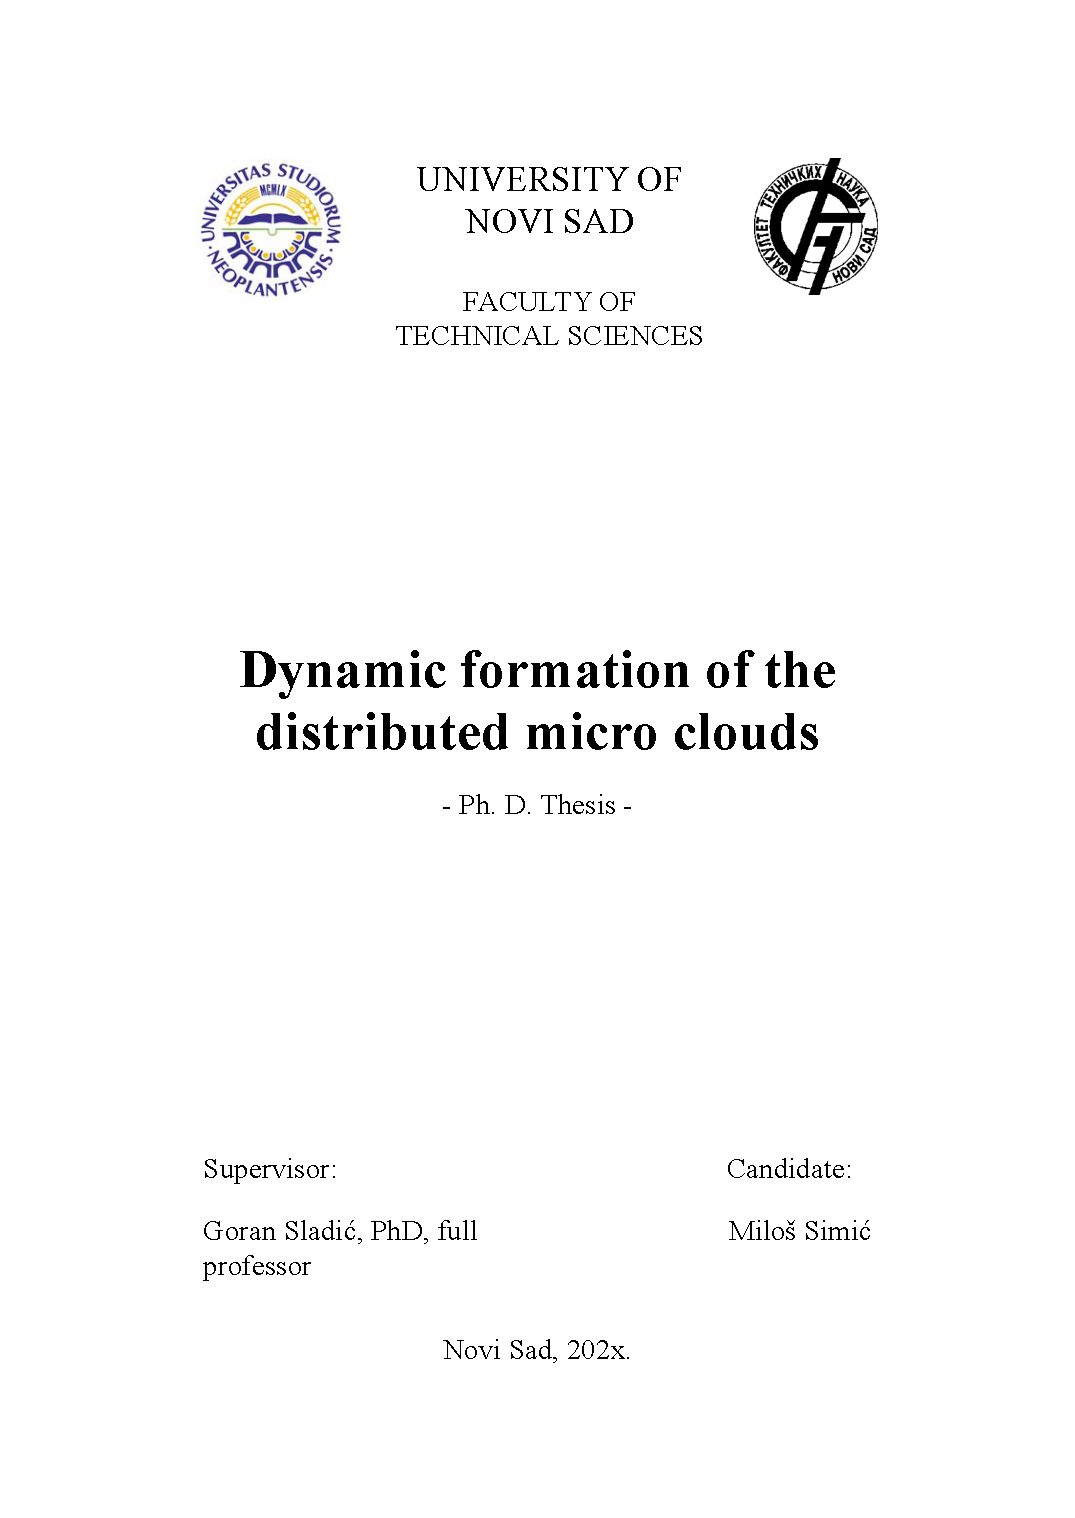
\includepdf[pages=-]{docs/naslovna.pdf}\cleardoublepage 
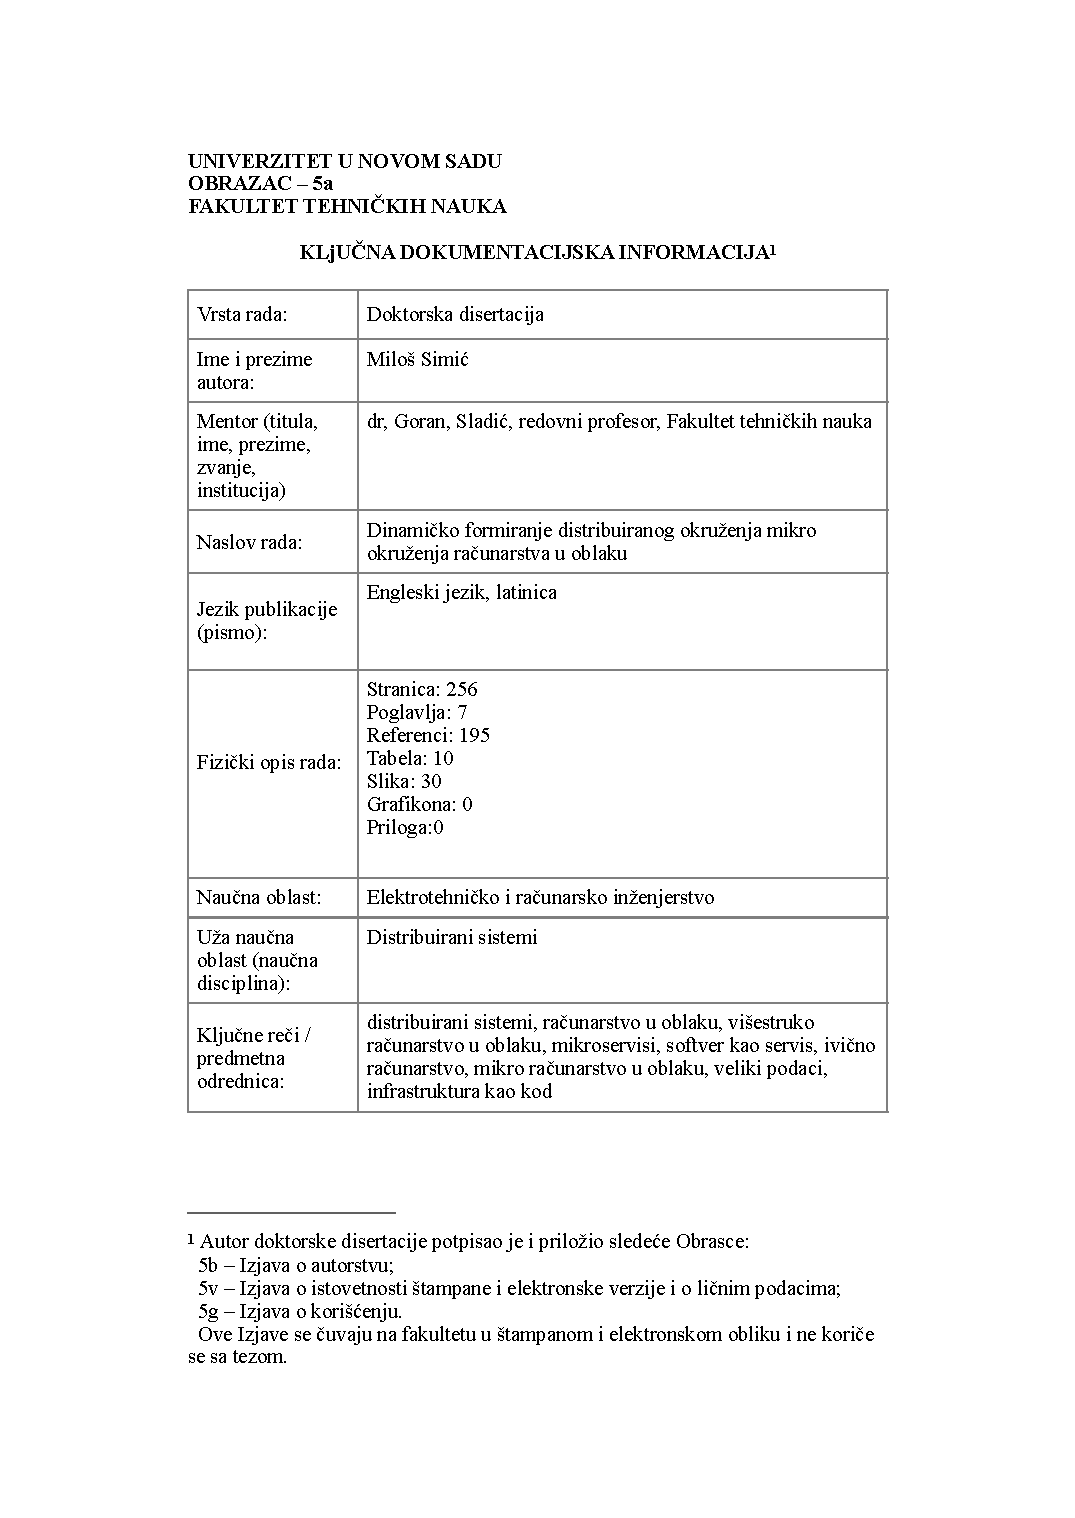
\includepdf[pages=-]{docs/kljucna.pdf}
\pagestyle{empty}
%!TEX root =  main.tex
\chapter*{Acknowledgements}
\pagenumbering{gobble}
%\pagestyle{empty}\cleardoublepage 
%
%
\pagestyle{plain}
\pagenumbering{roman} \setcounter{page}{1}
%
%
\phantomsection
\addcontentsline{toc}{chapter}{Abstract}
%!TEX root =  main.tex
\chapter*{Abstract}
%\pagestyle{empty}
Edge computing brings cloud services closer to the edge of the network, where data originates and dramatically reduces network latency of cloud. It is a bridge linking clouds and the users making the foundation for novel interconnected applications.

However, edge computing still faces many challenges like remote configuration, well defined native applications model, and limited node capacity. It lacks geo-organization and clear separation of concerns. As such edge computing is hard to be offered as a service, for future real-time user-centric applications. 

This thesis presents the dynamic organization of geo-distributed edge nodes into micro data-centers and forming micro-clouds to cover any arbitrary area and expand capacity, availability, and reliability. We use a cloud organization as an influence with adaptations for a different environment, and we present a model for edge applications utilizing these adaptations. 

We argue that the presented model can be integrated into existing solutions or used as a base for the development of future systems. Furthermore, we give a clear separation of concerns for the proposed model. With the separation of concerns setup, edge-native applications model, and a unified node organization, we are moving towards the idea of edge computing as a service, like any other utility in cloud computing. 

The first chapter give introduction to area of distributed systems, narrowing it down to only parts that are important for further understanding of the other chapters and the rest of the thesis in general.

The second chapter, show related work from different areas that are connected or that influenced this thesis. This chapter as well show what is the current state of the art in industry and academia, but also describe positoin of this thesis compred to the related reserach.

The third chapter, propose model that is influenced with cloud computing architectural organizations, but adopted for different environemtn. We presetn how we can separate geographic area into micro data-centers that are zonaly organzied to serve local population and, and forme them dinamicaly. This chapter also give formal models for all protocols used for creation of such a system with separation of concerns, applications models and present limitations of this thesis.

The forth chapter present implemented framweork that is based on model described in chapter three. We describe architecture and in detail every operation framework is able to do with limitations of the framework.

The fith and the last chapter conclud this thesis, and present future work that should be done.\\\\ 

\noindent
\textbf{Key words:} distributed systems, cloud computing, micro clouds, edge computing, platform, as a service model.\cleardoublepage
%
%
\phantomsection
\addcontentsline{toc}{chapter}{Rezime}
%!TEX root =  main.tex
\chapter*{Rezime}
\pagestyle{plain}

Razvojem i razli\v citom primenom softverskih i hardverskih sistema menja se i na\v cin na koji ljudi komuniciraju, u\v ce i realizuju svoje aktivnosti. Kao posledica sve ve\'ce primene ovih sistema u razli\v citim oblastima obim obrade i koli\v cina podataka znatno su se pove\'cali~\cite{ChiangZ16}. Ovo pove\'canje za posledicu je imalo sve ve\'cu upotrebu distribuiranih sistema da bi se ti poslovi mogli obaviti uspe\v sno.

Pro\v sirena stvarnost (AR), igre preko mre\v ze, automatsko prepoznavanje lica, autonomna vozila ili internet stvari (IoT) proizvode izuzetno velike koli\v cine podataka \v sto zna\v cajno uti\v ce na opterećenje kao i na ka\v snjenje~\cite{ChiangZ16}. Ovakvi zahtevi su izvan onoga \v sto se centralizovanim ra\v cunarskim modelima, poput ra\v cunarstva u oblaku, mo\v ze ponuditi~\cite{ChiangZ16}. \v Cak i mali problemi mogu dovesti do velikog zastoja u komunikaciji aplikacija i uslugama od kojih ljudi zavise.  

Primer koji se nedavno desio jo\v s jedan je u nizu otkaza na Amazon Web Services (AWS) platformi~\cite{GunawiHSLSAE16}. Ovim je platforma bila nedostupna korisnicima i aplikacijama, a kao rezultat nedostupnosti platforme velika koli\v cina aplikacija i servisa, koji se izvr\v savaju preko interneta, postaje potpuno nedostupna korisnicima i na kraju neupotrebljiva. 

%Da bi se razumelo kako smo do\v sli do tog problema, prvo se mora razumeti \v sta je zapravo ra\v cunarstvo u oblaku i videti kako se ovaj model organizuje.

Da bi se razumelo kako je problem nastao, potrebno je objasniti \v sta je zapravo ra\v cunarstvo u oblaku, predstaviti organizaciju i definisati arhitekturu ovog ra\v cunarskog modela.

Ra\v cunarstvo u oblaku definisano je kao skup ra\v cunarskih resursa koji se mogu ponuditi korisnicima kroz takozvani uslu\v zni softver~\cite{Vogels}. Hardver i softver u velikim centrima za obradu podataka pru\v zaju usluge svojim korisnicima preko interneta~\cite {AboveTheCloud}. Resursi poput CPU-a, GPU-a, skladi\v sta podataka i mre\v ze mogu se koristiti za nekakvu obradu podataka, ili osloboditi i to na zahtev i po potrebi korisnika~\cite{ZhangCB10}. 

Prednost ra\v cunarstva u oblaku su razni servisi koji su ponu\dj eni korisnicima kao usluge ili uslu\v zni softver~\cite{Vogels}. Tradicionalnim modelom ra\v cunarstva u oblaku pružaju se ogromni procesni i skladi\v sni resursi i to po potrebi, na zahtev korisnika, kako bi se podr\v zale razli\v cite potrebe aplikacija. Ovo svojstvo odnosi se na sposobnost ra\v cunarstva u oblaku da dozvoli korisnicima alokaciju dodatnih resursa ili oslobađanje postoje\'cih, kako bi se podudarali sa radnim optere\'cenjima aplikacija~\cite{AssuncaoVB18}. 

Jedna od problema u ovakvim sistemima nastaje kada je potrebno da se (veliki) podaci prebace sa svog izvori\v sta u oblak. Ovim dolazi do velike latencije ili ka\v snjenja u sistemu~\cite {HossainRH18}. Na primer, Boeing 787 generi\v se pola terabajta podataka po jednom letu, dok autonomni automobil generi\v se dva petabajta podataka tokom samo jedne vo\v znje~\cite{CaoZS18}. 

Me\dj utim, propusni opseg nije dovoljno veliki da bi podr\v zao takve zahteve~\cite{CaoZS18}. Prenos podataka nije jedini problem sa kojim se ra\v cunarstvo u oblaku susre\'ce. Aplikacije kao \v sto su autonomni automobili, bespilotne letelice ili balansiranje optere\'cenja u elektri\v cnim mre\v zama, zahtevaju obradu podataka u realnom vremenu da bi se ispravno donosile odluke i reagovalo na razne promene~\cite{CaoZS18}.

Centralizovana arhitektura ra\v cunarstva u oblaku, sa ogromnim kapacitetima centara za obradu podataka, stvara efikasno upravljanje resursima. Ovom strategijom dolazi se do smanjenja administrativnih tro\v skova celokupnog sistema~\cite{BariBEGPRZZ13}. Me\dj utim, kada takav sistem do\dj e do svojih granica, centralizacija uzrokuje mnoge druge probleme~\cite{GunawiHSLSAE16, LopezMEDHIBFR15}. Uprkos svim prednostima ovog modela, servisi i usluge vremenom se suo\v cavaju sa ozbiljnom degradacijom kvaliteta odziva i performansi usled velike propusnosti i ka\v snjenja~\cite{KarimIWGSYO16}. To mo\v ze dovesti do nesagledivih posledica po poslovanje, ali potencijalno i te\v ze efekte poput uticaja na ljudske \v zivote. 

Razne organizacije koriste usluge ra\v cunarstva u oblaku i oslanjaju se na njega kako bi izbegle izuzetno velike infrastrukturalne investicije~\cite {MonsalveCC18} poput pravljenja i odr\v zavanja sopstvenih centara za obradu podataka. Oni koriste resurse koje su obezbedili drugi pru\v zaoci usluga~\cite{Satyanarayanan17} i pla\'caju shodno tome koliko vremenski koriste usluge --- \emph{a pay as you go} model.

Cilj ove teze je predstavljanje i upotreba formalnih modela na osnovu kojih se mogu opisati, i formalno verifikovati protokoli, kao i implementirati radni okvir za distribuirani sistem, koriste\'ci geografski rasprostranjena okru\v zenja nalik ra\v cunarstvu u oblaku. Opisani sistem mogu koristiti ne samo obi\v cni korisnici, ve\'c ga i pru\v zaoci usluga ra\v cunarstva u oblaku mogu integrisati u svoju platformu i svoje servise kako bi se minimalizovao zastoj kriti\v cnih sistemskih segmenata. \v Citav sistem se mo\v ze posmatrati kao skup distribuiranih mikro oblaka ili sloj obrade podataka, koji u oblak \v salje samo va\v zne podatke, smajuju\'ci tro\v skove korisnicima, ali i obezbe\dj uju\'ci ve\'cu dostupnost usluga ra\v cunarstva u oblaku.

Distribuirani softverski sistemi su prilično slo\v zeni za modelovanje i implementaciju. Jedan od problema u ovakvim sistemima \v cesto nastaje zbog problema u komunikaciji \v cvorova preko mre\v ze koja nije sigurna i pouzdana. Poruke mogu da kasne, mogu da stignu u razli\v citom redosledu ili da ne stignu. Tako\dj e, \v cvorovi u sistemu mogu prestati sa radom potpuno nasumi\v cno stvaraju\'ci dodatne komplikacije. James Gosling i Peter Deutsch, kreirali su listu problema za mre\v zne aplikacije poznate kao \textit{8 zabluda distribuiranih sistema}~\cite{articleRotem}:

\begin{enumerate}[start=1,label={(\bfseries \arabic*)}]
	\item \textbf{Mre\v za je pouzdana.} Uvek \'ce se ne\v sto neplanirano desiti sa mre\v zom koja je prili\v cno nepouzdana - prekid napajanja, prekid kabla, problemi u okru\v zenju, itd.
	\item \textbf{Ka\v snjenje ne postoji.} Lokalno ka\v snjenje nije problem, ali se situacija vrlo brzo pogor\v sava kada se komunikacija oslanja na internet, i slu\v cajeve gde se koristi izuzetno kompleksna mre\v zna komunikacija ra\v cunarstva u oblaku.
	\item \textbf{Propusnost je beskona\v cna.} Iako se \v sirina propusnog opsega stalno pove\'cava i sve je bolja i bolja, srazmerno tome raste i koli\v cina podataka koja se prebacuje na obradu ili skladi\v stenje.
	\item \textbf{Mre\v za je sigurna.} Trendovi internet bezbednosti pokazuju izuzetno veliki rast napada, a ovo jo\v s vi\v se postaje problem u ra\v cunarstvu u oblaku javnog tipa.
	\item \textbf{Topologija se ne menja.} Mre\v zna topologija obi\v cno je izvan kontrole korisnika, a topologija mre\v ze stalno se menja usled brojnih razloga - dodati ili uklonjeni novi ure\dj aji, serveri, prekidi u komunikaciji itd.
	\item \textbf{Postoji samo jedan administrator.} Danas postoje brojni administrativi za veb servere, baze podataka, ke\v s memoriju i sli\v cno, ali, tako\dj e, kompanije sara\dj uju sa drugim kompanijama ili pru\v zaocima usluga ra\v cunarstva u oblaku.
	\item \textbf{Tro\v skovi transporta ne postoje.} Ova tvrdnja nikako nije ta\v cna iz prostog razloga \v sto moramo serijalizovati informacije i podatke koje \v saljemo \v sto dodatno tro\v si resurse i pove\'cava ukupno ka\v snjenje. Ovde nije problem samo u ka\v snjenju, ve\'c u tome \v sto svaka serijalizacija informacija zahteva dodatno vreme i dodatne resurse.
	\item \textbf{Mre\v za je homogena.} Danas je homogena mre\v za izuzetak, a ne pravilo. Postoje razli\v citi serveri, sistemi, klijenti koji komuniciraju. Implikacija ovoga je da, pre ili kasnije, mora se pretpostaviti da je potrebna interoperabilnost izme\dj u ovih sistema. Mogu se koristiti i za\v sti\'ceni protokol koji nisu javno dostupni, koji mogu dodatno tro\v siti vreme. Ovi protokoli mogu ostati bez podr\v ske, pa ih treba izbegavati.
\end{enumerate}

Iako razvoj distribuiranih sistema traje ve\'c nekoliko decenija, problemi koji se javljaju prilikom njihovog razvoja su i dalje identi\v cni. 

Prilikom razvoja distribuiranih sistema, programeri i dizajneri \v cesto zaboravljaju na definisane probleme, \v sto neretko dovodi do izuzetno velikih pote\v sko\'ca. Na\v cin da se to u ranim fazama otkrije jeste kori\v s\'cenje formalnih matemati\v ckih metoda za opisivanje i modelovanje ovih sistema. Ove metode sa\v cinjavaju razne tehnike koje slu\v ze za specifikaciju i verifikaciju kompleksnih sistema i koje su zasnovane na matemati\v ckim i logi\v ckim principima.

Kao odgovor na probleme koji mogu nastati kao posledica ka\v snjenja, nedostupnosti usluga u ra\v cunarstva u oblaku, malicioznih napada, ali i usled kvara nekog od resursa na mre\v zi~\cite{GunawiHSLSAE16}, nastala je nova paradigma tzv. ivi\v cno ra\v cunarstvo (eng. edge computing - EC)~\cite{Satyanarayanan17}. 

EC je model u kome se procesne i skladi\v sne mogu\'cnosti ra\v cunarstva u oblaku prebacuju u blizini izvora podataka~\cite{Satyanarayanan17}. Kao posledicu toga, ra\v cunarstvo u oblaku pro\v sireno je novim mogu\'cnostima. Smanjuje se ka\v snjenje \v sto onda dovodi do novih mogu\'cnosti za aplikacije budu\'ce generacije~\cite{NingLSY20}.   

Tokom prethodnih godina, pojavili su se razni modeli koji spu\v staju obradu i skladi\v stenje podataka bli\v ze izvori\v stu, poput fog ra\v cunarstva~\cite{BonomiMNZ14}, cloudlet-a~\cite {MonsalveCC18} i mobilnih ivi\v cnih ra\v cunara (MEC)~\cite{WangZZWYW17}. U ovoj disertaciji, svi pomenuti modeli se smatraju ivi\v cnim ra\v cunarstvom, a njihovi cvorovi ivi\v cnim \v cvorovima. 

Svi pomenuti modeli koriste koncept prenosa skladi\v snih i procesnih mogu\v cnosti iz oblaka bli\v ze izvorima podataka,~\cite{KhuneP19} dok su zahtevnije obrade i dalje zadr\v zane u oblaku iz vrlo prostog razloga --- dostupnost znatno ve\'ce koli\v cine resursa~\cite{NingLSY20}. EC modeli uvode male servere koji se arhitekturalno nalaze izme\dj u izvora podataka i oblaka. Tipi\v cno je za ove servere da imaju manje mogu\'cnosti u pore\dj enju sa serverima u oblaku~\cite{ChenHLLW15}. 

Prednost malih servera je u tome \v sto se oni mogu nalaziti na razli\v citim lokacijama, na primer u baznim stanicama~\cite{WangZZWYW17}, gradskim centralama, restoranima, bolnicama, \v skolama, kompanijama, ili mogu biti rasprostranjeni po geografskim regionima, a sve to kako bi se izbeglo ka\v snjenje i pove\'cala propusnost~\cite{MonsalveCC18}.   

Oni mogu poslu\v ziti kao za\v stitni sloj~\cite{SatyanarayananK19} ili kao nivo obrade pre nego \v sto podaci budu poslati u oblak. Sa druge strane, korisnici dobijaju jedinstvenu mogu\'cnost dinami\v cke i selektivne kontrole informacija koje bivaju poslate u oblak. 

Jo\v s jednu prednost ovih servera predstavili su Aroca i saradnici~\cite{ArocaG12}. Naime, njihovi rezultati su pokazali da mali serveri zadr\v zavaju dobre performanse prilikom pokretanja zahtevnih aplikacija i klasterskog okru\v zenja. Malo slabije performanse pokazali su u slu\v caju trenutno dostupnih skladi\v sta podataka, ali to mo\v ze biti podsticaj da se polje istra\v zivanja skladi\v sta podataka dopuni novim modelima, optimizovanim za male servere.

Jedan model te\v sko \'ce odgovarati potrebama svih aplikacija u budu\'cnosti, tako da ra\v cunarstvo u oblaku ne bi trebalo da bude na\v sa kona\v cna granica i jedina opcija. Razni modeli, nastali na bazi malih servera, pokazuju mogu\'cnost da se obrada podataka mo\v ze obaviti bli\v ze izvori\v stu, dok te\v ski prora\v cuni mogu ostati u oblaku zbog ve\'ce dostupnosti resursa. U oblak treba slati samo informacije koje su klju\v cne za druge usluge ili aplikacije~\cite{inproceedingsSimic1}, a ne sve kako predla\v ze standardni model oblaka. 

Ideja malih servera sa razli\v citim ra\v cunskim, skladi\v snim i mre\v znim resursima pokre\'ce zanimljive istra\v ziva\v cke ideje i, kao takva, motivacija je za ovu tezu. Kori\v s\'cenje resursa, koji su organizovani lokalno kao mikro oblaci, oblaci zajednice ili ivi\v cni oblaci,~\cite{RydenOCW14} predla\v zu Riden i saradnici.

Usled problema koji mogu nastati u doglednoj budu\'cnosti kori\v s\'cenjem sve ve\'ceg broja ra\v cunarskih sistema koji su povezani na internet, kao i  zbog ograni\v cenja ra\v cunarstva u oblaku u trenutnoj izvedbi, akademska zajednica kao i industrija po\v cele su da istra\v zuju i razvijaju odr\v ziva re\v senja. Neka istra\v zivanja vi\v se su usredsre\dj ena na prilago\dj avanje postoje\'cih re\v senja zahtevima EC-a, dok druga eksperimenti\v su sa novim idejama i re\v senjima.

U svom radu~\cite{GreenbergHMP09} Greenberg i saradnici isti\v cu da se mikro centri za obradu podataka ($\upmu$DCs) koriste prvenstveno kao \v cvorovi u mre\v zama za distribuciju sadr\v zaja i u drugim \say{lo\v se distribuiranim} aplikacijama. $\upmu$DC su zanimljiv model u podru\v cju brzih inovacija i razvoja. Autori uvode koncept $\upmu$DC-a kao centra za obradu podataka koji se nalazi u blizini velike populacije, smanjuju\'ci pritom fiksne tro\v skove tradicionalnih centara za obradu podataka. Samim tim, minimalna veli\v cina $\upmu$DC-a definisana je potrebama lokalnih korisnika~\cite{GreenbergHMP09, AbbasZTS18}, pru\v zaju\'ci agilnost kao klju\v cnu karakteristiku. Ovde agilnost podrazumeva sposobnost dinami\v ckog rasta i smanjenja potrebe za resursima kao i upotrebe resursa sa optimalne lokacije~\cite{GreenbergHMP09}. 

Satyanarayanan i saradnici u svom radu~\cite{SatyanarayananK19} pokazuju da $\upmu$DC-ovi mogu poslu\v ziti kao za\v stitni sloj. Simi\'c i saradnici u svom radu~\cite{inproceedingsSimic1}  opisuju takav sistem kao nivo obrade podataka na njihovom izvoru, dok korisnici dobijaju jedinstvenu mogu\'cnost dinami\v ckog i selektivnog upravljanja informacijama koje se \v salju u oblak. 

Zonska organizacija malih servera, koju su predstavili Guo i saradnici~\cite{GuoRG20} u primeni kod pametnih vozila daje zanimljivu perspektivu o EC-u. Autori su pokazali kako modeli koji dele oblast na zone omogu\'cavaju kontinuitet dinami\v ckih usluga i smanjuju primopredaju veze. Tako\dj e, pokazali su kako da se pokrivenost malim serverima prenese na ve\'cu zonu, \v cime se pro\v siruju ra\v cunarska snaga i kapacitet skladi\v stenja podataka.

EC poti\v ce iz peer-to-peer sistema, kako su to pretpostavili Lopez i saradnici, ali ga pro\v siruju u novim pravcima i pru\v zaju mogu\'cnost integracije sa ra\v cunarstvom u oblaku~\cite{LopezMEDHIBFR15}.

U svom radu, Kurniawan i saradnici~\cite{inbookKurniawan} pokazali su vrlo lo\v su skalabilnost u centralizovanim modelima mre\v za za isporuku sadr\v zaja(CDN) u oblaku. Autori su predlo\v zili decentralizovano re\v senje koriste\'ci nano centre za obradu podataka koje \v cine mre\v zni ure\dj aji u ku\'ci~\cite{inbookKurniawan}. Ovi centri za obradu podataka opremljeni su, tako\dj e, sa ne\v sto skladi\v snog prostora. Pokazana je mogu\'ca upotreba nano centara za obradu podataka \v cak i za neke velike primene sa jednom izuzetno bitnom predno\v s\'cu - mnogo manjom potro\v snjom energije.

$\upmu$DC-ovi sa zonskom organizacijom servera dobra su polazna osnova za izgradnju EC-a (koja mo\v ze biti ponu\dj ena kao servis korisnicima), ali i mikro ra\v cunarstva u oblaku jer se mo\v ze relativno jednostavno pro\v siriti ra\v cunarska snaga i skladi\v sni kapacitet koji opslu\v zuju lokalne korisnike. Me\dj utim, da bi se to postiglo, potreban nam je dostupniji i elasti\v cniji sistem sa manje ka\v snjenja. 

Dizajn ra\v cunarstva u oblaku je takav da svaki deo doprinosi otpornijem i skalabilnom sistemu. Regioni ili centri za obradu podataka izolovani su i nezavisni jedni od drugih, a takođe sadr\v ze resurse koji su potrebni aplikacijama za nesmetan rad. Regioni su sa\v cinjeni od nekoliko dostupnih zona~\cite{SouzaMFAK19} i ako neka od zona postane nedostupna, druge zone preuzimaju opslu\v zivanje korisni\v ckih zahteve i time ceo sistem, kao celina, nastavlja neometan rad. Po uzoru na ovakvu arhitekturu, EC bi mogli koristiti vrlo sli\v cnu strategiju formiraju\'ci model mikro ra\v cunarstva u oblaku ($\upmu$C), gde se mali serveri ili \v cvorovi grupi\v su u \emph{klastere}, a vi\v se klastera u ve'cu logi\v cku celinu nazvanu \emph{region}, pove\'cavaju\'ci dostupnost i pouzdanost sistema i njegovih aplikacija.

U tom kontekstu, pod $\upmu$C-om smatraju se geografski rasprostranjeni distribuirani sistemi koji organizaciono li\v ce na ra\v cunarstvo u oblaku, ali se nalaze u neposrednoj blizini korisnika i opslu\v zuju njihove zahteve. Ta razlika pru\v za druga\v ciju organizaciju nego u standardnom modelu ra\v cunarstva u oblaku. 

Koncept regiona u ra\v cunarstvu oblaka je fizi\v cki element~\cite{SouzaMFAK19}, dok se u $\upmu$C-u pojam \emph{region} mo\v ze koristiti za opisivanje skupova \emph{klastera} \v cvorova preko proizvoljne geografske oblasti. Regioni se sastoje od najmanje jednog klastera, ali mogu se sastojati i od vi\v se njih tako da se postigne otporniji, skalabilniji i dostupniji sistem. 

Da bi se osiguralo manje ka\v snjenje u sistemu, u normalnim okolnostima treba izbegavati veliku udaljenost izme\dj u klastera. U tradicionalnom modelu ra\v cunarstva u oblaku pro\v sirenje regiona zahteva fizi\v cko povezivanje novih modula sa ostatkom infrastrukture~\cite{Hamilton07}, \v sto mo\v ze izazvati nedostupnost tog regiona neko vreme.
 
U $\upmu$C-u regioni mogu prihvatiti nove ili osloboditi postoje\'ce klastere. Isto tako i klasteri mogu prihvatiti nove ili osloboditi postoje\'ce \v cvorove \emph{dinami\v cki} bez direktnog povezivanja novih modula. Vi\v se regiona \v cine novi logički sloj --– \emph{topologiju}. 

Topologija se sastoji od najmanje jednog regiona, a mo\v ze se prostirati i na vi\v se regiona. Prilikom dizajniranja topologije, posebno ako regioni treba da dele informacije ili da na neki na\v cin sara\dj uju, po\v zeljno je izbegavati veliku udaljenost izme\dj u regiona ako je to mogu\'ce, da bi se smanjilo ka\v snjenje u sistemu. 

Primenom  \emph{klastera}, \emph{regiona} i \emph{topologije} mogu\'ce je pokriti bilo koju geografsku oblast sa sposobno\v s\'cu da se smanje ili pro\v sire postoje\'ci \emph{klasteri}, \emph{regioni} pa \v cak i \emph{topologije}.  

Organizacija \emph{klastera, regiona i topologija} u $\upmu$C-u isklju\v civo je stvar potrebe korisnika, i kao takva sli\v cna je modeliranju u sistemima velikih podataka ~\cite{SonbolOAA20, WangCAL14}. Na primer, klasteri mogu obuhvatiti \v citav jedan grad ili manji koji obuhvataju ure\dj aji u jednom doma\'cinstvu i sve izme\dj u ova dva ekstrema. Grad bi mogao predstavljati jedan region, sa delovima grada koji su organizovani u klastere. Topologija grada mo\v ze se formirati tako \v sto se grad podeli na vi\v se regiona koji sadr\v ze vi\v se klastera. Topologija dr\v zave mo\v ze se formirati tako \v sto se kroz prirodne i/ili administrativne regije defini\v su regioni, iako je i bilo koja druga podela mogu\'ca.

\v Cvorovi unutar svakog klastera treba da izvr\v savaju neki od protokola za odr\v zavanje definicije klastera odnosno pripadnosti \v cvorova klasteru. Neki od \textit{Gossip} protokola poput \textit{SWIM}-a~\cite{DasGM02} mogu se koristiti u saradnji sa mehanizmima replikacije podataka~\cite {LiBCL20, CauCBFCEB16, CRDTS_Nuno} \v cine\'ci ceo sistem otpornijim na potencijalne gre\v ske. Treba prihvatiti \v cinjenicu da \'ce \v cvorovi u takvom sistemu iz raznih razloga biti nedostupni. To se ne mo\v ze izbe\'ci, ali se sistem mo\v ze projektovati tako da servisi ipak budu ipak budu dostupni koriste\'ci pritom neki od kopija servisa.

U modelu koji opisuje razne resurse kao usluge~\cite{DuanFZSNH15} EC i mikro ra\v cunarstvo u oblaku nalaze se izme\dj u CaaS-a i PaaS-a, u zavisnosti od potreba korisnika.

Prethodno definisan model $\upmu$C mogao bi se ponuditi kao usluga korisnicima kao i bilo koji drugi resurs ra\v cunarstva u oblaku. U slu\v caju kada je potrebno vi\v se resursa na jednoj strani, mogu\'ce ih je reorganizovati da se iskoriste gde su oni stvarno potrebni. Sa druge strane, kompanije koje pru\v zaju usluge ra\v cunarstva u oblaku mogu integrisati predlo\v zeni model u svoj postoje\'ci sistem, skrivaju\'ci nepotrebnu slo\v zenost iza nekog komunikacionog interfejsa ili predlo\v zenog modela aplikacije ili usluge.

Da bi se i EC modeli mogli iskoristiti na ovaj na\v cin potrebna je jasna dinami\v cka organizacija geografski raspore\dj enih \v cvorova, dobro definisan model aplikacija i jasno razdvajanje nadle\v znosti u sistemu. Kao takvi, bili bi jako slo\v zeni da se ponude kao usluga korisnicima. 

EC sistemi obi\v cno postoje nezavisno jedni od drugih, rasuti bez me\dj usobne povezanosti i saradnje. Nude ih pru\v zaoci usluga koji korisnike uglavnom ograni\v cavaju na usluge unutar sopstvenog ekosistema, \v cesto bez mogu\'cnosti izbora servisa van njihovog kataloga usluga. 

Grupisani čvorovi treba da budu organizovani lokalno, \v cine\'ci sistem kompletnim, a aplikacije dostupnijim i pouzdanijim, pro\v siruju\'ci resurse izvan pojedina\v cnog \v cvora ili male grupe \v cvorova. Takav sistem treba da odr\v zava dobre performanse za izgradnju servera i klastera~\cite{ArocaG12}.

Da bi se postiglo takvo pona\v sanje, neophodno je imati dinami\v cko upravljanje resursima i upravljanje ure\dj ajima. Potrebno je uvek imati dostupne informacije o resursima, konfiguraciji i zauzetosti \v cvorova~\cite{GubbiBMP13, WangZZWYW17} i klastera u celini. Tradicionalni centri za obradu podataka predstavljaju dobro organizovan i povezan sistem. Sa druge strane, $\upmu$DC-ovi se sastoje od razli\v citih ure\dj aja koji to nisu~\cite{JiangCGZW19}. Ovaj problem dovodi nas do problema kojim se bavi ova teza.

Da bi opisali fizi\v cke usluge, Jin~\cite {JinCJL14} i saradnici predla\v zu tri osnovna koncepta i preciziraju njihove odnose. Ovi koncepti su: \textbf{(1)} ure\dj aji, \textbf{(2)} resursi i \textbf{(3)} servisi. 

Podela nadle\v znosti bitan je deo svakog sistema, posebno ako se stvara platforma koja se nudi korisnicima kao usluga. Model podele nadle\v znosti, koji ova teza predla\v ze, zasnovan je na ovim konceptima, prilago\dj en druga\v cijem slu\v caju kori\v s\'cenja i  podeljen u tri sloja \v: \textbf{(1)} ure\dj aje, \textbf{(2)} resurse, i \textbf{(3)} servise.

Prvi sloj \v cine razli\v citi ure\dj aji odnosno kreatori podataka i korisnici usluga odnosno servisa. Drugi sloj predstavlja resurse, koji imaju prostorne karakteristike i ukazuju na mogu\'cnosti za obradu odnosno skladi\v stenje podataka \v cvorova na kojima se izvr\v savaju~\cite{JinCJL14}. Programeri u bilo kom trenutku moraju znati iskori\v s\'cenost resursa kao i stanje i dostupnost aplikacija. 

Resursi predstavljaju EC \v cvorove i, da bi \v cvor bio deo sistema, mora zadovoljiti \v cetiri jednostavna pravila: 

\begin{enumerate}[start=1,label={(\bfseries \arabic*)}]
\item Mora biti sposoban da pokrene operativni sistem sa sistemom datoteka;
\item Mora biti u mogu\'cnosti da pokrene neki od dostupnih alata za izolaciju aplikacija, na primer \textit{container} ili \textit{unikernel}; 
\item Mora imati dostupne resurse za kori\v s\'cenje (npr. CPU, GPU, disk itd.);
\item Mora imati internet vezu.
\end{enumerate}

Tre\'ci sloj cine servisi koji pruzaju resurse aplikacijama putem definisanog interfejsa i \v cine ih dostupnim preko interneta~\cite {JinCJL14}. Oni odmah odgovaraju na klijentske zahteve, ako je to mogu\'ce, ili mogu da skladi\v ste prona\dj enu informaciju za neke budu\'ce korisni\v cke upite~\cite {SatyanarayananBCD09, YaoXWYZP20}. Servisi koji se izvr\v savaju u oblaku treba da budu u stanju da prihvate unapred obra\dj ene podatke i odgovorni su za obradu i skladi\v stenje podataka \v ciji kapacitet prevazilazi mogu\'cnosti EC \v cvorova. Ovi servisi tako\dj e treba da budu zamenska opcija u slu\v caju da prethodno definisani sistem bude nedostupan iz bilo kog razloga.

Razdvajanjem nadle\v znosti modela i objedinjenjem organizacije \v cvorova, te\v zi se ka pristupu EC-a kao usluge i mogu\'cnosti dinami\v ckog formiranja distribuirnaih mikro oblaka koji bi mogli da obrade podatke na samom njihovom izvoru.

Me\dj utim, infrastruktura za takav sistem ne\'ce biti potpuno efikasna sve dok proces konfigurisanja i kori\v s\'cenja ne bude zna\v cajno pojednostavljen~\cite{SatyanarayananBCD09}. Ru\v cno pode\v savanje \v cvorova predstavlja naporan i dugotrajan proces, naro\v cito kada se uzme u obzir geografska rasprostranjenost dostupnih \v cvorova. 

Model koji se predla\v ze u ovoj tezi re\v sava gorepomenuti problem pomo\'cu  dinami\v ckog pode\v savanja i formiranja klastera, regiona i topologija i oslanja se na \v cetiri protokola:

\begin{enumerate}[start=1,label={(\bfseries \arabic*)}]
	\item \textbf{Provera stanja \v cvora} - protokol obave\v stava sistem o stanju svakog \v cvora; 
	\item \textbf{Formiranje klastera} - protokol formira nove klastere, regione i topologije;
	\item \textbf{Provera idempotencije} - protokol proverava da li klaster, region ili topologija postoje, i da li je potrebno pokrenuti protokol za formiranje;
	\item \textbf{Pregled detalja} - protokol prikazuje trenutno stanje sistema korisniku kroz razne nivoe detalja.
\end{enumerate}

Za formalni opis server ili \v cvorovi (u disertaciji ovi pojmovi se koriste naizmeni\v cno) u sistemu, kori\v s\'cena je teorija skupova. Prethodno definisane protokole mogu\'ce je formalno modelirati upotrebom~\cite{HuY17} pro\v sirenje \emph{multiparty asynchronous session types} (MPST)~\cite {HondaYC08} - klasa tipova pona\v sanja formirana za opisivanje distribuiranih protokola oslanjaju\'ci se na asinhrone komunikacije.

Ova matemati\v cka terorija se mo\v ze iskoristitit i za verifikaciju, da li definisani protokoli zadovoljavaju MPST sigurnost (nema dostupnog stanja gre\v ske) i napredak (akcija se na kraju izvr\v sava, pod pretpostavkom po\v stenja).

Proces modelovanja odvija se u dva koraka:

\begin{enumerate}[start=1,label={(\bfseries \arabic*)}]
	\item \textbf{Prvi korak} u modeliranju komunikacija sistema pomo\'cu MPST teorije predstavlj definisanje \emph{globalnog tipa}, \v sto predstavlja globalni opis celokupnog protokola sa neutralne ta\v cke posmatranja.
	\item \textbf{Drugi korak} u modeliranju komunikacija sistema pomo\'cu MPST teorije je pru\v zanje sintaksi\v cke projekcije protokola na svakog u\v cesnika u komunikaciji iskazane kao \emph{lokalni tip}, koji se zatim koristi za proveru tipa i implementacije krajnje ta\v cke.
\end{enumerate}

Na osnovu prethodno opisanih ideja i mogu\'cnosti, defini\v se se problem koji ova teza obra\dj uje kroz slede\'ca tri istra\v ziva\v cka pitanja:

\begin{enumerate}[start=1,label={(\bfseries \arabic*)}]\label{rez:questions}
	\item Kako se mo\v ze definisati formalan pro\v siriv model sa jasnom podelom nadle\v znosti, po ugledu na organizaciju ra\v cunarstva u oblaku, koji bi bio prilago\dj en druga\v cijem okru\v zenju izvr\v savanja sa jasnim aplikativnim modelom koji \'ce moći da iskoristi novu, prilago\dj enu arhitekturu?
	\item Kako je mogu\'ce ovako organizovane \v cvorove predstaviti kao uslugu korisnicima za razvoj budu\'cih aplikacija, po poznatom modelu naplate po utro\v sku (eng. pay as you go)?
	\item Kako se mo\v ze definisati formalno ispravan model koji \'ce biti lak za pro\v sirenje?
\end{enumerate}

Ako su prethodna istra\v ziva\v cka pitanja potvrdna, onda pro\v sirenje nalik na oblak pro\v siruje resurse van granica pojedina\v cnog \v cvora \v sto \v citav sistem, kao i same aplikacije koje bi se izvr\v savale u njemu, \v cini dostupnijim i pouzdanijim.

Na osnovu prethodno definisanih istra\v ziva\v ckih pitanja i motivacija, definisane su sledece hipoteze:

\begin{enumerate}[start=1,label={(\bfseries \arabic*)}]
	\item \textbf{Hipoteza:} \textit{Mogu\'ce je organizovati \v cvorove na standardni na\v cin, zasnovan na arhitekturi ra\v cunarstva u oblaku i prilago\dj en druga\v cije rasprostranjenom geografskom okru\v zenju pru\v zaju\'ci korisnicima mogu\'cnost da na najbolji mogu\'ci na\v cin organizuju \v cvorove i klastere po raznim geografskim oblastima kako bi opslu\v zivali samo lokalne korisnike u neposrednoj blizini --- model distribuiranog mikro okru\v zenja ra\v cunarstva u oblaku.}
	\item \textbf{Hipoteza:} \textit{Model distribuiranog mikro okru\v zenja ra\v cunarstva u oblaku se mo\v ze iskoristiti za upravljanje infrastrukturnim resursima u blizini korisnika. Ako je potrebno vi\v se resursa na jednoj strani, mo\v ze se uzeti odre\dj ena koli\v cina resursa i reorganizovati u skladu sa potrebama sistema, ili se mogu reorganizovati na bilo koji drugi \v zeljeni na\v cin.}
	\item \textbf{Hipoteza:} \textit{Mogu\'ce je predstaviti jasnu podelu nadle\v znosti za budu\'ci sistem, koji bi se pru\v zio korisnicima kao usluga, i uspostaviti dobro organizovan sistem u kojem svaki deo ima intuitivnu i jasnu ulogu.}
	\item \textbf{Hipoteza:} \textit{Mogu\'ce je predstaviti objedinjeni model, koji podr\v zava heterogene \v cvorove, sa jasnim setom tehni\v ckih zahteva koje budu\'ci \v cvorovi moraju ispuniti ako \v zele da postanu deo sistema.}
	\item \textbf{Hipoteza:} \textit{Mogu\'ce je predstaviti jasan aplikativni model, intuitivan korisnicima, kako bi se mogao iskoristiti puni potencijal predstavljenog re\v senja.}
\end{enumerate}

Iz prethodno definisanih hipoteza izvode se primarni ciljevi ove teze pri \v cemu o\v cekivani rezultati uklju\v cuju slede\'ce:

\begin{enumerate}[start=1,label={(\bfseries \arabic*)}]
	\item \textit{Definisanje formalnog pro\v sirivog modela sa jasnom podelom nadle\v znosti, po ugledu na organizaciju ra\v cunarstva u oblaku, koji bi bio prilago\dj en okru\v zenju gde se obrada i skladi\v stenje vrše bli\v ze korisnicima sa jasnim aplikativnim modelom koji \'ce mo\'ci da iskoristi novu prilago\dj enu arhitekturu. Ovaj cilj odnosi se na prvo istra\v ziva\v cko pitanje, a definisano je kroz poglavlje \ref{chapter:Micro_clouds}.}
	\item \textit{Definisani model je dostupniji i elasti\v can sa manje ka\v snjenja u pore\dj enju sa pojedina\v cnim malim serverima i mo\v ze se koristiti kao bilo koja druga usluga u oblaku. Ovaj cilj odnosi se na prvo istra\v ziva\v cko pitanje, a definisano je kroz poglavlja \ref{chapter:Micro_clouds} i \ref{chapter:Model usability}.}
	\item \textit{Implementacija i verifikacija prototipa kojim bi se potvrdila prakti\v cna primenljivost navedenog modela i identifikovale sve njegove prednosti i eventualni nedostaci. Ovo se odnosi na tre\'ce istra\v ziva\v cko pitanje i tema je poglavlja \ref{chapter:Micro_clouds} i \ref{chapter:Implementation}.}
\end{enumerate}

\noindent
Ovim istra\v zivanjem predstavlja se jedno mogu\'ce re\v senje za organizaciju geografski rasprostranjenog $\upmu$C-a sa EC \v cvorovima, zasnovano na organizaciji ra\v cunarstva u oblaku, prilago\dj eno obradi i skladi\v stenju podataka u blizini korisnika, a organizovano kroz tri koncepta: \emph{topologiju, region i klaster}. 

Primenom ovih koncepata mogu\'ce je opisivanje bilo kog geografskog podru\v cja u cilju dobijanja dostupnijeg i pouzdanijeg sistema. Organizacija i reorganizacija ovih elemenata vr\v si se dinami\v cki, opisom \v zeljenog stanja sistema, a veli\v cina regiona, klastera i topologija odre\dj uje se prema potrebama klijenata koje se opslu\v zuje.

Ishod istrazivanja je pro\v sirenje nalik na ra\v cunarstvo u oblaku koje pro\v siruje resurse van granica pojedina\v cnog \v cvora \v sto \v citav sistem kao i same aplikacije koje bi se izvr\v savale u okviru njega \v cini dostupnijim i pouzdanijim. Primarna primena jeste u organizaciji geografski distribuiranih ra\v cunarskih resursa na efikasan na\v cin tako da opslu\v zuje korisnike u neposrednoj blizini. 

Prototipsko re\v senje bazirano na prethodnom modelu se razvija kao alat otvorenog koda tako da je njegova primena mogu\'ca u razli\v citim sistemima od strane drugih istra\v ziva\v ckih ili razvojnih timova. Tako\dj e, mo\v ze se koristiti kao samostalno re\v senje tamo gde se kasnije mogu dodati potrebni podsistemi, ali tako\dj e pru\v za mogu\'cnost integracije u postoje\'ca re\v senja.

Predstavljeno re\v senje se mo\v ze koristiti kao pomo\'c ra\v cunarstvu u oblaku prilikom obrade velike kori\v cine podataka, kao sloj koji bi vr\v sio preliminarnu obradu na samom izvori\v stu podataka. Skladi\v stenje i obrada se vr\v si samo za podatke od zna\v caja, \v sto je jako bitno za tipove aplikacija koje bi se izvr\v savale u realnom vremenu zato \v sto sistem lokalno mo\v ze da reaguje znatno br\v ze nego udaljeni sistem ra\v cunarstva u oblaku.

Predstavljeno je preslikavanje ra\v cunarstva u oblaku na EC, i prikazan je formalni model sistema sa jasnom podelom nadle\v znosti i modelom aplikacije za budu\'ci EC koji bi bio ponu\dj en korisnicima kao usluga. Dati su primeri domena gde bi sistem mogao da se koristi zajedno sa primerima aplikacija od kojih bi korisnici imali benefit. 

\noindent
Teza je organizovana u pet poglavlja.

U \textbf{poglavlju~\ref{chapter:Intro}} dat je opis motivacije sa jasno definisanim istra\v ziva\v ckim pitanjima i hipotezama na koje \v zelimo da odgovorimo ovom tezom.

U \textbf{poglavlju~\ref{chapter:Field_overview}} predstavljen je kratak uvod u temu distribuiranih sistema, sa fokusom na podru\v cja koja su va\v zna za razumevanje ove teze i svih njenih delova.

Pokazano je \v sta su distribuirani sistemi ili kako neki sistem mo\v zemo opisati ili posmatrati kao distribuirani sistem. Predstavili smo probleme koje ovi sistemi stvaraju i za\v sto ih je tako te\v sko implementirati, koristiti i odr\v zavati.

Tako\dj e, predstavljeno je nekoliko primera distribuiranih ra\v cunarskih aplikacija koje mo\v zemo primeniti za efikasno iskori\v s\'cavanje velikog broja \v cvorova u distribuiranom sistemu. Dalje, pokazano je \v sta je skalabilnost i za\v sto je ona va\v zna za distribuirane sisteme sa nekoliko primera organizacionih mogu\'cnosti, poput peer-to-peer i master-slave sistema, kao i protokola za opis grupa ili zajednica \v cvorova koji sara\dj uju, a koji su va\v zni u distribuiranom okru\v zenju iz razli\v citih razloga. Dati su primeri raznih varijanti ra\v cunarstva u oblaku koje mo\v zemo iskoristiti za svoje potrebe.

Zatim, pokazano je nekoliko tehnika virtuelizacije koje se mogu koristiti i raspore\dj ivanje kako aplikacija, tako i infrastrukture. Prikazane su razne tehnike bitne za raspore\dj ivanje aplikacija i infrastrukture u okru\v zenju ra\v cunarstva u oblaku, ali i razliku izme\dj u distriburanih sistema i nekoliko modela koji se \v cesto smatraju distribuiranim poput paralelnog i decentralizovanog ra\v cunarstva.

Poglalvje \textbf{poglavlju~\ref{chapter:Review}} daje pregled relevatne literature iz oblasti disertacije.

Prikazali smo razli\v cite platforme, gde autori menjaju ili prilago\dj avaju postoje\'ca re\v senja (kao \v sto su Kubernetes ili OpenStack) da rade u oblastima poput ivi\v cnog ra\v cunarstva i mobilnog ra\v cunarstva. Dalje smo predstavili implementacije nekoliko platformi koje koriste \v cvorove, a koje su korisnici ponudili na dobrovoljnoj bazi, da bi se izvr\v sila nekakva obrada ili skladi\v stenje podataka na njima, kao na primer drop computing i Nebule izme\dj u ostalih.

Pokazali smo kako \v cvorovi mogu biti organizovani po geografskim podru\v cjima na zone, ali i kako mikro centri za obradu podataka mogu da pomognu ra\v cunarstvu u oblaku da prihvata zahteve lokalnih klijenata koji koriste resurse u neposrednoj blizini. Dalje smo opisali razli\v cite tehnike kako se zadaci sa mobilnih ure\dj aja mogu prebaciti na ivi\v cne \v cvorove, ali tako\dj e i razli\v cite modele primene koji bi mogli iskoristiti ove tehnike.

Na kraju ovog poglavlja dato je pore\dj ejne rezultata i doprinosa istrazivanja ove teze u odnosu na slicna istra\v zivanja.

\textbf{Poglavlje~\ref{chapter:Micro_clouds}} \v cini sr\v z ove teze. U ovom poglavlju razdvojili smo sve najva\v znije aspekte koje treba da zadovoljimo kako bi se omogu\'cilo re\v savanja problema kao \v sto su ka\v snjenje i obrada podataka, posebno u doba mobilnih ure\dj aja i IoT-a.

Predlo\v zeni model zasnovan je na $\upmu$DC-ima koji su zonski organizovani i koji \'ce opslu\v zivati lokalne korisnike ili korisnike u blizini. Predstavili smo model koji se zasniva na ra\v cunarstvu u oblaku, ali je prilago\dj en za druga\v ciji scenario i sli\v cne slu\v cajeve kori\v s\'cenja.

Pokazali smo kako mo\v zemo dinami\v cki formirati nove klastere, regione i topologije i kako ih mo\v zemo koristiti zajedno sa mobilnim ure\dj ajima i aplikacijama poput internet stvari (IoT). Ovaj novoformirani sistem oslanja se na jasan model podele nadle\v znosti, usvojen iz postoje\'cih istra\v zivanja i prilago\dj en za novu troslojnu arhitekturu. Formirani model mo\v ze da slu\v zi kao sloj za obradu podataka na samom izvori\v stu ili skoro na samom izvori\v stu, kao sloj za za\v stitu privatnosti korisnika i kontrolu sadr\v zaja koji se \v salje u oblak. Predstavljeni sistem izuzetno je prilagodljiv i podlo\v zan pro\v sirivanju prema razli\v citim dimenzijama, odnosno potrebama i zahtevima.

Predstavljeni model mo\v ze da obhvata ve\'ce ili manje geografske regione. Predstavili smo kako programeri mogu iskoristiti novu infrastrukturu i koji sve modeli aplikacija mogu postojati, ali i kako administratori mogu rasporediti razvijene servise na novoformiranu infrastrukturu koriste\'ci opisni ili deskriptivni model, umesto eksplicitnog slanja komandi i koraka sistemu.

Pred kraj ovog poglavlja, prikazano je kako se isti mo\v ze koristiti kao sastavni deo postoje\'cih sistema (kao skladi\v ste informacija o \v cvorovima) ili se mo\v ze koristiti kao novi model u kom mo\v zemo razviti nove podsisteme. Predstavili smo protokole za stvaranje takvog sistema i modelirali ih koriste\'ci formalne matemati\v cke metode ili, konkretno, teoriju asinhronih tipova sesija.

U \textbf{poglavlju~\ref{chapter:Implementation}} pokazali smo implementirani zasnovan na prethodno predstavljenom modelu. Ovde smo tako\dj e detaljno opisali operacije koje se mogu obaviti u prototipu, ali i kako se implementirani model uklapa i gde mu je mesto u prethodno opisanom modelu podele nadle\v znosti.

Dalje smo izneli rezultate na\v sih eksperimenata u kontrolisanom okru\v zenju kao i ograni\v cenja implementiranog radnog okvira u trenutnoj fazi razvoja. Tako\dj e, opisali smo mogu\'ce primene ovog sistema, ali i to gde bi ovaj model mogao da se koristi kada bi u\v sao u upotrebu.

\textbf{Poglablje}~\ref{chapter:Model usability} prikazuje upotrebljivost predlo\v zenog modela, sa mogu\'cim scenarijima primene. Predstavljen je i jedan konkretan primer kontrole saobra\'caja i usmeravanje ambulantih vozila i medicinskog osoblja do najbli\v ze bolnice u gradu Milanu, Italija, zahva\'cenim COVID-19 virusom, i kako bi predlo\v zeni sistem mogao da se iskoristi da pomogne medicinskom osoblju pri le\v cenju pacijenata, ali i istra\v ziva\v cima u boljem razumevanju samog virusa.

\textbf{Poglavlje~\ref{chapter:Conclusion}} predstavlja poslednje poglavlje ove teze. U ovom poglavlju sumirali smo doprinose ove teze, dali smo ograni\v cenja predlo\v zenog modela i ,ujedno, ove teze, ali i svega onoga \v cega moramo biti svesni \textbf{ako} ako takva tehnologija bude kori\v s\'cena u realnim situacijama. Na samom kraju poglavlja dali smo pregled \v sta se mo\v ze uraditi u pogledu budu\'cih pravaca istra\v zivanja.\\\\

\noindent
\textbf{Klju\v c re\v ci:} distribuirani sistemi, ra\v cunarstvo u oblaku, vi\v sestruko ra\v cunarstvo u oblaku, mikroservisi, softver kao servis, ivi\v cno ra\v cunarstvo, mikro ra\v cunarstvo u oblaku, veliki podaci, infrastruktura kao kod.\cleardoublepage 
 %
 %
\renewcommand{\contentsname}{Table of Contents}
\tableofcontents \cleardoublepage 
\listoffigures \cleardoublepage 
\listoftables \cleardoublepage
\addcontentsline{toc}{chapter}{Listings}
\lstlistoflistings \cleardoublepage

\cleardoublepage 
\listofmyequations
%
%
\cleardoublepage
\phantomsection
\addcontentsline{toc}{chapter}{List of Abbreviations}
\vspace*{1.95cm} \hspace*{-1cm} %,88
\textbf{{\huge List of Abbreviations}\\}
\vspace*{1cm}	
\begin{acronym}[WWWW]
	\acro{API}{Application programming interface}
	\acro{AWS}{Amazon Web Services}
	\acro{CC}{Cloud computing}
	\acro{CDN}{Content delivery networks}
	\acro{CQRS}{Command Query Responsibility Segregation}
	\acro{CRDTs}{Conflict-free replicated datatypes}
	\acro{CSP}{Communicating Sequential Processes}
	\acro{CaaS}{Container as a service}
	\acro{DBaaS}{Databae as a service}
	\acro{DCs}{Data centers}
	\acro{DC}{Distributed computing}
	\acro{DHT}{Distributed Hash Table}
	\acro{DNS}{Domain Name System}
	\acro{DSL}{Domain specific language}
	\acro{DS}{Distributed systems}
	\acro{Dp}{Distributed programmig}
	\acro{ECC}{Edge-centric computing}
	\acro{EC}{Edge computing}
	\acro{ES}{Edge servers}
	\acro{GC}{Garbage collection}
	\acro{IaC}{Infrastructure as code}
	\acro{IaS}{infrastructure as software}
	\acro{IaaS}{Infrastructure as a service}
	\acro{IoT}{Internet of Things}
	\acro{LLTs}{Long-lived transactions}
	\acro{LLT}{long-lived transaction}
	\acro{MANETs}{Mobile Ad-Hoc Networks}
	\acro{MA}{Evolutionary Memetic Algorithm}
	\acro{MCC}{Mobile cloud computing}
	\acro{MEC}{Mobile edge computing}
	\acro{MPST}{Multiparty asynchronous session types}
	\acro{NaCl}{Native Client}
	\acro{NoSQL}{Not Only SQL}
	\acro{OS}{Operating system}
	\acro{P2P}{Peer-to-peer}
	\acro{PaaS}{Platform as a service}
	\acro{QoE}{Quality of experience}
	\acro{QoS}{Quality of service}
	\acro{RAID}{Redundant Array of Inexpensive Disks}
	\acro{REST}{Representational state transfer}
	\acro{RPC}{Remote procedure call}
	\acro{SDN}{Software-defined networks}
	\acro{SEC}{Strong Eventual Consistency}
	\acro{SPOF}{Single Point of Failure}
	\acro{SRE}{Site Reliability Engineering}
	\acro{SaaS}{Software as a service}
	\acro{SoC}{Separation of concerns}
	\acro{TTL}{Time to live}
	\acro{VANETs}{Vehicular Ad-Hoc Networks}
	\acro{VM}{Virtual machine}
	\acro{XaaS}{Everything as a Service}
	\acro{upmu}[$\upmu$Cs]{Micro clouds}
	\acro{upmu}[$\upmu$DCs]{Micro data-centers}
\end{acronym}
%
%
\mainmatter
\pagenumbering{arabic} \setcounter{page}{1}
%
%
%!TEX root =  main.tex
\pagestyle{fancy}
\fancyhf{}
\fancyhead[CE,CO]{\leftmark}
\fancyfoot[CE,CO]{\thepage}
\chapter{Introduction}\label{chapter:Intro}
%
%
%



\section{Distributed systems}\label{sec:distributed_systems}
%
%
\subsection{Cloud computing}\label{sec:cloud_computing}
%
%
\subsection{Peer-to-peer networks}\label{sec:p2p_networks}
%
%
\subsection{Mobile computing}\label{sec:mobile_computing}
%
%



\section{Distributed computing}\label{sec:distributed_computing}
%
%
\subsection{Big Data}\label{sec:big_data}
%
%
\subsection{Microservices}\label{sec:microservices}
%
%



\section{Problem Statement}\label{sec:problem_statement}
%
%



\section{Research Hypotheses, and Goalst}\label{sec:research_hyphotesis_and_golas}
%
%




\section{Structure of the thesis}\label{sec:structure_of_thesis}
%
%



%!TEX root =  main.tex
\chapter{Field review}\label{chapter:Field_overview}
%
An overview of the topics that are of significant importance for the rest of the thesis is going to be given in this section, since the thesis is heavily based on these topics. 

Sections~\ref{sec:distributed_systems} and \ref{sec:distributed_computing} describe the theoretical background behind the problem, where we examine distributed systems (DS) and distributed computing (DC), focusing on design details, communication patterns, and organizational structure. Section~\ref{sec:similar_models} describes similar models that might be a source of confusion, and how they are different than DS or DC, and how some concepts can fit in the bigger picture. Section~\ref{sec:transactions} describes different transaction models used for different applications. Section~\ref{sec:garbage_collection} describes basics of garbage collection techniques and why it is important. Section~\ref{sec:virtualization_techniques} describes different virtualization methods that are used in CC for systems and/or applications. Section~\ref{sec:deployment} describes different architecture and application model and how deployment can be done in large DS. Section~\ref{sec:ias} describes infrastructure as software model that allows abstracting infrastructure to software level. Section~\ref{sec:dev_roles} describes different development roles in the modern complex software environment, with focus on technical roles, while Section~\ref{sec:concurency_parallelism} describes the difference between concurrency and parallelism and introduces an actor system, that will be used later on in the thesis. 

\section{Distributed systems}\label{sec:distributed_systems}
%
There are various definitions of DS, but we can think of DS as a system where multiple entities can communicate to one another in some way, but at the same time, they can perform some operations. In~\cite{SteenT16, 0019513} Tanenbaum et al. give two interesting assumptions about DS:

\begin{enumerate}[start=1,label={(\bfseries \arabic*)}]
	\item  \say{A computing element, which we will generally refer to as a node, can be either a hardware device or a software process}.
	\item \say{A second element is that users (be they people or applications) believe they are dealing with a single system. This means that one way or another the autonomous nodes need to collaborate}.\label{ds:asumption_2}
\end{enumerate}

\noindent
These two assumptions are useful and powerful when talking about DS. As such, in this thesis, we will adopt and use them rigorously.

Three significant characteristics of distributed systems are~\cite{0019513}: 

\begin{enumerate}[start=1,label={(\bfseries \arabic*)}]
	\item \textbf{concurrency of components}, refers to the ability of the DS that multiple activities are executed at the same time. These activities take place on multiple nodes that are part of a DS.
	\item \textbf{independent failure of components}, this property refers to a nasty feature of DS that nodes fail independently. They can fail at the same time as well, but they usually fail independently for numerous reasons.
	\item \textbf{lack of a global clock}, this is a consequence of dealing with independent nodes. Each node has its notion of time, and as such we cannot assume that there is something like a global clock.
\end{enumerate} 

\noindent
In~\cite{SteenT16} authors give formal definition \say{distributed system is a collection of autonomous computing elements that appears to its users as a single coherent system}.

When talking about DS, we usually think about computing systems that are connected via network or over the internet. But DS is not exclusive to the domain of computer science. They existed before computers started to enrich almost every aspect of human life. DS have been used in various different domains such as: \textbf{telecommunication networks}, \textbf{aircraft control systems}, \textbf{industrial control systems} etc. DS are used anywhere where the number of users is growing rapidly so that a single entity cannot respond to the demands in (near) real-time.

Distributed systems (in computer science) consist of various algorithms, techniques, and trade-offs to create an illusion that a set of nodes act as one. Algorithms and techniques used in the DS may include the following: \textbf{(1)} replication, \textbf{(2)} consensus, \textbf{(3)} communication, \textbf{(4)} storage,\textbf{(5)} processing, \textbf{(6)} membership, \textbf{(7)} scheduling etc.

DS are hard to implement because of their asinchroninis and faulty nature. James Gosling and Peter Deutsch both fellows at Sun Microsystems at the time created a list of problems for network applications known as \textit{8 fallacies of Distributed Systems}:\label{enum:fallacies}

\begin{enumerate}[start=1,label={(\bfseries \arabic*)}]\label{ds:8_fallacies}
	\item \textbf{The network is reliable}; there will always be something that goes wrong with the network --- power failure, a cut cable, environmental disasters, etc.
	\item \textbf{Latency is zero}; locally latency is not an issue, but it deteriorates very quickly when you move to the internet and CC scenarios;
	\item \textbf{Bandwidth is infinite}; even though bandwidth is constantly getting better and better, the amount of data we try to push through it rise as well.
	\item \textbf{The network is secure};  Internet attack trends are showing growth, and this becomes a problem even more in public CC;
	\item \textbf{Topology doesn't change}; network topology is usually out of user control, and network topology changes constantly for numerous reasons --- added or removed new devices, servers, breaks, outages, etc;
	\item \textbf{There is one administrator}; nowadays there are numerous administrators for web servers, databases, cache and so on, , and companies collaborate with other companies or CC providers;
	\item \textbf{Transport cost is zero}; we have to serialize information and send data over the wire, which takes resources and adds to the total latency. The problem here is not just latency, but that information serialization takes time and resources;
	\item \textbf{The network is homogeneous}; today, a homogeneous network is the exception, rather than a rule. We have different servers, systems, clients that interact. The implication of this is that we have to assume interoperability between these systems sooner or later, which we must be aware of. We might also have some proprietary protocols that might also take time to send on and they may stay without support, so we should avoid them.
\end{enumerate}

\noindent
These fallacies were introduced over a decade ago, and more than four decades since we started building DS, but the characteristics and underlying problems remain pretty the same. An interesting fact is that even designers, architects still assume that technology solves everything. This is not the case in DS, and these fallacies should not be forgotten. Because of these problems, DS are hard to implement correctly and they are hard to maintain and test properly.
%
%
\subsection{Scalability}\label{sec:scalability}
%
Scalability is the property of a system to handle a growing amount of work by adding resources to the system~\cite{Bondi00}. When talking about computer systems, scalability can be represented in two ways:

\begin{itemize}
	\item \textbf{Scaling vertically} means upgrading the hardware that computer systems are running on --- adding mode CPU, RAM, storage. Vertical scaling can increase performance to what the latest hardware can offer, and here we are limited by the laws of physics and Moor's law \cite{Gustafson2011}. A typical example that requires this type of scaling is a relation database server. These capabilities are insufficient for moderate to big workloads.
	\item \textbf{Scaling horizontally} means that we scale our system by adding more and more computers, rather than upgrading the hardware of a single one. With this approach, we are (almost) limitless on how much we can scale. Whenever performance degrades we can simply add more computers (or nodes). These nodes are not required to be some high-end machines.
\end{itemize}

\noindent
Figure~\ref{fig:fig23} show difference betweeen scaling vertically and horizontally.

\begin{figure}[H]
	\begin{center}
		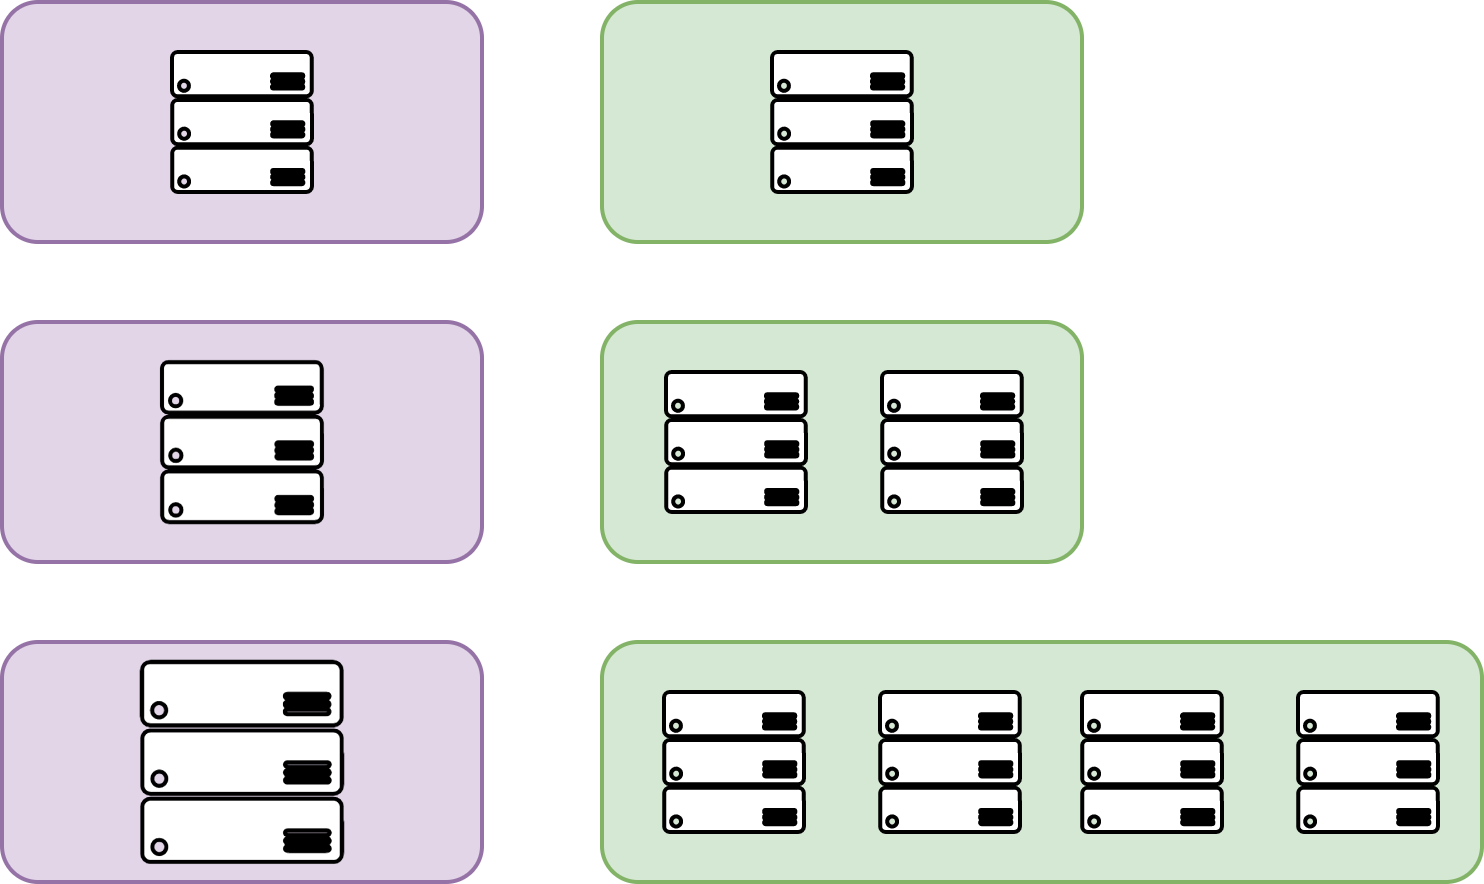
\includegraphics[scale=0.80]{images/Figure23}
	\end{center}
	\vspace{-0.6cm}
	\caption{Difference betweeen scaling vertically and horizontally}
	\label{fig:fig23}
\end{figure}

\noindent
Table~\ref{tab:table1} summarizes differences between horizontall and verticall scaling.

\begin{table}[h!]
	\begin{center}
		\begin{tabular}{l|l|l}
			\textbf{Feature} & \textbf{Scaling vertically} & \textbf{Scaling horizontally}\\
			\hline
			\textbf{Scaling} & Limited & Unlimited \\
			\textbf{Managment} & Easy & Comlex\\
			\textbf{Investments} & Expensive & Afordable \\
		\end{tabular}
	\end{center}
	\vspace{-0.5cm}
	\caption{Differences between horizontal and vertical scaling.}
	\label{tab:table1}
\end{table}

\noindent
Scaling horizontally is a preferable way for scaling DS. Not because we can scale easier, or because it is significantly cheaper than vertical scaling (after a certain threshold)~\cite{Bondi00}, but because this approach comes with few more benefits that are especially important when talking about large-scale DS. Adding more nodes gives us two important properties: 

\begin{itemize}
	\item \textbf{Fault tolerance} means that applications running on multiple places at the same time are not bound to the fail of a node, cluster, or even DCs. As long as there is a copy of the application running somewhere, the user will get a response back. As a consequence of running multiple copies of a service and on multiple places, we have that service is more \textbf{available}, than running on a single node no matter how high-end that node is. Eventually, all nodes are going to break, and if we have multiple copies of the same service we have a more resilient and more available system to serve user requests.
	\item \textbf{Low latency} refers to the idea that the world is limited by the speed of light. If a node running application is too far away, the user will wait too long for the response to get back. If the same application is running in multiple places, the user request will hit the node that is closest to the user.
\end{itemize}

\noindent
Nodes are usually organized into clusters of machines. Buyya et al. describes a cluster as a processing system, which consists of a collection of interconnected stand-alone computers cooperatively working together as a single, integrated computing resource.~\cite{Buyya}.

But despite all the obvious benefits, for a DS to work properly, we need the writing software in such a way that is able to run on multiple nodes, as well as that it \textbf{accepts the failure and deals with it}. This turns out to be not an easy task.

For example, users need to be aware when using DS which of them is related to distributed data storage systems. Storage implementations that rely on vertical scaling to ensure scalability and fault tolerance, have one nasty feature. 

This nasty feature is represented in theorem called \textbf{CAP theorem}~\label{lab:cap} presented by Eric Brewer~\cite{Brewer2000}, and proven after inspection by Gilbert et a.~\cite{GilbertL02}. The CAP theorem states that it is impossible for a distributed data store to simultaneously provide more than two out of three guarantees shown in Figure~\ref{fig:fig17}.

\begin{figure}[H]
	\begin{center}
		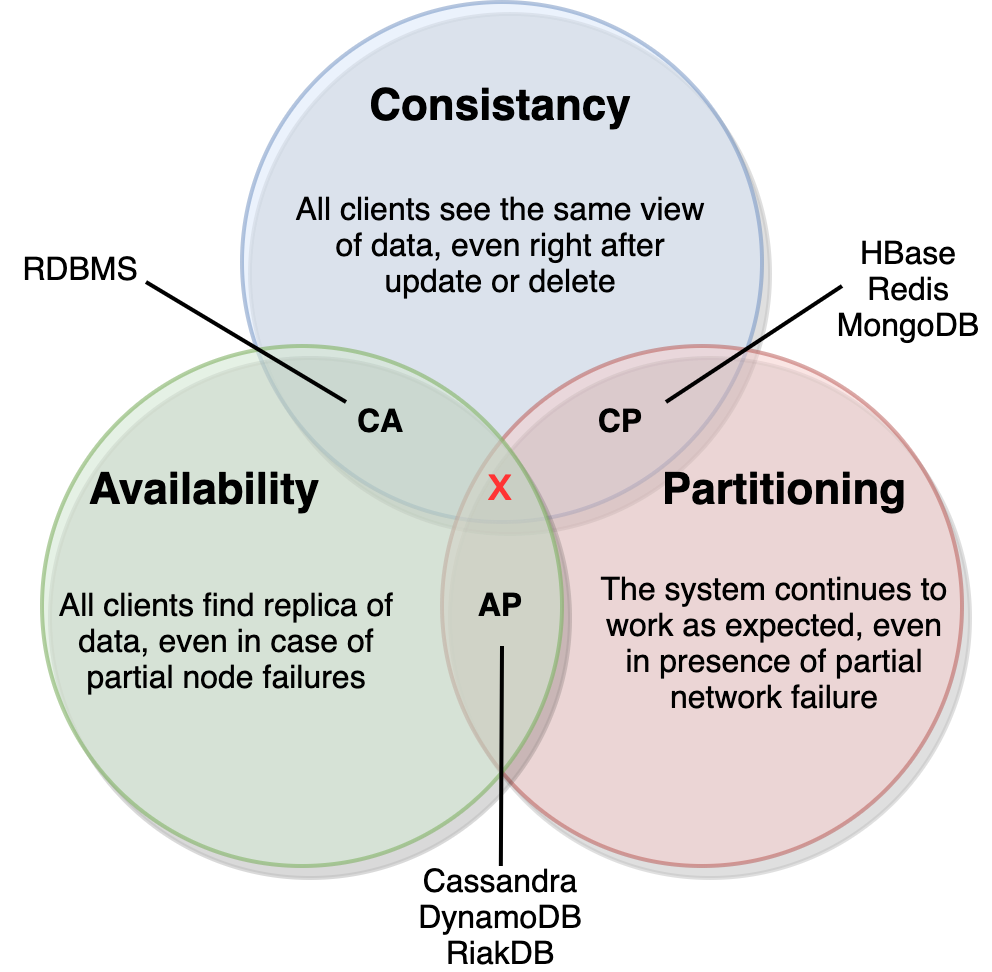
\includegraphics[scale=0.85]{images/Figure17}
	\end{center}
	\vspace{-0.6cm}
	\caption{Difference between cloud options and on-premises solution.}
	\label{fig:fig17}
\end{figure}

\begin{enumerate} [start=1,label={(\bfseries \arabic*)}]
	\item \textbf{C}onsistency, which means that all clients will see the same data at the same time, no matter which node they are connected to. Clients may not be connected to the same node since data could be replicated on many nodes in different locations.
	\item \textbf{A}vailability, which means that any client issued request will get a response back, even if one or more nodes are down. DS will not interpret this situation as an exception or error. Availability is represented in percentage, and it describes how much downtime is allowed per year. This can be calculated using formula:\\ 
	
	\begin{equation}\label{eq:Availability}
	Availability = \frac{uptime}{ (uptime + downtime)}
	\end{equation}
	\myequations{Availability percentage formula}
	The industry is using measuring availability in \say{class of nines}. Availability class is the number of leading nines in the availability figure for a system or module~\cite{GrayS91}. This metric relates to the amount of time (per year) that service is up and running. Table~\ref{tab:table7} show different classes of nine and their availability and unavailability in minutes per year (\textbf{min/year}) for some examples~\cite{GrayS91}.
	
	\begin{table}[h!]
		\begin{center}
			\begin{tabular}{l|l|l}
				\textbf{Type} & \textbf{Availability} & \textbf{Unavailability} \\
				\hline
				\textbf{Unmanaged} & 90\% & 50,000 \\
				\textbf{Managed} & 99\% & 5,000 \\
				\textbf{Well-managed} & 99.9\% & 500 \\
				\textbf{Well-managed} & 99.9\% & 500 \\
				\textbf{Fault-tolerant} & 99.99\% & 50 \\
				\textbf{High-availability} & 99.999\% & 5 \\
				\textbf{Very-high-availability} & 99.9999\% & 0.5 \\
			\end{tabular}
		\end{center}
		\vspace{-0.5cm}
		\caption{Downtime for different classes of nines.}
		\label{tab:table7}
	\end{table}
	
	\noindent
	We can calculate availability class if we have system availability $A$, the system's availability class is defined as~\cite{GrayS91}: 
	
	\begin{equation} 
	e^{\log_{10} \frac{1}{ (1 - A)}} 
	\end{equation}
	\myequations{Availability class formula.}
	It is important to notice that even a 99\% available system gives almost four days of downtime in a year, which is unacceptable for services like Facebook, Google, AWS, etc. And when the service is down, companies are losing customers.
	\item \textbf{P}artition tolerance, which means that the cluster must continue to work despite any number of communication breakdowns between nodes in the system. It is important to state that in a distributed system, partitions cannot be avoided.
\end{enumerate}

\noindent
Years after CAP theorem inception, Shapiro et al. prove that we can alleviate CAP theorem problems, but only in some cases, and offers \textbf{Strong Eventual Consistency (SEC) model}~\cite{ShapiroPBZ11}. They prove that if we can represent our data structure to be: \label{crdts}

\begin{itemize}
	\item \textbf{Commutative} $a*b = b*a$ \myequations{Commutative formula.}
	\item \textbf{Associative} $(a*b)*c = a*(b*c)$ \myequations{Associative formula.}
	\item \textbf{Idempotent} $(a * a) = a$ \myequations{Idempotent formula.}
\end{itemize}

\noindent
where $*$ is a binary operation, for example: $max$, $union$, $or$ we can rely on SEC properties,
%
%
\subsection{Cloud computing}\label{sec:cloud_computing}
%
Vogels et al. describe CC as an \say{aggregation of computing resources as a utility, and software as a service}~\cite{Vogels}.  Big DCs provide hardware and software services for their users over the internet~\cite{AboveTheCloud}. Cloud providers offer various resources like CPU, GPU, storage, and network as utilities that can be used and released on-demand~\cite{ZhangCB10}. 

The key strength of the CC is reflected in the offered services~\cite{Vogels}. To support the various application needs, the traditional CC model provides enormous computing and storage resources elastically. This property refers to the cloud ability to allow services to allocate additional resources or release unused ones to match the application workloads on-demand~\cite{AssuncaoVB18}. 

Services usually fall in one of three main categories: 

\begin{itemize}
	\item \textbf{Infrastructure as a service (IaaS)} allows businesses to purchase resources on-demand and as-needed instead of buying and managing hardware themselves;
	\item \textbf{Platform as a service (PaaS)} delivers a framework for developers to create, maintain and manage their applications. All resources are managed by the enterprise or a third-party vendor;
	\item \textbf{Software as a service (SaaS)} delivers applications over the internet to its users. These applications are managed by a third-party vendor;
\end{itemize}

\noindent
Figure~\ref{fig:fig1} shows the difference in control and management of resources between different cloud options and on-premises solutions.

\begin{figure}[H]
	\begin{center}
		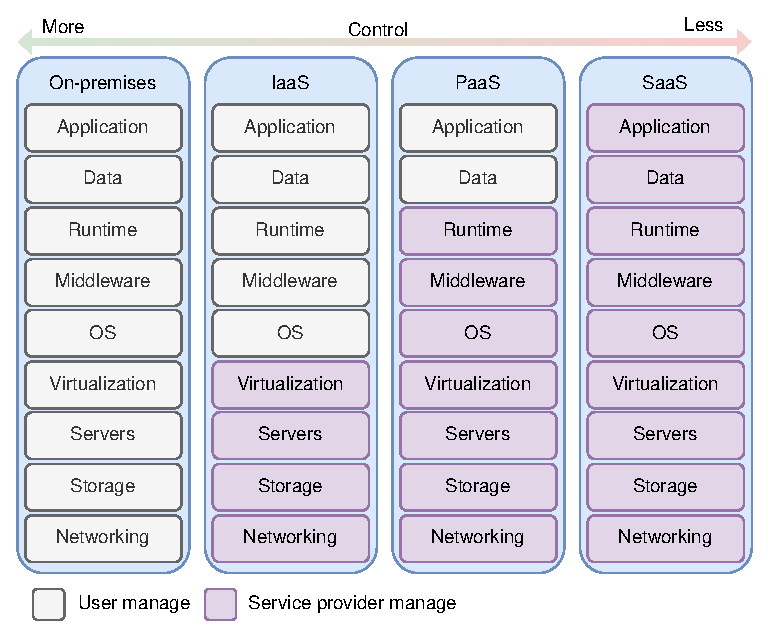
\includegraphics[scale=0.75]{images/Figure1}
	\end{center}
	\vspace{-0.6cm}
	\caption{Difference between cloud options and on-premises solution.}
	\label{fig:fig1}
\end{figure}

\noindent
The user can choose a single solution, or combine more of them if such a thing is required depending on preferences and needs.

By the ownership, CC can be categorized into three categories:

\begin{itemize}
	\item \textbf{Public cloud} is a type where CC is delivered over the internet and shared across many many organizations and users. In this type of CC, architecture is built and maintained by others. Users and organizations pay for what they use. Examples include AWS EC2, Google App Engine, Microsoft Azure, etc.
	\item \textbf{Private cloud} is a type where CC is dedicated only to a single organization. In this type of CC, architecture is built by an organization that may offer their solution or services to the users or other organizations. These services are in the domain of what the organization does, and that organization is in charge of maintenance. Examples include VMWare, XEN, KVM, etc.
	\item \textbf{Hybrid cloud} is such an environment that uses both public and private clouds. Examples include IBM, HP, VMWare vCloud, etc.
\end{itemize}

\noindent
Table~\ref{tab:table4} shows comparison of public, private and hybrid cloud capabilities.\label{sec_types}

\begin{table}[h!]
	\begin{center}
		\begin{tabular}{l|l|l|l}
			\textbf{Capabilities} & \textbf{Public cloud} & \textbf{Private cloud} & \textbf{Hybrid cloud}\\
			\hline
			\textbf{Data control} & IT enterprise & Service Provider & Both \\
			\textbf{Cost} & Low & High & Moderate \\
			\textbf{Data security} & Low & High & Moderate \\
			\textbf{Service levels} & IT specific & Provider specific & Aggregate \\
			\textbf{Scalability} & Very high & Limited & Very high \\	
			\textbf{Reliability} & Moderate & Very high & Medium/High\\	
			\textbf{Performance} & Low/Medium & Good & Good \\
		\end{tabular}
	\end{center}
	\vspace{-0.5cm}
	\caption{Comparison of public, private and hybrid cloud capabilities.}
	\label{tab:table4}
\end{table}

\noindent
In the rest of the thesis, if not stated differently when CC term is used it denotes public cloud.

CC has been the dominating tool in the past decade in various applications~\cite{Satyanarayanan17}. It is changing, evolving, and offering new types of services. Resources such as container as a service (CaaS), database as a service (DBaaS)~\cite{Peter} are newly introduced. The CC model gives us a few benefits. Centralization relies on the economy of scale to lower the cost of administration of big DCs. Organizations using cloud services avoid huge investments, like creating and maintaining their own DCs. They consume resources usually created by others~\cite{Satyanarayanan17} and pay for usage time -- pay as you go model. 

Centralization gives us a few really hard problems to solve. As already stated in section~\ref{sec:problem_area} data is required to be moved to the cloud from data sources, which introduces a high latency in the system~\cite{HossainRH18}. 

There are a few notable attempts to help data ingestion into the cloud. Remote Direct Memory Access (RDMA) protocol makes it possible to read data directly from the memory of one computer and write that data directly to the memory of another. This is done by using \textit{specialized hardware} interface cards and switches and software as well, and operations like read, write, send, receive, etc. do not go through the CPU. With these characteristics, RDMA has low latencies and overhead, and as such reaches better throughputs~\cite{CohenTKCKRCDG09}. This new hardware may not be cheap, and not every CC provider uses them for every use-case. This may not be enough, especially with the ever-growing amount of IoT devices and services.

Over the years there are more service options available, forming \textbf{everything as a service (XaaS)} model~\cite{DuanFZSNH15}. This model proposes that any hardware or software resource can be offered as a service to the users over the internet.

Table~\ref{tab:table2} shows common examples of SaaS, PaaS, and IaaS applications.

\begin{table}[h!]
	\begin{center}
		\begin{tabular}{l|l}
			\textbf{Platform} & \textbf{Common Examples}\\
			\hline
			\textbf{IaaS} & AWS, Microsoft Azure, Google Compute Engine \\
			\textbf{PaaS} & AWS Elastic Beanstalk, Azure, App Engine \\
			\textbf{SaaS} & Gmail, Dropbox, Salesforce, GoToMeeting \\
		\end{tabular}
	\end{center}
	\vspace{-0.5cm}
	\caption{Common examples of SaaS, PaaS, and IaaS.}
	\label{tab:table2}
\end{table}

\subsubsection{Multi-cloud and sky computing}
%
In recent years there has been one extension of CC from a series standpoint called \textbf{multi-cloud}~\cite{HongDSH19, Ardagna15} or sky computing~\cite{StoicaS21} (terms are going to be used interchangeably). 

It is such an environment where an enterprise uses more than one cloud platform, with at least two or more public cloud providers that each delivers a specific application or service. 

A multi-cloud can be comprised of any model presented on page~\pageref{sec_types}. This model relies on the possibility that if one cloud provider fails for whatever reason, the next one will be able to serve user requests.

This strategy allows creation of a single heterogeneous architecture, allowing distribution of cloud assets and workloads across multiple providers (active-active), or deploy a single workload on one provider, with a backup on another (active-passive)~\cite{Multicloud2019}.

CC gives a user an illusion that he is using a single machine, while the background implementation is fairly complicated and consists of various elements that are composed of countless machines. CC is a typical example of a horizontally scalable system presented in~\ref{sec:scalability}.
%
%
\subsection{Membership protocol}\label{sec:memership_protocol}
%
At the beginning of this section DS were introduced, and two interesting assumptions by Tanenbaum et al. were presented~\cite{SteenT16, 0019513}. If one more look is taken at~\ref{ds:asumption_2} assumption, we will see that users of the DS whether they are users or applications perceive DS as a single unit. Inside this single unit, nodes need to collaborate, so that they are able to do various kinds of tasks.

The most basic of all these tasks is that nodes need to know which group they belong to, and who are their peers in the group they will collaborate with. This might sound like a trivial idea, but when we include 8 fallacies of the DS~\ref{ds:8_fallacies} into the equation, things start to be not so trivial after all. In the setup where nodes are connected over the local network or internet, and they need to communicate, things will go wrong for various reasons.

To resolve the problem who their group peers are, a membership protocol comes to help. These protocols need to ensure that each process of one group updates its local list of \textbf{non-faulty} members of the group, and when a new process joins or leaves the group, the local list for every process needs to be updated. This is the most basic idea behind membership protocols.

Processes in the group of nodes in a group will ping each other in different ways, and using different strategies to figure out which nodes are dead and which are alive. There are a few existing algorithms that do this job, and they are (usually) based on the way epidemics spread or how gossip is spread in a human population. Because of this feature, these algorithms are usually called \textit{Gossip} style protocols.

Every membership protocol has some properties that will ensure efficiency and scalability:

\begin{enumerate}[start=1,label={(\bfseries \arabic*)}] \label{ds:features}
	\item \textbf{Completeness}, this property must ensure that every failure in the system is detected.
	\item \textbf{Accuracy}, in an ideal world, there should be no mistakes when detecting failures, but In a real-life scenario, we need to reduce false positives as much as we can.
	\item \textbf{Failure detection speed}, all failures needs to be treated as fast as possible, in order to remove the node from the group and reschedule the tasks from the dead node to alive ones.
	\item \textbf{Scale}, with this property we must ensure that the network load that is generated should be distributed equally between all processes in the group.
\end{enumerate}

\noindent
The easiest idea to implement this protocol would be \textbf{heartbeating} technique where process $P_i$ will send a heartbeat message to all his peers in the group or \textbf{multicast}. After some time if process $P_j$ did not receive a heartbeat message from $P_i$, it will mark him as failed. This idea is easy to understand, and implement but the downsides are that its process is not that \textbf{scalable}, especially for large groups, and this will introduce huge network traffic.

To resolve this problem, Das et al.~\cite{DasGM02} introduced \textbf{S}calable \textbf{W}eakly-consistent \textbf{I}nfection-style Process Group \textbf{M}embership protocol\newline (\textbf{SWIM} for short)\label{swim}. 
\noindent
This protocol divides the membership problem into two parts:

\begin{enumerate}[start=1,label={(\bfseries \arabic*)}]
	\item \textbf{Failure detection}, this component works so that one node will select a random node in the group, and it will send it $ping$ message, expecting $ack$ message in return --- \textbf{direct ping}. If such message is not received, it will pick $n$ nodes to probe through a $ping-req$ message --- \textbf{indirect ping}. If this fails, the node will be marked as $suspected$, and it will be marked as $dead$ after some timeout. If the node gets alive, it will ping some other node and it will get back into the group. Figure~\ref{fig:fig15} show message passing in \textbf{direct} $(left)$, and \textbf{indirect} $(right)$ ping in SWIM protocol.
	\item \textbf{Information dissemination}, with previous strategy, information can be disseminated by \textbf{piggybacking} the data on multiple messages ($ping$, $ping-req$ and $ack$), and avoid using the multicast solution.
\end{enumerate}

\begin{figure}[H]
	\begin{center}
		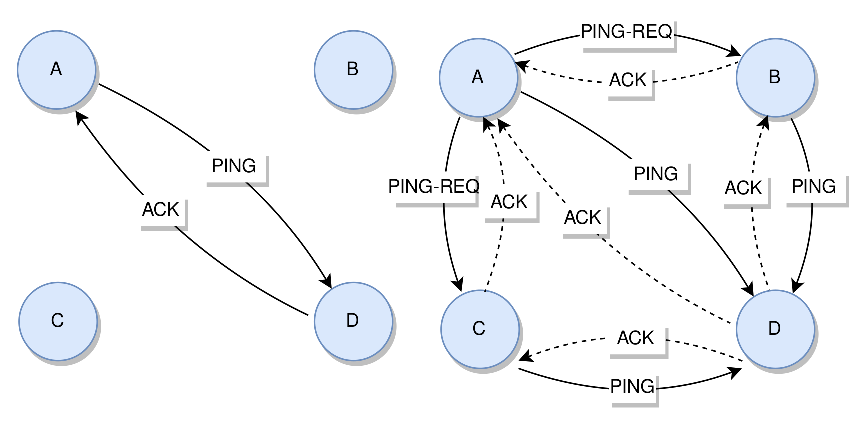
\includegraphics[scale=0.7]{images/Figure15}
	\end{center}
	\vspace{-0.6cm}
	\caption{Direct and indirect ping in SWIM protocol.}
	\label{fig:fig15}
\end{figure}

\noindent
Over the years, researchers found ways to improve the protocol, for example Dadgar et al. presented \textit{Lifeguard protocol}~\cite{DadgarPC18} for more accurate failure detection, and there are other implementations to fine-tune the SWIM, but the base idea is still there. Today SWIM or SWIM-like protocols are standard membership protocols whenever some node clustering is done.
%
%
\subsection{Mobile computing}\label{sec:mobile_computing}
%
The first idea that introduced task offloading from the cloud~\cite{FernandoLR13, LinLJL19} was Mobile cloud computing (MCC). Mobile devices run small client software and interact with the cloud over the internet, while heavy computation remains in the cloud. 

The cloud is usually far away from end devices because DCs are built on specific locations in the world to target as many users nearby as possible. This sparse deployment will most likely lead to high latency, and bad quality of experience (QoE)~\cite{LinLJL19} for most users. Latency-sensitive applications especially will have a hard time. As a model, MCC is not much different from the standard CC model. The good thing is that the cloud has been relaxed a little bit, and a small number of tasks has been moved from the cloud. But this model opens the door for the next-generation models.

The development led to new computing areas like EC, osmotic computig~\cite{VillariFDRJR19, VillariCF17}, sky computing~\cite{StoicaS21}, etc. EC is a next-generation model where computing and storage resources are in proximity to data sources~\cite{Satyanarayanan17}. This idea might overcome cloud latency issues and known MCC problems. The main strength of the EC lays in the CC enhancements with new processing ideas, for the next-generation use-cases~\cite{NingLSY20}. 

EC has brought a few different models over the years. Models like fog~\cite{BonomiMNZ14}, cloudlets~\cite{MonsalveCC18}, and mobile edge computing (MEC)~\cite{WangZZWYW17} emerged. This thesis will refer to all these models as edge nodes. Different EC models rely on the concept of data and computation offloading from the cloud closer to the ground~\cite{KhuneP19}. Only heavy computation remains in the cloud because of more available resources~\cite{NingLSY20}, compared to edge nodes. 

EC models introduced small-scale servers that operate between data sources and the cloud. These small-scale servers have much fewer capabilities compared to the cloud servers~\cite{ChenHLLW15}. To avoid latency and huge bandwidth~\cite{MonsalveCC18}, EC nodes can be dispersed in various locations, for example, base stations~\cite{WangZZWYW17}, coffee shops, or over arbitrary geographic regions.
%
%
\section{Distributed computing}\label{sec:distributed_computing}
%
Distributed computing (DC) can be defined as the use of a DS to solve one large problem by breaking it down into several smaller parts, where each part is computed in the individual node of the DS and coordination is done by passing messages to one another~\cite{0019513}. Computer programs that use this strategy and run on DS are called \textbf{distributed programs} \cite{Vera16, andrews2000foundations}. 

Similar to CC in Section~\ref{sec:cloud_computing}, to a normal user, DC systems appear as a single system similar to one the user uses every day on his/her personal computer. DC shares the same fallacies to DS presented in~\ref{sec:distributed_systems}.
%
%
\subsection{Big Data}\label{sec:big_data}
%
Term big data means that the data is unable to be handled, processed, or loaded into a single machine~\cite{FisherDCD12}. That means that traditional data mining methods or data analytics tools developed for centralized processing may not be able to be applied directly to big data~\cite{Tsai2015}. 

New tools and methods that have been developed rely on DS and one specific feature \textbf{data locality}~\label{ds:data_locality}. Data locality can be described as a process of moving the computation closer to the data, instead of moving large data to computation~\cite{GuoFZ12}. This simple idea minimizes network congestion and increases the overall throughput of the system.

Two examples of how huge generated data could be have already been given in~\ref{sec:problem_area}, and when other IoT sensors and devices are included these numbers will just keep getting bigger and bigger~\cite{SarigiannidisLR20}.

Contrary to relational databases that mostly deal with structured data, Big Data is dealing with various kinds of data~\cite{FisherDCD12, Tsai2015, GuoFZ12}:

\begin{itemize}
	\item \textbf{Structured} data is a kind of data that have some fixed structure and format. A typical example of this is data stored inside a table of some database. Organizations usually have no huge problem extracting some kind of value out of the data.
	\item \textbf{Unstructured} data is a kind of data where there is not any kind of structure at all. These data sources are heterogeneous and may contain a combination of simple text files, images, videos, etc. This type of data is usually in raw format, and organizations have a hard time deriving the value out.
	\item \textbf{Semi-structured} data is the kind of data that can contain both previously mentioned types of data. An example of this type of data is XML files.
\end{itemize}

\noindent
Along with the share size, big data have other instantly recognizable features called \textbf{V's} of big data~\cite{PatgiriA16}. 

The name is derived from initial letters of the other features that are describing big data. 

Image~\ref{fig:fig3} show 6 V's commonly used to represent the big data.

\begin{figure}[H]
	\begin{center}
		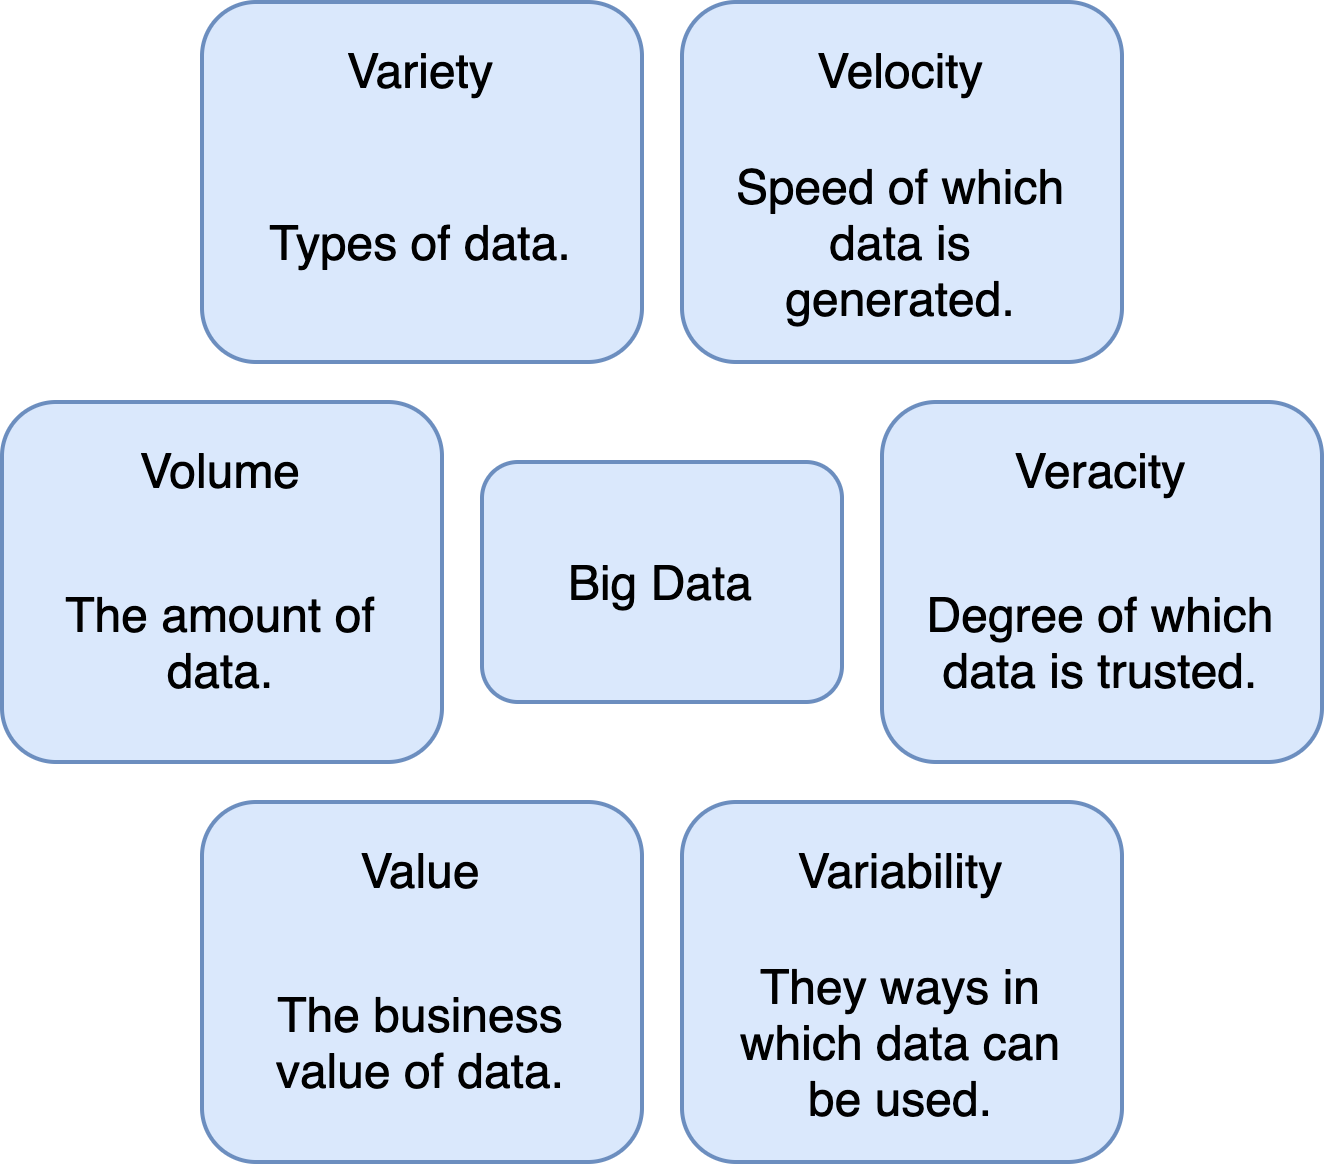
\includegraphics[scale=0.7]{images/Figure3}
	\end{center}
	\vspace{-0.6cm}
	\caption{V's of Big Data.}
	\label{fig:fig3}
\end{figure}

\noindent
Processing in big data systems can be represented as~\cite{phdthesis, KiranMMDB15}:

\begin{itemize}
	\item \textbf{Batch processing} represents a data processing technique that is done on a huge quantity of the stored data. This type of processing is usually slow and requires time.
	\item \textbf{Stream processing} represents a data processing technique that is done as data get into the system. This type of processing is usually done on a smaller quantity of the data \textbf{at the time}, and it is faster.
	\item \textbf{Lambda architectures} represents a processing technique where stream processing and handling of massive data volumes in a batch are combined in a uniform manner, reducing costs in the process~\cite{KiranMMDB15}.
\end{itemize}

\noindent
Big data systems, are not processing and value extracting systems. Big data systems can be separated into several categories: \textbf{(1)} data storage, \textbf{(2)}, data ingestion \textbf{(3)}, data processing, and analytics. All these systems aid to properly analyze ever-growing requirements~\cite{RaoMBG19},

Despite a promise that big data offers to derive value out of the collected data, this task is not easy to do and requires a properly set up system filtering and removing data that contains no value. To aid this idea, data could be filtered and a little bit preprocessed on close to the source~\cite{inproceedingsSimic1}, and as such sent to data lakes~\cite{MarynowskiSP15}.
%
%
\subsection{Microservices}\label{sec:microservices}
%
There is no single comprehensive definition of what a microservice is. Different people and organizations use different definitions to describe it. A working definition is offered in~\cite{DragoniGLMMMS16} as~\say{a microservice is a cohesive, independent process interacting via messages}. Despite the lack of a comprehensive definition, all agree on a few features that come with microservices:

\begin{enumerate}[start=1,label={(\bfseries \arabic*)}]
	\item they are small computer programs that are independently deployable and developed.
	\item they could be developed using different languages, principles, and using different databases.
	\item they communicate over the network to achieve some goal.
	\item they are organized around business capabilities~\cite{PautassoZALJ17}.
	\item they are implemented and maintained by a small team.
\end{enumerate}

'\noindent
The industry is migrating much of their applications to the cloud because CC offers to scale their computing resources per their usage~\cite{LiZJLZLGGS19}. Microservices are small loosely coupled services that follow UNIX philosophy~\say{do one thing and do it well}~\cite{krause2015microservices}, and they communicate over well defined API~\cite{DragoniGLMMMS16}.

This architecture pattern is well aligned to the CC paradigm~\cite{LiZJLZLGGS19}, contrary to previous models like monolith whose modules cannot be executed independently~\cite{DragoniGLMMMS16, abs-1905-07997}, and are not well aligned with the CC paradigm~\cite{abs-1905-07997}. Table~\ref{tab:table3} summarizes differences between the monolith and microservices architecture.

\begin{table}[h!]
	\begin{center}
		\begin{tabular}{l|l|l}
			\textbf{Feature} & \textbf{Monolith} & \textbf{Microservices}\\
			\hline
			\textbf{Structure} & Single unit & Independent services \\
			\textbf{Management} & Usually easier & Add DS complexity\\
			\textbf{Scale/Update} & Entire app & Per service \\
			\textbf{Error} & Usually crush entire app & App continue to work \\
		\end{tabular}
	\end{center}
	\vspace{-0.5cm}
	\caption{Differences between the monolith and microservices architecture.}
	\label{tab:table3}
\end{table}

\noindent
Since its inception, microservices architecture has gone through adaptations, and modern-day microservices are extended with two new models, each with its unique abilities and problems:

\begin{itemize}
	\item \textbf{Cloud-native applications} are specially designed applications for CC. They are distributed, elastic, and horizontally scalable systems by their nature, and composed of (micro)services that isolate state in a minimum of stateful components~\cite{KratzkeQ17}. These type of applications are self-contained, could be deployed independently, and they are composed of loosely coupled microservices that are packaged in lightweight containers. They have Improved resource utilization, and they are centered around APIs.
	\item \textbf{Serverless applications} is a computing model, where the developers need to worry only about the logic for processing client requests~\cite{AdzicC17}. Logic is represented as an event handler that only runs when a client request is received, and billing is done only when these functions are being executed~\cite{AdzicC17}. \textbf{Cold start} is one of the features of serverless computing, and we can define it as user requests need to wait until a new container instance is up and running before it can do any processing at all. Most providers have 1–3 second cold starts, and this is important for certain types of applications where latency is a concern. Cold start is only happening when there are no \textit{warm} containers available for the request, meaning there is no single instance to server request. Other features include: \textbf{(1)} simplified services development, \textbf{(2)} faster time to market, \textbf{(3)} and lower costs.
	\item \textbf{Service Mesh} is designed to standardize the runtime operations of applications~\cite{LiLGZH19}. As a part of the microservices ecosystem, this dedicated communication layer can provide several benefits, such as: \textbf{(1)} observability, \textbf{(2)} providing secure connections, or \textbf{(3)} automating retries and backoff for failed requests. With these features, developers only focus on the implementation of business logic, while operators gain out-of-the-box traffic policies, observability, and insights from the services. Advocates of the microservice movement, nowadays recommend using service mesh architecture when running microservices in production environments.
\end{itemize}

\noindent
Previous models are not explicitly different, they all can be viewed as cloud-native applications. The enumeration is given for the sake of pointing out their different models and aspects of working.

Microservices communicate over a network to fulfill some goal using message passing techniques and technology-agnostic protocols such as HTTP. They can be implemented as:

\begin{itemize}
	\item Representational state transfer (REST) services~\cite{AdamczykSJH11}, is an architectural style with a set of constraints that users can create web services and interoperability between computer systems on the internet. It is based on HTTP routs to define resources and use HTTP verbs to represent operations over these resources. It relies on textual based communications, and payload could be represented using $JSON$, $XML$, $HTML$ etc.
	\item Remote procedure calls (RPC) represent an architectural way to design services that can call subroutines that are located in different places, usually on another machine. The client calls these operations like they are located locally in his address space.
	\item Event-driven services are services where communication between services is done using events. Events are sent on some channel and other read messages that are received on another channel. These channels could be implemented either like message queues or message topics. Services connect to message queue or subscribe to the specific topic, and when messages arrive, they can act according to the message type.
\end{itemize}

\noindent
They are well aligned with text-based protocols like HTTP/1 using $JSON$ for example, or binary protocols such as HTTP/2 using $protobuf$ and $gRPC$ for example, and even new faster version like HTTP/3 over new $QUIC$ protocol, designed by Google. HTTP 3 is the latest version of the conventional and trusted HTTP protocol. It is very similar to HTTP 2, but it also offers a few important new features. 

Table~\ref{tab:table9} shows important difference between versions of HTTP protocol.

\begin{table}[h!]
	\begin{center}
		\begin{tabular}{l|l|l|l}
			\textbf{Feature} & \textbf{HTTP1} & \textbf{HTTP2} & \textbf{HTTP3}\\
			\hline
			\textbf{Transport} & text & binary & binary\\
			\textbf{Parallelism} & No & Yes & Yes\\
			\textbf{Protocol} & TCP & TCP & QUIC \\
			\textbf{Space} & OS level & OS level & User level\\
			\textbf{Server push} & No & Yes & Yes\\
			\textbf{Compression} & Data & Data/Headers & Data/Headers\\
		\end{tabular}
	\end{center}
	\vspace{-0.5cm}
	\caption{Idempotent and non-idempotent operations.}
	\label{tab:table9}
\end{table}

\noindent
To ensure a wider range of devices that can communicate with the rest of the systems, developers usually have a gateway into the system that is REST service, and other services could be implemented differently.

It is important to point out, that all flavors of microservices applications rely on continuous delivery and deployment~\cite{7436659}. This is enabled by lightweight containers, instead of virtual machines~\cite{FelterFRR15}, and orchestration tools such Kubernetes~\cite{BurnsGOBW16}. These concepts will be described in more detail in Section~\ref{sec:virtualization_techniques}.

Microservices architecture is a good starting point especially for being built as a service applications model, and applications that should serve a huge amount of requests and users, especially with the benefits of CC to pay for usage, and the ability to scale parts of the system independently.  They are not necessarily easy to implement properly, and there is more and more critique to the architecture model~\cite{SoldaniTH18}. Microservices are rely upon and use parts of the DS, and as such, they inherit almost all problems DS has. 

One particular thing that users need to be aware of is \textbf{idempotency}. In microservices applications, developers are dealing with inconsistencies in the distributed state, and their operations should be implemented as idempotent. An operation is idempotent if it will produce the same results when executed over and over again. It is a strategy that means that operations with side effects like creation or deletion can be called any number of times while guaranteeing that side effects only occur once. Idempotency is a term that comes from mathematics, and can be represented by simple idempotency law for operation $*$ like~\cite{gratzer2002general}:

\begin{equation}\label{form:idempotency_law}
\forall x, x * x = x
\end{equation}
\myequations{Idempotency law formula}

\noindent
Not all Create, Read, Update, Delete (CRUD) operations are idempotent by default. Developers need to make effort to make all of them idempotent, to prevent bad outcomes and inconsistent states. 

Table~\ref{tab:table8} shows list of idempotent and non-idempotent for standard CRUD operations:

\begin{table}[h!]
	\begin{center}
		\begin{tabular}{l|c|c}
			\textbf{Operation} & \textbf{Idempotent} & \textbf{Non-idempotent}\\
			\hline
			\textbf{Create} &  & x \\
			\textbf{Read} & x & \\
			\textbf{Update} & x & \\
			\textbf{Delete} & x & \\
		\end{tabular}
	\end{center}
	\vspace{-0.5cm}
	\caption{Idempotent and non-idempotent operations.}
	\label{tab:table8}
\end{table}

\noindent
\emph{Crate} operation is \textbf{not} idempotent by default, but to make it idempotent there are multiple strategies how to do so. The most common way is to create \textbf{idempotency key} that will be sent in the request, and based on that request server can decide if this operation is already invoked or not. If a server has already \say{seen} specified idempotency key than the operation is already done and we can return just the response that the operation is done but no operation will be done over the state of the service or application. If the server sees the idempotency key for the first time, that is the signal that this request is a new one, and it should be done.

Idempotency key could be stored in any kind of storage, it is not uncommon that these keys are stored in cache storage with some time to live (TTL) policy that will automatically remove the key after a specified time.

Another option that is commonly used is hashing user specified actions. It is useful to know which part of the action set is already done and which is not. This strategy is used in scenarios where we must preserve the order of actions.
%
%
\subsubsection{Distributed Queries}
%
Applications built using microservices architecture propose different strategies for data storage. One common and recommended technique is \emph{database per service} patter~\cite{richardson2018microservices}.

The result of this technique is that overall state of the system will be distributed across multiple data stores, accessible only from their own microservices. This creates two important topics to think about: \textbf{(1)} transactions that span over multiple services can be implemented using \emph{Sagas} for example (cf.~\pageref{sec:sagas})
, and \textbf{(2)} the complex queries which require data from multiple databases.

The complex queries will involve data available in multiple databases, and a client can access all these microservices and aggregate data, however, this is not the recommended solution because the client does not have full understanding how the system manages the data.

In microservices archtiecture, there are two standard ways to solve this problem~\cite{richardson2018microservices}:

\begin{enumerate}
	\item \textbf{Command Query Responsibility Segregation (CQRS)}\label{par:cqrs} separates responsibility for \emph{modifying} data (command), and \emph{reading} the data (query), making the logic clearer and easier to optimize different parts of the system~\cite{richardson2018microservices, 8101372}. This increases the complexity of entire system, but it supports multiple denormalized views that are scalable and performant~\cite{richardson2018microservices}. 
	
	When the data in one service is modified, the service emits the event, which will change the service responsible for complex query. The service that will serve the queries will keep the \emph{read-only} replica of the data. 
	
	Figure~\ref{fig:fig21} shows an example diagram for CQRS pattern.
	
	\begin{figure}[H]
		\begin{center}
			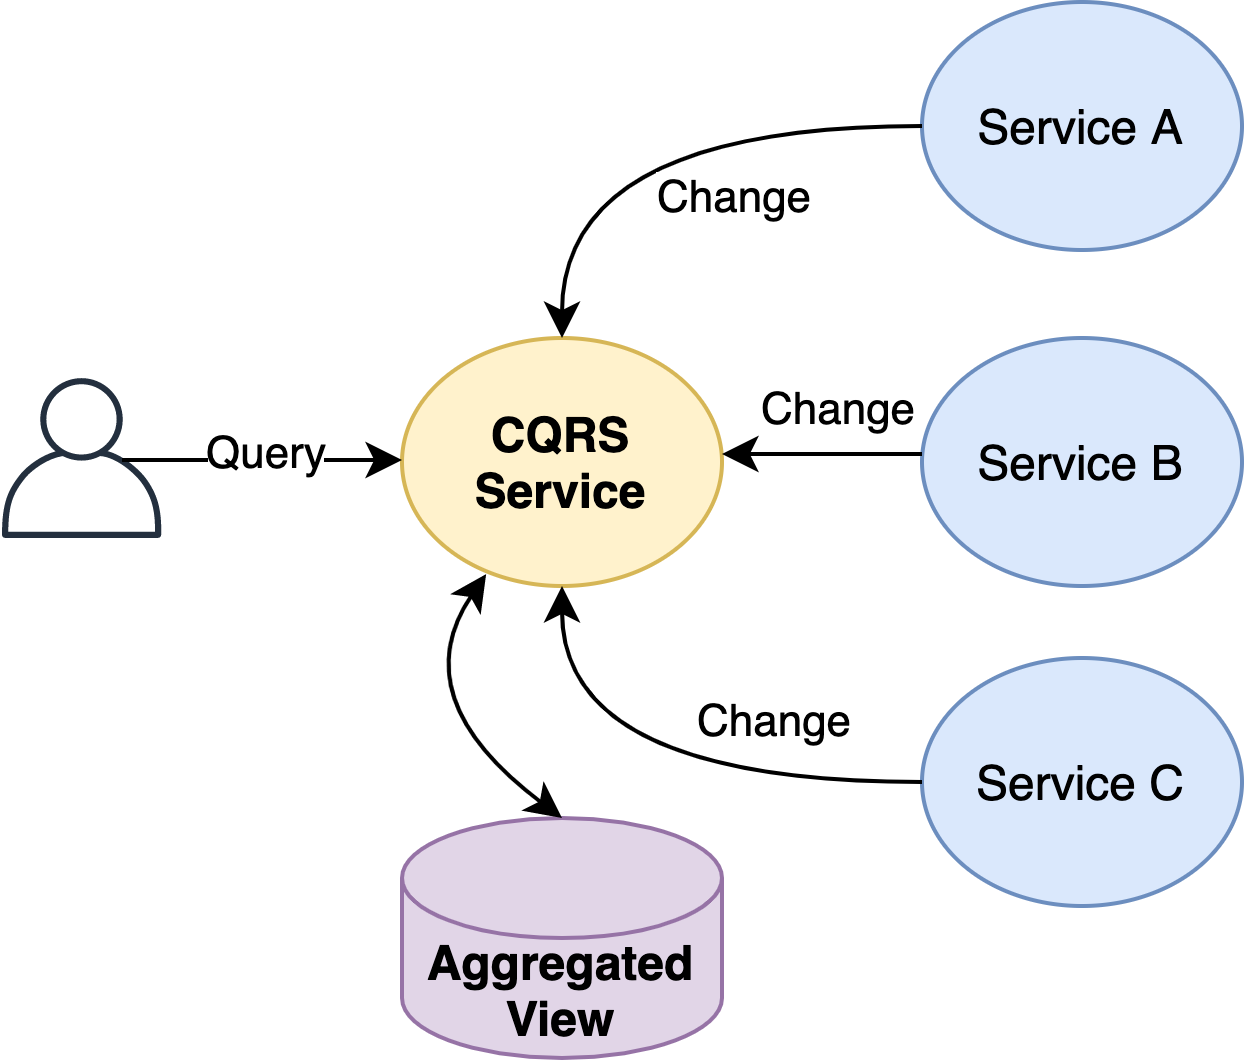
\includegraphics[scale=0.7]{images/Figure21}
		\end{center}
		\vspace{-0.6cm}
		\caption{CQRS pattern diagram.}
		\label{fig:fig21}
	\end{figure}

	\item \textbf{API composition}\label{par:composition} is a simple way to query data in a microservice architecture~\cite{richardson2018microservices, 8890660}, alternative and more lightweight solution than CQRS. 
	
	The main difference between CQRS is that this patterns does not have its own data storage. When a request comes in, it accesses every single microservice containing data, combines the results, and then returns the combined result to client. Making it easier to implement, because database does not need to be refreshed every time when some change occurs in the system. On the other hand, it may yield a slower response, depending on how many services we need to contact for the information, their availability, and time to merge and prepare data in memory. 

	Figure~\ref{fig:fig22} shows an example diagram for API Compossition pattern.

	\begin{figure}[H]
		\begin{center}
			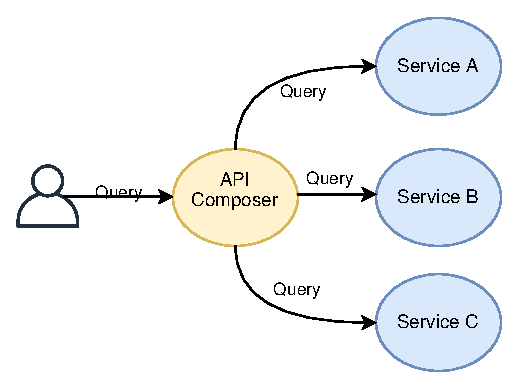
\includegraphics[scale=0.7]{images/Figure22}
		\end{center}
		\vspace{-0.6cm}
		\caption{API Compossition pattern diagram.}
		\label{fig:fig22}
	\end{figure}
\end{enumerate}

The best chance to succeed when implementing a microservices architecture is to simply follow existing patterns and use existing solutions with proven quality. 
%
%
\subsection{Observability}\label{sec:log_aggregation}
%
Observability is an integral part of any real-world computing system, and especially in the DS where observing what is happening in a network of processes is difficult~\cite{Fidge96}, due to the its nature.

In case of errors, fails or misbehavior of the system, some insight can be gained into what causes failure or which set of parameters in which circumstances. The three pillars of the observability are: \textbf{(1)} logs aggregation, \textbf{(2)} distributed tracing, and \textbf{(3)} alerting.

The logging operation, gives developers ability to store various arbitrary informations, that will provide more details for those who are investigating the failure. One thing we must be aware of is not to store any sensitive pieces of information in the log because this can cause a bunch of problems. Another thing we must be aware of is that we do not log too much and too often to slow down the business logic and execution of the function.

In monolithic applications logging and monitoring is a little bit easier to implement, because we have the whole application state in one place. When we come to the field of DS and microservices, our state is scattered across multiple elements or services. In DS, the monitoring involves interactions among concurrently executing processes~\cite{JoyceLSU87}.

The solution to this problem is to use a centralized logging service -- \textbf{logs aggregation}, that collects logs from each service~\cite{BeschastnikhWBE16}. This is beneficial because users can search and analyze the logs as a whole state of the system. To do this properly the log must be stored very reliably~\cite{DanielsST87}. Users can then configure the log server for some alerts that are triggered when certain messages appear in the logs. The log of DS usually does not contain enough information to regenerate the timeline of execution, and this is one reason that logs in DS are so hard to interpret~\cite{BeschastnikhWBE16}.

To resolve this problem of DS execution timeline, Google develops a new technique called \textbf{tracing}~\cite{36356}. The trace represents a single execution timeline or execution of one request. Trace will create a tree, and the tree is used to establish order. Every node in the tree represents a unit of work and it is called span. A tree unites all the elements needed to carry out an originating request. In every span or unit of work, we can attach more details about that particular execution element. 

Figure~\ref{fig:fig18} shows the simple example of \textit{RequestX} path through the processes in a distributed system, where each service \textbf{call} could be RPC, HTTP or some other request.

\begin{figure}[H]
	\begin{center}
		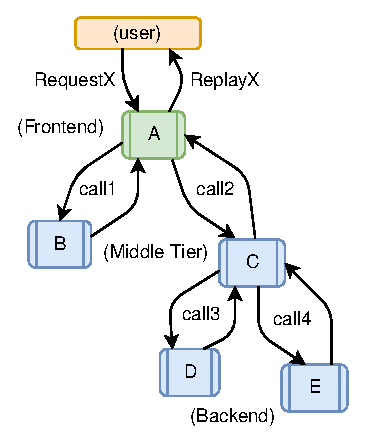
\includegraphics[scale=0.8]{images/Figure18}
	\end{center}
	\vspace{-0.9cm}
	\caption{\textit{RequestX} path through the processes in a distributed system.}
	\label{fig:fig18}
\end{figure}

\noindent
And last, but not the least option is \textbf{alerting}. Alerting of a monitored system can be represented as a set of rules that performs actions based on changes in specific metric. Alerting enables a system to notify users when something important happens or (probably) is going to happen.

DS logging, tracing and alerting represents the important role of any system, and as such, it should not be neglected especially in the DS environment. Every user request should be traced and logged from an infrastructure perspective, but we should allow users to store logs from their applications.
%
%
\section{Distribution Models}\label{sec:distribution_models}
%
The role of distribution models is to determine the responsibility for the request, or to answer the fundamental question \say{who is in charge} for a specific request. There are two ways to answer this question: \textbf{(1)} all nodes in the system, or \textbf{(2)} single node in the system.
%
%
\subsection{Peer-to-peer}\label{sec:p2p_networks}
%
Peer-to-peer (P2P) communication is a networking architecture model that partitions tasks or workloads between peers~\cite{Schollmeier01}. All peers are created equally in the system, and there is no such thing as a node that is more important than others. 

Every Peer has a portion of system resources, such as processing power, disk storage, or network bandwidth, directly available to other network participants, without the need for central coordination by servers or stable hosts~\cite{Schollmeier01}. P2P nodes are connected and share resources without going through a separate server computer that is responsible for routing. 

Figure~\ref{fig:fig2} shows difference in network topology between P2P networks $(left)$ and client-server architecture $(right)$.

\begin{figure}[H]
	\begin{center}
		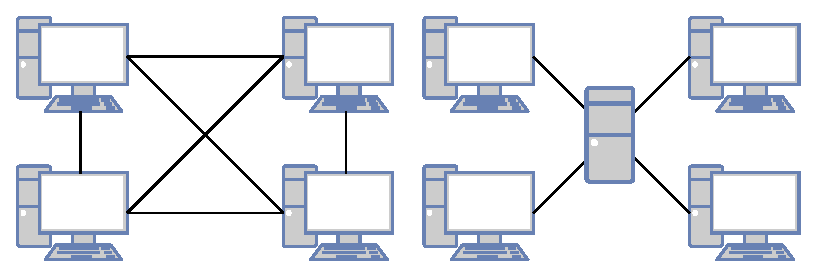
\includegraphics[scale=0.6]{images/Figure2}
	\end{center}
	\vspace{-0.6cm}
	\caption{P2P network and client-server network.}
	\label{fig:fig2}
\end{figure}

\noindent
Peers are creating a sense of virtual community. This community of peers can resolve greater tasks, beyond those that individual peers can do. Yet, these tasks are beneficial to all the peers in the system~\cite{BandaraJ13}. When a request comes to such a network, a node that accepts the request is usually called \textbf{coordinator}, because it then is trying to find the right peer to send a request to.

Based on how the nodes are linked to each other within the overlay network, and how resources are indexed and located, we can classify networks as~\cite{KamelSE07}:

\begin{itemize}
	\item \textbf{Unstructured} do not have a particular structure by design, but they are formed by nodes that randomly form connections~\cite{FilaliBHB11}. Their strength and weakness at the same time is the lack of structure. These networks are robust when peers join and leave the network. But when doing a query, they must find more possible peers that have the same piece of data. A typical example of this group is a Gossip-based protocol like~\cite{DasGM02}.
	\item \textbf{Structured} peers are organized into a specific topology, and the protocol ensures that any node can efficiently search the network for a resource. The famous type of structured P2P network is a Distributed Hash Table (DHT). These networks maintain lists of neighbors to do a more efficient lookup, and as such, they are not so robust when nodes join or leave the network. DHT is commonly used in resource lookup systems~\cite{StoicaMKKB01}, and as efficient resource lookup management and scheduling of applications, or as an integral part of distributed storage systems and NoSQL\cite{Leavitt10} databases.
	\item \textbf{Hybrid} combine the previous two models in various ways.
\end{itemize}

\noindent
P2P networks are a great tool in many arsenals, but because of their unique ability to act as a server and as a client at the same time, we must be careful and pay more attention to security because they are more vulnerable to exploits~\cite{0024003}.
%
%
\subsection{Master-slave}\label{sec:master_slave}
%
In the master-slave architecture, there is one node that is in charge -- \textbf{master}. This node accepts requests, and we usually do not communicate to the rest of the nodes or \textbf{slaves}. The master node is usually better and more expensive or even specialized hardware such as redundant array of inexpensive disks (RAID) to lower the crash probability. The cluster can also be configured with a \textbf{standby} master, and this node is continually updated from the master node.

But no matter how specialized hardware master runs on, it is prone to fail for various reasons, so it is a \textbf{single point of failure (SPOF)}. If crush happens, then standby master could continues to the server as a master, or new \textbf{leader election} protocol~\cite{KorachKM90} is initiated to pick a new master node. 

The master node is responsible for processing any updates to that data. If the master fails, then the slaves can still handle \textbf{read} requests. Failure of the standby master node to take over from the master node is a real problem if we want to achieve a high-availability system.

Figure~\ref{fig:fig16} shows difference between mater-slave $(left)$ and peer-to-peer $(right)$ request handling.

\begin{figure}[H]
	\begin{center}
		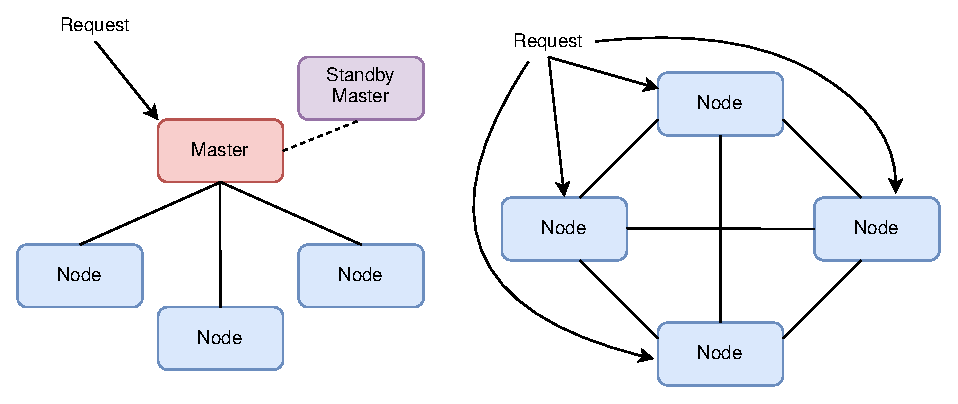
\includegraphics[scale=0.6]{images/Figure16}
	\end{center}
	\vspace{-0.6cm}
	\caption{Handling requests master-slave and peer-to-peer}
	\label{fig:fig16}
\end{figure}

\noindent
Using the right distribution model usually depends on the business requirements. High availability requires a P2P network because of no SPOF. If we could manage data using batch jobs that run in off-hours, then the simpler master-slave model might be the solution.
%
%
\section{Similar computing models}\label{sec:similar_models}
%
In this section, we are going to shortly describe models that are similar to the DS, and as such, they may be the source of confusion.
%
%
\subsection{Parallel computing}\label{sec:parallel_computing}
%
DC and parallel computing seem like models that are the same, and that may share some features like simultaneously executing a set of computations in parallel. Broadly speaking, this is not far from the truth~\cite{Vera16}. 

Differencies between the two can be presented as follows: in parallel computing, all processor units have access to the shared memory and have some way of the faster inter-process communication, while in DS and DC all processors have their memory on their machine and communicate over the network to other nodes which are significantly slower. 

These models are similar, but they are not identical, and the kinds of problems they are designed to work on are different. Figure~\ref{fig:fig4} visually summarizes the architectural  differences between DC $(up)$ and parallel computing $(down)$.

\begin{figure}[H]
	\begin{center}
		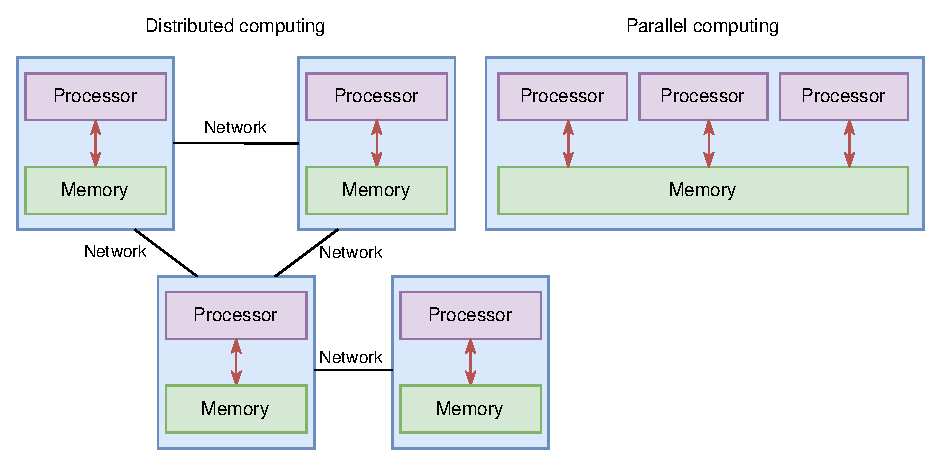
\includegraphics[scale=0.6]{images/Figure4}
	\end{center}
	\vspace{-0.6cm}
	\caption{Architectural difference between DC and parallel computing.}
	\label{fig:fig4}
\end{figure}

\noindent
Parallel computing has often used the strategy with problems that due to their nature or constraints must be done on multi-core machines simultaneously~\cite{0072397}. It is often that some big problems are divided into smaller ones, which can then be solved at the same time. 

Several tasks require parallel computing like simulations, computer graphics rendering, or different scenarios in scientific computing.
%
%
\subsection{Decentralized systems}\label{sec:decentralized_systems}
%
Decentralized systems are similar to DS, in a technical sense, they are still DS. But if we take a closer look, these systems \textbf{should not} be owned by a single entity. CC, for example, is a perfect example of DS, but it is not decentralized by its nature. It is a centralized system by the owner like AWS, Google, Microsoft, or some other private company because all computation needs to be moved to big DCs~\cite{HossainRH18}.

By modern standards, when we are talk about decentralized systems, we usually think of blockchain or blockchain-like technology~\cite{LeibleSSG19}, since here we have distributed nodes, that are scattered and there is no single entity that owns all these nodes. But even if this technology is run in the cloud, it is loses the decentralized feature. This is the caveat we need to be aware of. These systems are facing different issues because any participant in the system might be malicious and they need to handle this case. 

Nonetheless, CC can and should be decentralized in the sense that some computation can happen outside of cloud big DCs, closer to the sources of data. These computations could be owned by someone else, and big cloud companies could give their solution to this as well to relax centralization and problems that CC will have especially with ever-growing IoT and mobile devices.
%
%
\section{Transactions}\label{sec:transactions}
%
Transactions are keeping data consistent even in the presence of highly concurrent data accesses and despite all sorts of failures~\cite{WeikumV2002}. Transactions are trying to resolve this problem in a generic way, in such a way that is invisible to the application logic.

The main goal of transactions is to maintain system integrity in the consistent state, by ensuring that all operations on the system are either all completed successfully or all canceled successfully. Transactions are typically used in systems that needs to preserve some state (e.g. database or some filesystems). 

In their book Gray et al. make a good parallel with the contract law, saying that transactions give us the ability to \emph{clean up the situation}, if something does not work right.~\cite{GrayR93}.

Transactions guarantee following four properties: \textbf{(1)} atomicity, \textbf{(2)} consistency, \textbf{(3)} isolation, and \textbf{(4)} durability, also known as \emph{ACID} properties.
%
%
\subsection{Distributed transactions}\label{sec:distributed_transactions}
%
Because of the nature of DS, more network hosts are involved which significantly complicates the transaction mechanism. Distributed transactions are required to have all four \emph{ACID} properties. This might not be so easy to achieve amongst other due to \emph{CAP} theorem~\pageref{lab:cap}. 

In their book, Morgan et al. claim that here exists no distributed commit protocol that can guarantee independent process recovery in the presence of multiple failures (e.g., network partitionings)~\cite{WeikumV2002}.

Distributed transactions include few protocols such as two-phase commit (2PC), three-phase commit (3PC), Paxos, and various other approaches to quorum giving programmers facade of global serializability~\cite{Helland07}. 

Avoiding distributed transactions allows a much simpler, more robust and efficient solution.
%
%
\subsection{Sagas}\label{sec:sagas}
%
In 1987, Molina et al. presented \emph{Sagas}~\cite{Garcia-MolinaS87} and their work in the area of \emph{long-lived transactions (LLTs)}, types of transactions that hold resources for long periods, and as such delay shorter and more common transactions. 

These transactions are increasingly relevant and important, in the current technological landscape with the distribution of components and microservices architectures.

The saga transaction is composed of sub-transactions, executed in an atomic way so that either all or none of the sub-transactions take effect. However, no isolation is necessarily guaranteed between the sub-transactions of different sagas.

One transaction $T$ is composed of multiple sub-transactions $T_1,\ldots,T_n$, and every sub-transaction $T_i$ has an associated \emph{compensating transaction} $C_i$ or how the effects of the transaction can be rolled back. The saga transaction executes sub-transactions sequentially.

Figure~\ref{fig:fig20} shows an example of one transaction separated into multiple sub-transactions where \emph{green} arrows represent success path, while \emph{red} arrows represent rollbacks, structure of the saga transaction and at least the previous and next element in the chain.

\begin{figure}[H]
	\begin{center}
		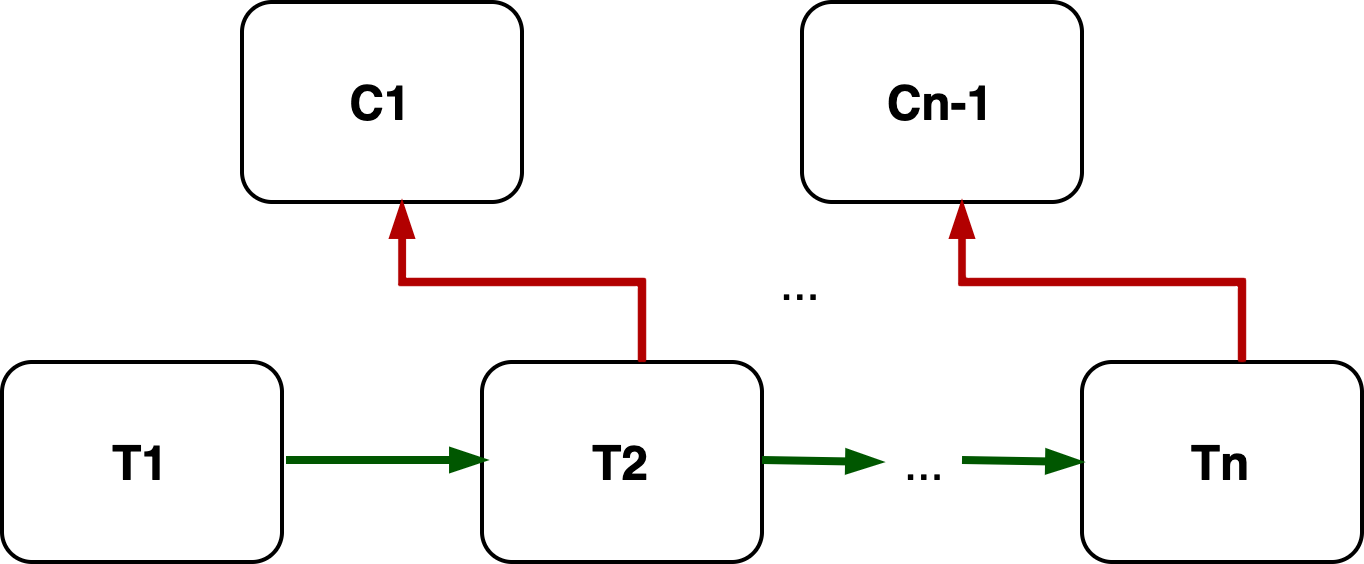
\includegraphics[scale=0.9]{images/Figure20}
	\end{center}
	\vspace{-0.6cm}
	\caption{Saga transactions separated in sub-transactions.}
	\label{fig:fig20}
\end{figure}

\noindent
Sagas can be implemented using two patterns: \textbf{(1)} orchestration where one centralized element is responsible for all the coordinating, or \textbf{(2)} choreography, where each service trigger local transactions in other services.

This isolation can be added in the application layer~\cite{Frank}l for example using \emph{semantic lock}. This strategy will change state so that some data are in process and should be treated differently. 

For example, an order can be in one of the following states: \textbf{(1)} \emph{PENDING}, \textbf{(2)} \emph{COMPLETED}, or \textbf{(3)} \emph{CANCELED} state. Other transactions will not make use the data if status is not set to \emph{COMPLETED}.
%
%
\section{Garbage collection}\label{sec:garbage_collection}
%
Most modern programming languages nowadays allow programmers to allocate and free memory. This process can be in total responsibility of the programmer, or language can handle this process for the programmer. When there is some automatic process involved to release unused resources, that process is called \textbf{garbage colection} or GC. 

In~\cite{JonesL96}, Jones, et al. describe \emph{garbage collection} as the automatic management of dynamically allocated storage. However, the term \emph{garbage collection} is not exclusive to programming languages. It is widely used to refer to all forms of automatic management of dynamically allocated resources.

Even with the rapid growth of memory sizes, and lowering the overall cost of memory is not inexhaustible. Like any other limited resources, it requires careful consideration and recycling. Even tools like Kubernetes, have some form of garbage collection that is used to remove unused items and their references in the system.

Over the years, different algorithms are used to do reference counting and tracing methods, to discover unused resources, and to free them. One of the most common algorithms for garbage collection is \emph{mark-sweep} algorithm~\cite{McCarthy60} developed in 1960. The variety on the topic exists today, but the essence of the algorithm remains widely used today.

Traditional automated garbage collection is usually seen as slow, and disruptive to executing programs. Modern implementations of the garbage collection substantially reduced the overhead of the system~\cite{JonesL96}.
%
%
\section{Virtualization techniques}\label{sec:virtualization_techniques}
%
Virtualization as a technique started long ago in time-sharing systems, to provide isolation between multiple users sharing a single system like a mainframe computer~\cite{CrosbyB06}. 

In~\cite{Sharma} Sharma et al. virtualization is described as technologies that provide a layer of abstraction of the physical computing resources between computer hardware systems and the software systems running on them.

Modern virtualization differentiates several different tools. Some of them are used as an integral part of the infrastructure for some flavors like IaaS, while others are used in different CC flavors as well as microservices packaging and distribution format, or are new and still are looking for their place. These options are:

\begin{itemize}
	\item \textbf{Virtual machines (VM)} are the oldest technology of the three. They are described as a self-contained operating environment consisting of guest operating system and associated applications, but independent of the host operating system~\cite{Sharma}. VMs enable us to pack isolation and better utilization of hardware in big DCs. They are widely used in IaaS environment~\cite{AbsalomBJ13, YangHCLW13} as a base where users can install their own operating system (OS) and require software tools and applications.
	\item \textbf{Containers} provide the almost same functionality to VMs, but there are several subtle differences that make them a go-to tool in modern development. Instead of the guest OS running on top of host OS, containers use tools that are in a Linux kernel like \textit{cgroups} that limit process resource usage so that single process can not starve other processes and use all the resources for itself, and \textit{namespaces} to provide isolation and partitions kernel resources so that single process sees node resources like it only exists there. Containers reduce time and footprint from development to testing to production, and they utilize even more hardware resources compared to VMs and show better performance compared to the VMs~\cite{Seo2014PerformanceCA, FelterFRR15}. Containers provide an easier way to pack services and deploy and they are especially used in microservices architecture and service orchestration tools like Kubernetes~\cite{BurnsGOBW16}. Google has stated several times in their online talks that they have used container technology for all their services, they even run VMs inside containers for their cloud platform. Even though they exist for a while, containers get popularized when companies like Docker and CoreOS developed user-friendly APIs.
	\item \textbf{Unikernels} is the newest addition to the virtualization space. Unikernels are defined as small, fast, secure virtual machines that lack operating systems~\cite{pavlicek2016unikernels}. Unikernels are comprised of source code, along with only the required system calls and drivers. Because of their specific design, they have a single process and they contain and execute what it absolutely needs to nothing more and nothing less~\cite{GoethalsSAVT18}. They are advertised as new technology that will save resources and that they are \textit{green}~\cite{208735}, meaning they save both power and money. When put to the test and compared to containers they give interesting results~\cite{GoethalsSAVT18, PlauthFP17}. Unikernels are still a new technology and they are not widely adopted yet. But they give promising features for the future, especially \textbf{if} properly ported to ARM architectures, and various development languages. Unikernels will probably be used as a user application and function virtualization tool, because of their specific architecture, especially for serverless applications presented in~\ref{sec:microservices}.
\end{itemize}

\noindent
With every virtualization technique, the ultimate goal is to pack as many applications on existing hardware as possible, so that there are no resources that are left not used -- we are trying to achieve high resource utilization. 

Figure~\ref{fig:fig5} represents architectural differences between VMs, containers, and unikernels.

\begin{figure}[H]
	\begin{center}
		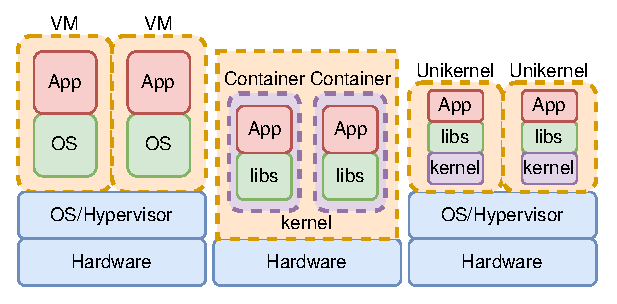
\includegraphics[width=\linewidth]{images/Figure5}
	\end{center}
	\vspace{-0.6cm}
	\caption{Architectural differences between VMs, containers and unikernels.}
	\label{fig:fig5}
\end{figure}
%
%
\section{Deployment}\label{sec:deployment}
%
Over the years different approaches evolved how to deploy infrastructure and applications. The difference just gets more amplified, when CC and microservices get into the picture, where frequent deployment is very common. 

Deployments in such complex environment can be separated by how they handle changes on existing infrastructure or applications on:

\begin{itemize}
	\item \textbf{A mutable model} is a model where we have in place changes which mean that the parts of the existing infrastructure or applications get updated or changed to do an update. In place change can produce some problems, and has:
	
	\begin{enumerate}[start=1,label={(\bfseries \arabic*)}]
		\item more risk because in-place change may not finish, which puts our infrastructure or the application in a possible bad state. This is especially a problem if we have a lot of services and multiple copies of the same service. The possibility that our system is not on is a lot higher.
		\item high complexity, this is a direct implication of the previous feature. Since our change might not get fully done, it cannot be guaranteed that our infrastructure or application is transitioned from one version to another -- change is not \textbf{discrete}, but \textbf{continues} since we might end up in some state in between where we are now and where we want to be.
	\end{enumerate}
	
	\item \textbf{An immutable model} is a model where no in-place changes on existing infrastructure or application are done whatsoever. In this model, the previous version is replaced completely with a new version that is updated or changed compared to the previous version. The previous version gets discarded in favor of the new version. Compared to the previous model, immutable deployment:
	
	\begin{enumerate}[start=1,label={(\bfseries \arabic*)}]
		\item has less risk, since the existing infrastructure or the application, is not changed, but a new one is started and the previous one is shut down. This is important especially in DS where everything can fail at any time.
		\item has less complexity of the mutable deployment model. This is a direct implication of the previous feature since the previous version is shut down and fully replaced with the new one. This is a \textbf{discrete} version change and atomic deployment with deferring deployments with fast rollback and recovery processes.
		\item requires more resources~\cite{Helland16}, since both versions must be present on the node for this process to be done. The second problem is the data that the application has generated should not be lost. The problem is solved by externalizing the data. We should not rely on local storage but store that data elsewhere, especially when the parts of the system are volatile and changed often. The key advantage of this approach is avoiding downtime experienced by the end-user when new features are released. 
	\end{enumerate}
\end{itemize}

Immutability is a simple concept to understand and simplifies a lot especially in DS~\cite{Helland16}. Write down some data, and ensure that it never changes. It can never be modified, updated, or deleted~\cite{perry2020art}. When this is combined with the promise that downtime can be avoided especially in complex DS, it is clear why the immutable model is gaining more and more popularity (especially with the arrival of containers). 

Immutable infrastructure deployment offers several benefits on how to deploy changes. Even in production, it is easier to switch to a whole new version. These strategies include:

\begin{itemize}
	\item \textbf{Blue-Green deployment}, this strategy requires two separate environments: \textbf{(1)} \textit{Blue} current running version, and \textbf{(2)} \textit{Green} is the new version that needs to be deployed. When there is satisfaction that the green version is working properly, the traffic can be gradually rerouted from the old environment to the new one,  for example by modifying the Domain Name System (DNS). This strategy offers near-zero downtime.
	\item \textbf{A canary update} is a strategy where a small subset of requests is directed to the new version --- the canary, and the rest of them are directed to an old version. If the change is satisfactory, the number of requests can be increased, and it should be monitored how the service is working with increasing load, if there are errors, etc.
	\item \textbf{Rolling update} strategy updates large environments, a few nodes at the time. The setup is similar to blue-green deployment, but here there is a single environment. With this strategy, the new version gradually replaces the old one. If for whatever reason the new version is not working properly on the larger number of nodes, rolling back to the previous version can always be done.
\end{itemize}

\noindent
With mutable infrastructure, these strategies would be hard to implement, and maybe it is not possible at all. Besides infrastructure deployment, there is another side that we must be considered, and that is how to describe these deployments. Two different strategies can be considered here:

\begin{itemize}\label{lab:dep_types}
	\item \textbf{Imperatively}, with this option users have to write code or specific instructions step by step what the specific tool needs to do so that the application or infrastructure is properly set up. In this approach, we have a \textit{smart} user who describes \textit{dumb} machine what is needed to be done and in what order to achieve the desired state.
	\item \textbf{Declaratively}, with this option a user has to describe the end state or what is his desired state, and the tool needs to figure out the way how to do this. Here we have a \textit{smart system} that will find a way how to achieve the \textbf{desired state}, and we have a user who\textit{does not care} in what order actions need to be done --- that is what the system needs to do. Users do not need to worry about timing, this simplifies the whole process and the code always represents the latest state. With this type of deployment, we can offer users, two different models:
	
	\begin{enumerate}[start=1,label={(\bfseries \arabic*)}]
		\item using existing platform independent formats that users are familiar with, like \textit{JSON, YAML, XML}, etc.
		\item using a domain-specific language (DSL) that users need to learn, but we might be able to optimize description.
	\end{enumerate}
\end{itemize}

\noindent
So far, the first option is preferred by many companies, because users are already familiar with these formats, and does not require developers time to develop new DSL. If the platform becomes too complicated then it makes sense to develop DSL for this purpose.

Figure~\ref{fig:fig12} summarizes the difference between mutable and immutable deployment models.

\begin{figure}[H]
	\begin{center}
		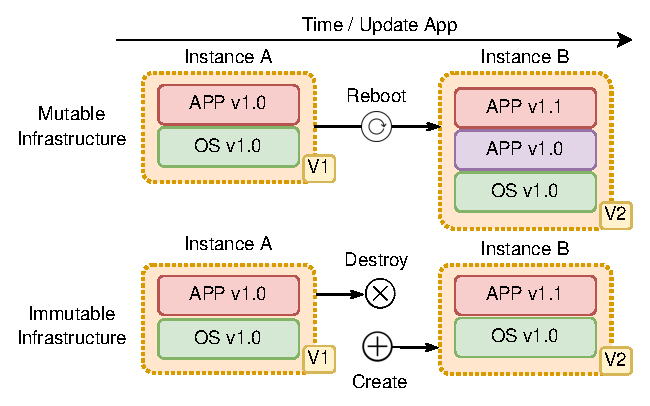
\includegraphics{images/Figure12}
	\end{center}
	\vspace{-0.6cm}
	\caption{Difference between mutable and immutable deployment models.}
	\label{fig:fig12}
\end{figure}

\noindent
With the introduction of \textit{LinuxKit}, Linux subsystems are based around very secure containers. With LinuxKit, every part of the Linux subsystem runs inside the container, so a Linux subsystem can be assembled with services that are needed. As a result, systems created with LinuxKit have a smaller attack surface~\cite{abs-1802-10375} than general-purpose systems. 

This is important not only from the security point of view but also for infrastructure deployment as well. Specific OSs can be created, based on the containers for a different purpose. They can be updated, changed, and adapted for every machine or purpose needed.

Deployment is based on changing parts of the OS, and services that run inside the containers. As a result, everything can be removed or replaced. It's highly portable and can work on desktops, servers, IoT, mainframes, bare metal, micro data centers at the edge, and virtualized systems.

\section{Infrastructure as software}~\label{sec:ias}
%
The infrastructure needs to be constantly deployed and maintained, so it would be beneficial to view the infrastructure as software (IaS)~\cite{Fitzgerald}. The benefit of this approach lies in the already available tools, principles, and techniques (e.g. reuse, testing, modeling, and evaluation) that can equally be used for the infrastructure definitions ~\cite{Osterweil, Fitzgerald}.

In his work~\cite{Osterweil}, Osterweil et al. argue that software and software processes share some similar characteristics: \textbf{(1)} both are executed, \textbf{(2)} both have requirements that need to be understood, \textbf{(3)} both benefit from being modeled, and \textbf{(4)} both can be guided by measurement.

Fitzgerald et al.~\cite{Fitzgerald} argue that process programming, defined by Osterweil~\cite{Osterweil} et al., is applicable in the infrastructure domain. The authors claim that it is useful to extend the “software process as software” paradigm to include infrastructure as software (IaS). The move towards multi-tier systems that involve cloud and cyber-physical systems will only stimulate the connection between software and reliable infrastructure systems.

Looking at the infrastructure configuration as the software allows application developers to venture into the “infrastructure programming”~\cite{Fitzgerald}, allowing platforms and infrastructure to be managed in a similar way as the software is.

In a cloud environment, it is an essential technique to properly implement continuous deployment, giving us tools to automate the configuration and provisioning process of infrastructure using cloud instances~\cite{RahmanMW19}. Wittig et al. describe it as a process of managing and provisioning computer data centers through machine-readable definition files, rather than physical hardware configuration or interactive configuration tools~\cite{wittig2018amazon}. 
%
%
\subsection{Infrastructure as code}
%
In modern cloud and microservices era, a new strategy to manage and deploy complicated infrastructure elements -- Infrastructure as code (IaC). In his book~\cite{wittig2018amazon} Wittig et al. describe it as a process of managing and provisioning computer data centers through machine-readable definition files, rather than physical hardware configuration or interactive configuration tools. 

IaC has grown in popularity in recent years because it applies the same kind of version control and repeatability to the orchestration of the infrastructure as developers use for applications source code~\cite{ArtacBNGT17}. The second benefit is that configuration is decoupled from the system, it can more readily be deployed on a similar system elsewhere. 

IaC is a continuation of earlier works of Osterweil et al.~\cite{Osterweil}, and Fitzgerald et al.~\cite{Fitzgerald}, trying to move infrastructure to level of software, keeping existing tools, best practices and techniques. It relys on the \textbf{reconciler pattern}~\cite{luksa2018kubernetes}, widely used in scheduling systems like Kubernetes.

This pattern enables tracking of resources using two simple states: \textbf{(1)} expected state, and \textbf{(2)} current state. The expected state represents the desired state, while the current state refers to the actual system state. The reconciler pattern runs a \textbf{reconciliation loop} that ensures that the current state remains the same as the expected state.

Every node must provide its current state regularly, and when some state is divergent from the desired state, the system must act to ensure that this situation is corrected automatically. The node can send its state over existing channels e.g., \textbf{health-check} pings to minimize load and data transferred over the network, or a dedicated channel just for this purpose may exist.
%
%
\section{Development roles}\label{sec:dev_roles}
%
In our modern internet-connected world of applications, we have several distinctive development roles. Each of them plays an important role so that modern software runs smoothly, and with less downtime. These development roles could be separated into a few categories (focus is on the technical roles):

\begin{itemize}
	\item \textbf{A developer} is usually a person responsible for developing software for the user. A developer is responsible for maintaining existing, and/or developing new features. There could be different sub-roles, dealing with specific parts of the complex software systems.
	\item \textbf{DevOps} role represents a multidisciplinary organizational effort to automate application deployments through continuous delivery of new software updates~\cite{LeiteRKMM20}. It combines software development with technology operations~\cite{JabbariAPT16} to shorten the development life cycle.
	\item \textbf{Site Reliability Engineer (SRE)} role is responsible for availability, latency, performance, efficiency, change management, monitoring, emergency response, and capacity planning~\cite{beyer2016site}. It is a software engineering role and needs to have an understanding of the fundamentals of computing~\cite{JonesUN15}, applied to the infrastructure and operations problems.
\end{itemize}

\noindent
DevOps and SREs seem to be similar roles, they are both trying to bridge the gap between development and operations. As such they have a very large conceptual overlap in how they operate~\cite{46939}, but also have some differences. 

Table~\ref{tab:table10} sums the differences between the DevOps and SREs.

\begin{table}[H]
	\begin{center}
		\begin{tabular}{l|l|l}
			\textbf{Feature} & \textbf{DevOps} & \textbf{SREs}\\
			\hline
			\textbf{Task} & \multirow{2}{10em}{Scaling, uptime, robustness} & \multirow{2}{10em}{Development pipeline} \\
			& & \\
			\textbf{Essence} & Practices and metrics &  Mindset and culture \\
			\textbf{Team structure} & \multirow{3}{10em}{Wide range of roles: QA, developers, SREs etc.} &  \multirow{3}{10em}{SREs with operations and development skills} \\
			&  &  \\
			&  &  \\
			\textbf{Focus} & \multirow{2}{10em}{Development and delivery continuity} & \multirow{2}{10em}{System availability and reliability} \\
			&  &  \\
			\hline
			\textbf{Goal} & \multicolumn{2}{c}{\multirow{2}{15em}{Bridge the gap between development and operation}} \\
			&  &  \\
		\end{tabular}
	\end{center}
	\vspace{-0.5cm}
	\caption{Differences between DevOps and SREs.}
	\label{tab:table10}
\end{table}

\noindent
In modern complex software development, SREs should keep things running smoothly, while DevOps principles should be used to improve processes. 

So it is not either/or, but it seems that a combination of approaches may provide the best results. However, in some smaller organizations, these roles can overlap.
%
%
\section{Concurrency and parallelism}\label{sec:concurency_parallelism}
%
People usually confuse these two concepts. Even though look similar, they are a different way of doing things. In his speech, Rob Pike~\cite{Pike} gives a great explanation and examples on this topic. He also gives great definitions of these concepts like:

\begin{itemize}
	\item \textbf{Concurrency} is composition of independently executing things. Concurrency is about dealing with a lot of things at once.
	\item \textbf{Parallelism} is the simultaneous execution of multiple things. Parallelism is about doing a lot of things at once. 
\end{itemize}

\noindent
These things are important, especially when building applications and systems that should achieve very high throughput. They must be built with a good structure and a good concurrence model. These features enable possible parallelism, but with communication~\cite{Pike}. These ideas are based on Tony Hoare work of Communicating Sequential Processes (CSP)~\cite{Hoare78}.

\subsection{Actor model}\label{sec:actor_model}
%
An actor model, the main idea is based around \textbf{actors} which are small concurrent code, that communicate independently by sending messages, removing the need for lock-based synchronization~\cite{Hewitt}. This model proposes a similar idea to Tony Hoare's in his work with CSP~\cite{Hoare78}, and actors are often confused with CSP. 

Table~\ref{tab:table6} gives differences between an actor model and CSP.

\begin{table}[h!]
	\begin{center}
		\begin{tabular}{l|l|l}
			\textbf{Feature} & \textbf{CSP} & \textbf{Actor model}\\
			\hline
			\textbf{Fault tolerance} & Distributed Queue &  Supervisors hierarchy \\
			\textbf{Process identity} & Anonymus & Concrete \\
			\textbf{Composition} & NA & Applicable \\
			\textbf{Communication} & Queue & Direct \\
			\textbf{Message passing} & Sync & Async\\
		\end{tabular}
	\end{center}
	\vspace{-0.5cm}
	\caption{Differences between actor model and CSP.}
	\label{tab:table6}
\end{table}

\noindent
Actors do not share a memory, and they are isolated by nature. An actor can create another actor/s and even watch on them in case they stop unexpectedly. When an actor finished its job, and it is not needed anymore, it disappears. These actors can create complicated networks that are easy to understand, model, and reason about, and everything is based on a simple message passing mechanism. 

Every actor has a designated message box. When a message arrives, the actor will test the message type and do the job according to the message type he received. In this way, we are not dependent on lock-based synchronization that can be hard to understand, and it can cause serious problems.

The actor model is fault-tolerant by design. It supports crush to happen because there is a \say{self-heal} mechanism that will monitor actor/s, and when the crash happens it will try to apply some strategy, in most cases just restart actor, but other strategies could be applied. This philosophy is useful because it is hard to think about every single failure option.
%
%
%!TEX root =  main.tex
\chapter{Research review}\label{chapter:Review}
%
Faced real issues and limits of cloud computing, both academia, and the industry started researching and developing viable solutions. Some research is focused more on adapting existing solutions to fit EC, while others experiment with new ideas and solutions. 

In this Chapter, we present the results of our research reviews addressing issues discussed earlier. in Section~\ref{sec:nodes_organization} we review existing nodes organizational abilities, as well platform models from industry and academia in Section~\ref{sec:nodes_organization}. In Section~\ref{sec:task_offloading} we review cloud offloading techniques. In Section~\ref{sec:applications} we review some applicartio models, and we give position of this thesis compared to all revied aspects in Section~\ref{thesis_position}.
%
%
\section{Nodes organization}\label{sec:nodes_organization}
A zone-based organization for edge servers (ES) presented by Guo et al. in~\cite{GuoRG20}, gives an interesting perspective on EC in a smart vehicles application. They showed how zone-based models enable continuity of dynamic services, and reduce the connection handovers. Also, they show how to enlarge the coverage of ESs to a bigger zone, thus expanding the computing power and storage capacity of ESs. Since one of the premises of EC is geo-distributed workloads, organizing ESs into zones and regions could potentially benefit EC. 

Baktir et al.~\cite{BaktirOE17} explored the programming capabilities of software-defined networks (SDN). Findings show SDN can simplify the management of the network in cloud-like environment. SDN is a good candidate for networking because it hides the complexity of the heterogeneous environment from the end-users.

Kurniawan et al.~\cite{inbookKurniawan} argue about very bad scalability in centralized delivery models like cloud content delivery networks (CDN). They proposed a decentralized solution using nano DCs as a network of gateways for internet services at home~\cite{inbookKurniawan}. These DCs are equipped with some storage as well. Authors show a possible usage of nano DCs for some large scale applications with much less energy consumption. 

Ciobanu et al.~\cite{CiobanuNPDMM19} introduce an interesting idea called drop computing. The authors show that we can compose EC platforms ad-hoc, thus enabling collaborative computing dynamically, using a decentralized model over multilayered social crowd networks. Instead of sending requests to the cloud, drop computing employees the mobile crowd formed of nearby devices, hence enabling quick and efficient access to resources. The authors show an interesting idea of how to form a computing group ad-hoc. Forming ad-hoc platforms from crowd resources might raise a few possible concerns: $(1)$ crowd nodes availability, and $(2)$ offered resources. Crowd nodes might be an interesting idea as a backup option, in cases we need more computing power or storage and there are no more available resources to use.

MDCs are an interesting model and area of rapid innovation and development. Greenberg et al.~\cite{GreenbergHMP09} introduce MDCs as DCs that operate in proximity to a big population (on contrary to nano DCs that serves a lot smaller population), thus minimizing the latency and costs for end-users~\cite{ShiHPANZ14, GreenbergHMP09}, 
%, WangZXYH19}
and reducing the fixed costs of traditional DCs. Minimum size of an MDCs is defined by the needs of the local population~\cite{GreenbergHMP09, AbbasZTS18}, with agility as a key feature. Here agility means an ability to dynamically grow and shrink resources and satisfy the demands and usage of resources from the most optimal location~\cite{GreenbergHMP09}.
%
%
\section{Platform models}\label{sec:platform_models}
%
Kubernetes~\cite{BurnsGOBW16} is an open-source variant of Google orchestrator Borg \cite{VermaPKOTW15}.  All workloads end in the domain of one cluster~\cite{BurnsGOBW16, VermaPKOTW15, RossiCPN20}. Rossi et al.~\cite{RossiCPN20} focuses on adapting Kubernetes for geo-distributed workloads using a reinforcement learning (RL) solution, to learn a suitable scaling policy from experience. Like every other machine learning implementation this could be potentially slow due to the required model training. Kubernetes is a promising solution, but it might not be the best proposal for EC. By design, Kubernetes operate in a completely different environment from EC. The second potential issue is the deployment concept that might be too complicated for EC workloads. On the other hand, there are a few ideas that are worth exploring, such as loosely coupling elements with labels and selectors. Nonetheless, researches show that adapted Kubernetes architecture works for geo-distributed workloads like EC.

Ryden et al.~\cite{RydenOCW14} present a platform for distributed computing with attention to user-based applications. Unlike other systems, the goal is not to implement a resource management policy, but to give users more flexibility for application development. Users implement applications using Javascript (JS) programming language, with some embedded native code for efficiency. Similar to~\cite{CiobanuNPDMM19}, the authors use volunteer nodes to run all the workloads, with the difference that some nodes are used for storage, while others are used for calculation. Sandboxing technique protects nodes running applications from malicious code. It is an interesting idea to show how users can develop their applications and run them in an EC environment.

L{\`{e}}bre et al.~\cite{LebrePSD17} describe a promising solution of extending OpenStack, an open-source IaaS platform for fog/edge use cases. They try to manage both cloud and edge resources using a NoSQL database. Implementation of a massively distributed multi-site IaaS, using OpenStack is a challenging task~\cite{LebrePSD17}. Communication between nodes of different sites can be subject to important network latencies~\cite{LebrePSD17}. The major advantage is that users of the IaaS solution can continue using the same familiar infrastructure. In~\cite{ShaoLFJL19} Shao et al. present a possible MDCs structure serving only the local population, in the smart city use-case.

In~\cite{NingLSY20}, the Ning et al. show current open issues of EC platforms based on the literature survey. They illustrate the usage of edge computing platforms to build specific applications. In the survey, the authors outline how CC needs EC nodes to pre-process data, while EC needs massive storage and strong computing capacity of CC.

In~\cite{abs-1802-10375} the de Guzm{\'{a}}n et al. present solution based on Kubernetes that use Kubernetes Deployment Manifests in order to reuse successful principles from Kubernetes by creating  virtual machine for each Pod using Linuxkit. Their solution is based on the immutable infrastructure pattern, and instead of containers they use the virtual machines as the unit of deployment. Authors prove that the attack surface of their system is reduced since Linuxkit only installs the minimum OS dependencies to run containers. It represent interesting usage of LinuxKit to deploy OS dependencies, and immutable infrastructure pattern, but VMs might be a bit problem for small devices, and ARM nodes as well as complex flow of Kubernetes application model. But nonetheless, it is interesting extension of Kuibernetes framework and prove that LinuxKit can be used for immutable infrastructures with custom OS.

In~\cite{SamiM20} Sami et al. show interesting platform for dynamic sevices distribtion over Fog nodes using volunteer nodes. Their platform is tuned for container placement with relevance and efficiency on volunteering fog devices, near users with maximum time availability and shortest distance. They do this \textit{on the fly}  with improved QoS.

There are few industry operating frameworks for EC, like Amazon Greengrass~\cite{kurniawan_2018}, deeply connected to the entire Amazon cloud ecosystem, or KubeEdge~\cite{KubeEdge}, a lightweight extension of Kubernetes framework. These frameworks are mainly used for user-based applications, while, for instance, General Electric Predix~\cite{GE_Predix} is a scalable platform used for industrial IoT applications.
%
%
\section{Task offloading}\label{sec:task_offloading}
%
As already mention in~\ref{sec:mobile_computing} EC nodes rely on the concept of data and computation offloading from the cloud closer to the ground \cite{KhuneP19}, while heavy computation remains in the cloud because of resource availability~\cite{NingLSY20}. 

Offloading is effective when using cloud servers but this principle introduce long latency, which some applications can't tolerate. On the other hand mobile devices and sensors do not have sufficient battery energy for task offloading~\cite{MaoZL16}. The computation performance may be compromised due to insufficient battery energy for task offloading, so these devices might send their data to nearby EC nodes.

In literature, there are few platforms proposing task offloading~\cite{ShiHPANZ14, KhuneP19, ChenHLLW15, LinLJL19, JiangCGZW19, MaoZL16} to the nearby edge layer. These offloading techniques are based on different parameters, options, and techniques to put tasks to different sets of nodes in such a way that it won't drain mobile devices and sensors baterry. After compuitation is done, this edge layer send pre-processed data to the cloud for further analyse, storage et.

In~\cite{SamiM20} authors used Evolutionary Memetic Algorithm (MA) to solve their multi-objective container placement optimization problem to achieve better QoS.
%
%
\section{Application models}\label{sec:applications}
%
Ryden et al.~\cite{RydenOCW14} present Nebula, a platform for distributed computing. Users develop their applications using JS only. This restriction comes from using Google Chrome Web browser-based Native Client (NaCl) sandbox~\cite{YeeSDCMOONF10}. JS is a popular language at the moment, but the restriction of a single language might be a deal-breaker for some usages. If standard virtual machines become too resource-demanding, a solution using containers could provide sandboxing and bring better resource utilization.

In~\cite{SatyanarayananBCD09} Satyanarayanan et al. represent an interesting view on cloudlets s a \say{data center in a box.}. They give example that cloudleta should support the wide range of users, with minimal constraints on their software. They pun emphesis on transient VM technology. The emphasis on transient VMs is beacuse cloudlet infrastructure is restored to its pristine software state after each use, without manual intervention. In the time they conduct they reserach containers might not be working solution or it might be hard to use them. By today standards, containers may even fit better, and pack more user softvare on same hardware. This may be case for the unikernels, once they reach wider adoption rate and stable products.

Various Kubernetes variants lik~\cite{KubeEdge, RossiCPN20}, give users possibiliety to run different applications like web servers and databses even on smaler devices cretaing green DC~\cite{ArocaG12}.

Satyanarayanan et al.~\cite{SatyanarayananK19} propse concept of edge-native applications that will separate space into 3 tiers.Tier 1 represent various mobile and IoT devices. These devices produce a lot of data. Tier 2 represent applications running in cloudlets or other EC models, that will pre-process, fiter data before it goes further. Finaly, tier 3 represnet classic cloud applications that will accept pre-processed and filer data from previous tier. This represent interesting concept, and give wide space for users and application developement.

In~\cite{inproceedingsBeck} Beck et al. argue that applications should use message bus, because most mobile edge applications are expected to be event driven.  Message bus system is an interesting, because virtualized applicatoin can subscribe to message streams, i.e., topics. And if for some reason mobile edge applications can't reach close EC server, it can always send data to cloud. So cloud applications should be changed so so slightly, just to accept this case.
%
%
\section{Thesis position}\label{sec:thesis_position}
Different from the aforementioned work,this thesis focuses on descriptive dynamic organization of geo-distributed nodes over an arbitrary vast area that lacks in other solutions. To achieve such a task, thesis model is influenced by the CC organization, but adapted for a different environment such as EC. These adaptations are followed by clear Separation of concerns (SoC) and EC applications model. All these allow us to push the whole solution more towards EC as a service model like any other utility in the cloud.
%
%
%!TEX root =  main.tex
\chapter{Micro clouds}\label{chapter:Micro_clouds}
%
In this section, the core idea of this thesis will be presented, from the point of view how such a model can be formed and described, and what is important so that such a system operates properly. A \textbf{micro-cloud} model will be described, based on the CC organizational model.  The presented model will be able to support EC as a service, amongst other applications and use-cases. 

Throughout this section, we are going to rely on the research presented in chapters~\ref{chapter:Intro} and~\ref{chapter:Review}, and make a connection with the existing CC model.

In Section~\ref{sec:configurable_model_structure} we present a high overview of the system -- an architecture that is influenced by the standard CC model but adapted for a different environment. Section~\ref{sec:separation_of_concerns}introduces the separation of concerns model for previously defined system architecture. Section~\ref{sec:application_model} presents a possible application model and how users can utilize newly created architecture fully. Application models are based on existing development models, so that transition is fairly easy. How this system could be offered as a service, and which options can be offered to the potential users for developing their applications is discussed in Section~\ref{sec:as_a_service_model}. Section~\ref{sec:immutable_infrastructure} presents the desired option for infrastructure and application deployment, and why immutability is important in a micro-cloud geo-distributed environment. Section~\ref{sec:formal_model} presents why formal models are important in computer science and DS in particular, as well as formal models of all protocols used in system formation and operation.  Section~\ref{sec:long_live_transactions} shows transactions that appear in such complex system, and garbage collection done on resources that are not used anymore. Section~\ref{sec:system_observability} shows system observability mechanisms important for geo-distributed environments like micro-clouds. Section~\ref{sec:access_pattern} shows access patterns that could be used in micro-clouds and geo-distributed environments. Section~\ref{sec:repercussion} gives repercussion of the proposed model, and how it can be used as a stand-alone model where other features could be implemented on top of that or used as service for other, existing, systems. This chapter is concluded with Section~\ref{sec:limitations}, which presents limitations of our model.
%
%
\section{Configurable Model Structure}\label{sec:configurable_model_structure}
%
In his work~\cite{SatyanarayananK19} Satyanarayanan et al. propose a new architecture pattern and separation into the three tiers, where every tier or layer has a distinct role. This idea is a very powerful one because applications can now be split into parts and optimized for the specific role in the global picture. On the other hand, too many moving parts mean more problems, and the whole system is potentially more prone to errors and failures.

If the previous model is taken and combined with MDCs and a zonally based server organization, a good starting point for building micro-cloud infrastructure, and EC as a service is achieved. This extension is an interesting move because the computing power and storage capacity that serves the nearby population can then be extended. This base model is just a starting point that is promising, but to make a fully functional model, it needs to be made more available and resilient with less latency. To achieve such behavior, these concepts have to be extended and adapted for different usage scenarios, but a geo-distributed idea from our vision should not be lost.

To extend the system in a new direction, we can look for some inspiration in existing systems that are proven and working. This is especially important in DS, so we want to lower down the complexity and avoid known problems by sticking to existing models and algorithms. When the CC design is observed, it can be seen that every single part in that system contributes to a more resilient and scalable system. On the high level, the CC architecture is separated into few building blocks that make the whole system lot easier to understand, maintain and operate.

The first building block of CC architecture is a cluster, and a cluster can be defined as a set of nodes or servers that operate as a single unit to achieve some goal. This is where resources are, and this is where user applications are running on. The next building block that consists of multiple clusters is called Regions (or DCs). Regions are isolated and independent from each other, and they contain resource application needs. These resources come in form of clusters. Regions are usually composed of a few availability zones~\cite{SouzaMFAK19}. These zones are the defense against the fail. If for whatever reason, one zone fails or goes offline, there are still more of them to serve user requests, there is a better availability, scalability, and resilience.

If we now observer micro-clouds as geo-distributed systems, we can use a similar model, with some adaptations. Rely on a similar proven strategy, do not reinvent the wheel, but adopt for the different use-case.

Table~\ref{tab:table5} presents similar concepts between CC and edge-centric computing (ECC) concepts. The accent is here put on the difference between the physical logical concepts in the two models.

\begin{table}[h!]
	\begin{center}
		\begin{tabular}{l|l}
			\textbf{Edge centric computing} & \textbf{Cloud computing}\\
			\hline
			Topology (logical) & Cloud provider (logical)\\
			Region (logical) & Region (physical)\\
			Cluster (physical) & Zone (physical)\\
		\end{tabular}
	\end{center}
	\vspace{-0.5cm}
	\caption{Similar concepts between cloud computing and ECC.}
	\label{tab:table5}
\end{table}

\noindent
Since we are talking about geo-distributed systems, our scenario is a little bit different than the one used in the standard CC model. We can still combine multiple EC nodes into clusters, that is what MDCs already propose. If we want to go a little bit further, we can define cluster as a:

\begin{definition}
	A micro-cloud cluster is a group of nodes that are virtually and/or geographically separated, that works together to provide the same service to clients.
\end{definition}

\noindent
Multiple node clusters could be combined into the next bigger logical concept of $region$. A region will increase the availability and reliability of both the system and applications. 

But the region in CC and ECC is not fully the same thing. In the standard CC model, the region is a physical thing or element of the existing infrastructure~\cite{SouzaMFAK19}, while in the ECC a region could be viewed differently, not as a physical element but rather as a logical element.A formal definition of a $region$ in ECC can now be given as:

\begin{definition}
	In a geo-distributed environment like ECC and micro-clouds, a concept of region is used to describe a set of clusters (that could be) scattered over an arbitrary geographic region. Regions are fully capable to accept or release clusters in the same way that clusters can accept or release nodes.
\end{definition}

\noindent
In MDCs, a cluster is as big as the population nearby that is using it~\cite{GreenbergHMP09}. If this is combined with the previous definition, then the minimum size of an ECC region can formally be defined as:

\begin{definition}
	Geo-distributed regions are composed of at least one cluster but can be composed of much more to achieve a more resilient, scalable, and available system.
\end{definition}

\noindent
With the previous definition, we have to be careful not to introduce huge latency in the system. To lower the region latency, the vast distances between clusters should be strongly avoided in normal circumstances. new nodes have to be brought and connected physically to the rest of the infrastructure~\cite{Hamilton07}, while in the ECC the region should be extended just by changing the definition to whom the specific cluster belongs.

Multiple regions should be able to form a second logical layer -- $topology$. In the geo-distributed systems such as ECC or micro-clouds, topology can formally be described as:

\begin{definition}
In geo-distributed systems, topology represents the highest logical concept that is composed of a minimum of one region and could span over multiple regions. Topology is fully capable to accept new or release the existing regions. 
\end{definition}

\noindent
With these simple abstractions, any geographical region can be easily covered with the ability to shrink or expand clusters, regions, and topologies. Size and formation of $clusters$, $regions$, and $topologies$ should be a matter of need, agreement, and usages of nearby population similar to the size of MDCs~\cite{GreenbergHMP09}, and modeling in Big Data systems~\cite{SonbolOAA20, WangCAL14}. This separation and organization gives one interesting feature. A more natural administrative division of some region can be followed, and resources can be organized by population usages.

The organization of these concepts should be fully optional. So for example, we could fit clusters in an interval of nano-DCs~\cite{inbookKurniawan} and MDCs~\cite{GreenbergHMP09} or as wide as the whole city or as small as all devices in a single household and everything in between. Formally, the size of some cluster $c$ can be represented like:

\begin{equation}
	c \in \left[ nano\ DCs,\ MDCs \right]
\end{equation}
\myequations{Cluster size limits}

\noindent
If we go a little bit further, we can represent the city as one region, where parts of the city are organized into clusters. A city topology can even be formed by splitting the city into multiple regions containing multiple clusters, and ultimately a country topology can be formed by splitting the country into regions, with cities being clusters.\\ 

Nodes that belong to the same cluster should run some form of membership protocol presented in~\ref{sec:memership_protocol}. Gossip style protocols, like SWIM~\cite{DasGM02} (cf. page~\pageref{swim}), are standard in the cloud environment. The same strategy could be applied here, used in conjunction with replication mechanisms~\cite{LiBCL20, CauCBFCEB16, CRDTS_Nuno} making the whole system more resilient. 

Replication could be used not only in nodes inside the cluster, but data can also be replicated in clusters inside the region and even in regions inside topology. This property should exist, but it should be controlled by users depending on how resilient and available the system he/she wants and needs. In~\cite{inproceedingsSimic2} Simi\' c et al. take a look from a theoretical point of view on CRDTs usage, to achieve SEC in EC. The authors conclude that CRDTs could be a natural fit to EC as long as we are aware of the potential pitfalls of CRDTs.

Single $topology$ reflects one CC provider, so multiple topologies are forming micro-clouds that can help CC with huge latency issues, pre-processing in huge volumes of data, and relax and decentralize strict centralized CC model.

These micro-clouds have much fewer resources compared to standard clouds, but they are much closer to the user meaning they have a much faster response. In the case of storage, if data is not present at the time of user request, they can pull data from the cloud and cache it for later. Formaly, the position of micro-clouds $mc$ in between CC and EC like:

\begin{equation}
mc \in \left( Cloud\ computing,\ Edge\ computing \right)
\end{equation}
\myequations{Position od micro clouds.}

\noindent
Exclusiveness in the previous formula, means that position of micro-clouds is moveable in between CC and EC depending do we want our model to be more CC like or more EC like, but it should not become one of them. It could be integral part for both of these models (even at the same time).

Three-tier~\label{lab:three-tier} architecture with numerous clients at the bottom, micro clouds in the middle, and cloud on the top, seem to resemble cache level architecture in CPU~\cite{FarshinRMK19}. 

On lower levels, response time is the fastest, since data is processed closer to the source. At the same time, there is a limited storage capacity and processing power. As we go on the upper tiers, there is more and more storage capacity and processing power, but the response time is higher and higher, especially when distance and huge volumes of data that need to be moved to the cloud are considered.

Figure~\ref{fig:fig9}. shows the three-tier architecture, with the response time and resource availability.

\begin{figure}[H]
	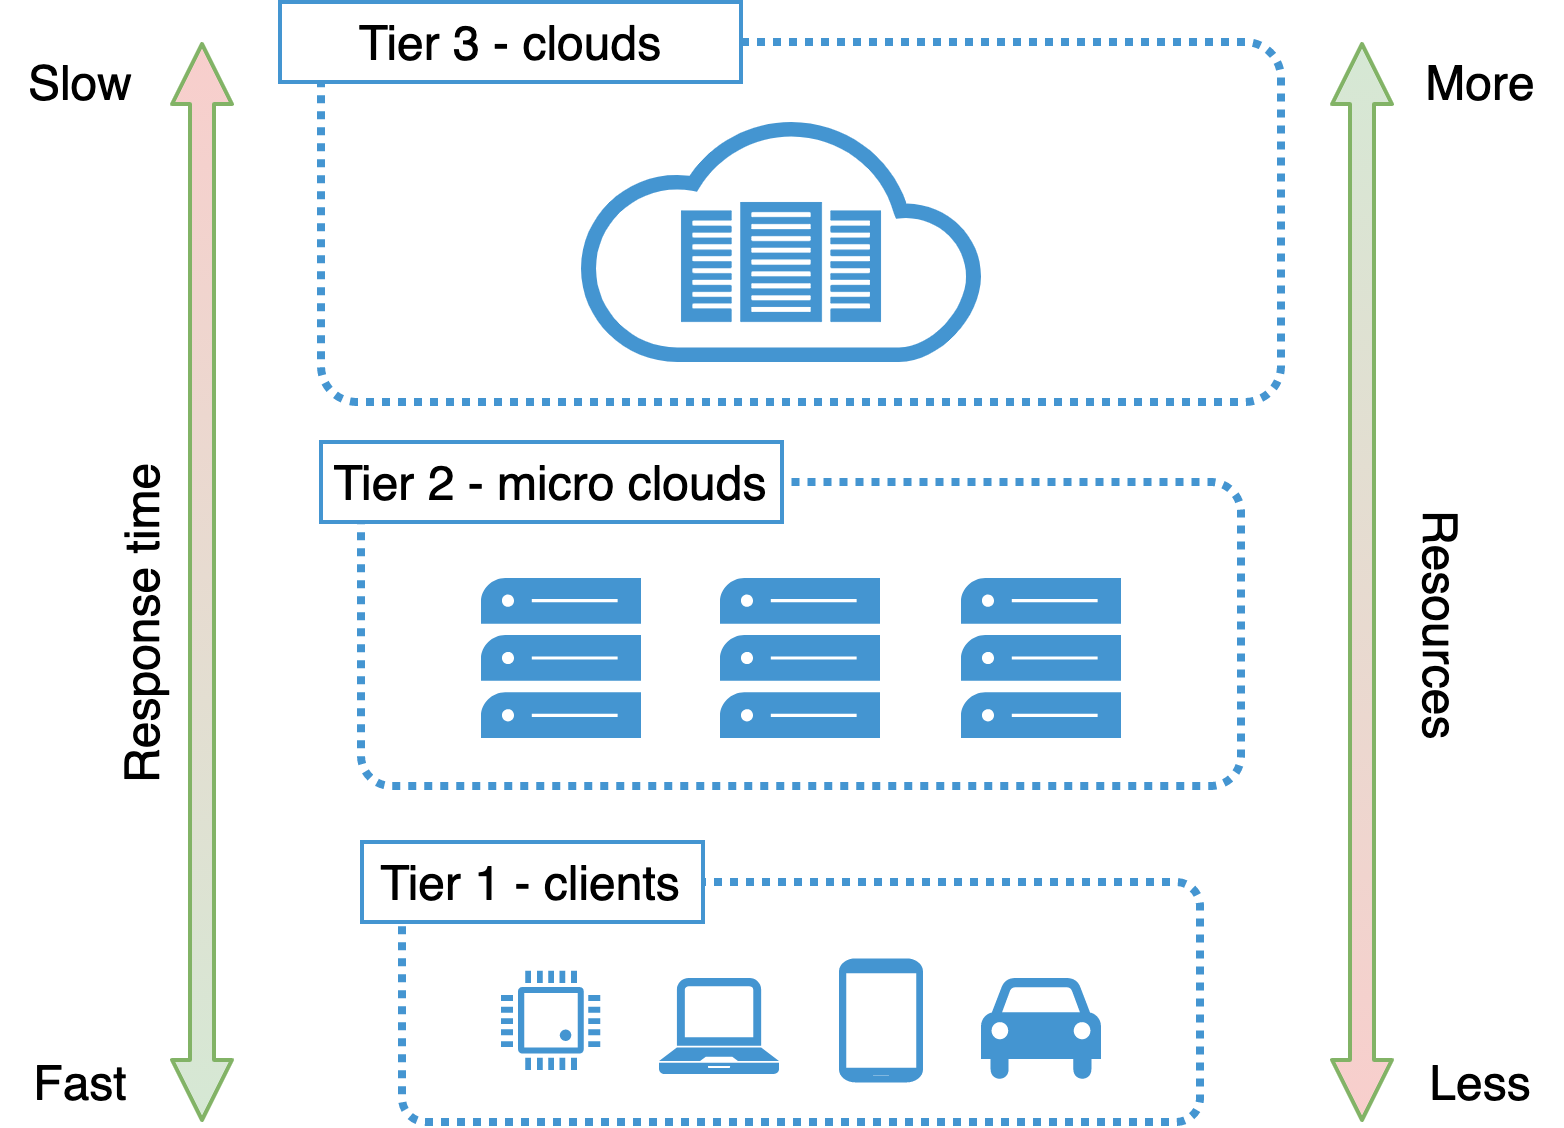
\includegraphics[width=\linewidth]{images/Figure9}
	\vspace{-0.7cm}
	\caption{Three tier architecture, with the response time and resource availability}
	\label{fig:fig9}
\end{figure}

\noindent
In everything as a service model~\cite{DuanFZSNH15}, ECC as a service fits in between CaaS and PaaS, depending on the user needs. 
%
%
\section{Separation of concers}\label{sec:separation_of_concerns}
%
In his work, Jin et al.~\cite{JinCJL14} introduces three core concepts to fully describe physical services, and specifies their relationships. Concepts that authors propose are: \textbf{(1)} Devices, \textbf{(2)} Resources, and \textbf{(3)} Services. This separation is interesting because we can rely on it in a geo-distributed environment, to describe SoC for micro-clouds.

One of the most important part of every system, is the SoC model. This is especially important if a platform to be offered as a service is going to be created. With some adaptations, our SoC model can be based on concepts proposed by Jin et al.~\cite{JinCJL14} in three layers, as depicted in Figure~\ref{fig:fig10}. 

The layer on the very bottom of the three-tier architecture (cf.~Figure~\ref{fig:fig10}) consists of various devices. These devices are important because they represent main \textit{data creators} but at the same time, they are main \textit{services consumers}. 

The layer in the middle (cf.~Figure~\ref{fig:fig10}) represents resources or EC nodes. These resources have a very important spatial feature, and as such, they indicate the range of their hosting devices~\cite{JinCJL14}. This means that the developers at any given time must know the topology of the system, the resource spread, and utilization across clusters. Besides that main information, users must know the state and health of every application.~\label{soc:resources}. If some EC node desires to be a part of the system, a node must obey four simple rules:

\begin{enumerate}[start=1,label={(\bfseries \arabic*)}]
\item a node must run an operating system with a usable file system;
\item a node must be able to run some isolation engine for applications, for example, containers or unikernels;
\item a node must have available resources for utilization so that applications can be run or data stored;
\item a node must have a stable internet connection;
\end{enumerate}

\noindent
One thing that is important to notice, is that all nodes in clusters, regions, and topologies are \textbf{equal} and there are \textbf{no special nodes}. Every node that joins the system must be able to store and process information.

Last but certainly not least layer represents services. These services expose resources through some interface and make them available over the internet~\cite{JinCJL14}. These services respond to the client requests immediately, if possible, or cache information~\cite{SatyanarayananBCD09,YaoXWYZP20} for future use. Unlike the previous two layers, services have one specific feature and span over two tiers of the system (cf.~Figure~\ref{fig:fig10}):

\begin{enumerate}[start=1,label={(\bfseries \roman*)}]\label{services}
	\item Services that exist in the micro-cloud, and they are responsible for filtering and data pre-processing before sending it to the cloud. Or cache information that was not available on a previous user request for some future use.
	\item Services in the standard cloud that should be able to accept pre-processed data, and they are responsible for computation and storage that is beyond the capabilities of ECC nodes. Services in the cloud should be able to take direct requests from the clients in a case when something catastrophic happens to the micro-cloud that is close to the user, and it is not able anymore to accept user requests.
\end{enumerate}

\noindent
This kind of services separation creates new application model that we present in detal in the secion~\ref{sec:application_model}. 

Figure~\ref{fig:fig10}. shows the proposed SoC for every layer of the ECC as a service model.

\begin{figure}[H]
	\includegraphics[width=\linewidth]{images/FIG1}
	\vspace{-0.7cm}
	\caption{ECC as a service architecture with separation of concerns.}
	\label{fig:fig10}
\end{figure}
%
%
\section{Applications Model}\label{sec:application_model}
%
Modern-day applications that should run in the cloud are advised to follow the cloud-native model~\cite{GannonBS17}. With this approach, we get applications that are easier to scale, more available, and less error-prone when compared to traditional web applications~\cite{GannonBS17}. 

Satyanarayanan et al. present the edge-native applications model~\cite{SatyanarayananK19} that should use the full potential of EC infrastructure, and keep good features of their cloud counterparts. 

When we introduced SoC for the micro-cloud model (cf. page~\pageref{services}), we described services that have one specific feature, and that is that these services span over two tiers of the system. This information is crucial for application development because we want to use the full potential of formed infrastructure, and keep good features of their cloud counterparts.

To satisfy the previously defined SoC model (cf. page~\pageref{services}), existing applications can be split into the \textbf{front} and \textbf{back} processing services. The front processing service is an edge-native application running inside some previously formed cluster to minimize latency, while the back service runs in the traditional cloud as a cloud-native application to leverage greater resources.

The front processing service will handle user requests coming to the nearby cluster, and communicate with the back processing services when needed to synchronize the pieces of information, cache data, or pass filtered or pre-processed data. Separation like that gives developers better flexibility and large design space when creating and optimizing their workloads.

With this model, we venture even deeper into understanding and applying the concept of \textbf{data locality} (cf. page~\pageref{ds:data_locality}). Since we have front and back processing services, we are committed to doing processing data closer to their source, instead of moving data to the cloud. This reduces latency and saves some users money on storing and processing unnecessary data.
%
%
\subsection{Execution models}\label{sec:execution_models}
%
Frontend services model should be packed in some standard way~\ref{sec:virtualization_techniques} and deployed in the wild, as an event-driven application, with the subscription policy to message streams, or infinite sequences~\cite{Rutten03} using topics~\cite{inproceedingsBeck}. The processing strategy is in the developer's hands, depending on the nature of the use-case. 

If a service is subscribed to some stream using a topic, for example, it is natural that events appear in their stream. There are two strategies for building a large-scale time-ordered event system:

\begin{enumerate}[start=1,label={(\bfseries \arabic*)}]
	\item \textbf{Fan out on write}, with this strategy, every service has some form of inbox, and when an event appears for some topic, that data is copied to every service that is subscribed to that topic. With these options, reads are fast, but writes are not. The more subscribers to the topic, the longer it takes to persist all updates. 
	\item \textbf{Fan in on read}, with this strategy, every topic has a sort of outbox where it can store data. When services read their streams, the system will read the recent data from the outboxes. Writes are fast, and used storage is minimal, but reads are difficult because to do this properly on a request-response deadline is not a trivial task to do.
\end{enumerate}

\noindent 
To implement those ideas without complicated synchronization, CRDTs could be used~\ref{crdts}. Companies like Soundcloud and Bet365 are already using them for the same or similar tasks.

Some examples of applications may include:

\begin{enumerate}[start=1,label={(\bfseries \arabic*)}]
	\item \textbf{events} that notify users if some value is above or below some defined threshold; 
	\item \textbf{stream} or processing data as it comes to the system;
	\item \textbf{batch} does processing in predefined times over some bigger collection of data ;
	\item \textbf{daemons} or processing that are that do some tasks or executions in the background without explicit user intervention, usually their execution could be time defined but it is not mandatory;
	\item \textbf{services} or applications that would operate over standard request-response model or some variation of that protocol. For example, the NATS messaging system has a request-reply form implemented over topics;
	\item \textbf{other}, something that falls outside these models, or it is a composition of multiple operations at once. This type should get events from some topic as they arrive, and a user can define his strategy what needs to be done and how it needs to be processed. Users can contact other existing services, and the user is responsible for optimization;
\end{enumerate}

\noindent
These types of applications could be implemented in many ways like those discussed in section~\ref{sec:microservices}, or some adapted variant of those models, and should have a clear communication interface offered to users or applications and other services. 

Users should be given the option to develop their applications in various available languages, not forcing them to use a strict one. Users must also be advised about outcomes of their choice. 

For example, some languages might be slower or use more resources than others due to virtual machine execution, or some other tooling that is required to be started as well. The second important thing would be that users can do proper logging and tracing of their services. If something fails, the user must be able to go over the logs and traces to find problems.
%
\subsection{Packaging options}\label{sec:packaging}
%
Because of their nature, micro-clouds could be most likely composed of ARM devices. These devices in many cases are not able to run full VMs because of their hardware restrictions. In recent years there have been advances in VMs technology and its ability to run VMs on ARM devices. In~\cite{Ding12armvisor} Ding et al. show such possibility to run VMs on ARM devices.

But even if VMs are fully compatible with ARM devices, we still inherit VMs large footprint, already discussed in section~\ref{sec:virtualization_techniques} if we try to use them $as is$.

On the contrary, containers, and unikernels give us \textbf{more or less} the same functionality, but use fewer resources, which means that more services can be run in containers and even more in unikernels. Until unikernels are fully ready to be used, though, they will fall in nice to have a category, and we should stick to containers. But even with containers we need to be aware of their limitations and pitfalls and know that there is no \textbf{silver bullit} and there is not just one solution for all scenarios.

At the moment, containers are a more mature solution than unikernels and require fewer resources than VMs. On top of that, there are numerous tools already existing using containers that could be utilized. Knowing all this, at the first stages of micro-clouds, containers should be an option to go. 

In~\cite{inproceedingsSimic3} Simi\' c et al. show benefits of using containers in large scale edge computing systems from the theoretical point of view, by looking into architecture difference. Authors focus on differences between VMs and containers in cases where services need to run on ARM devices with limited resources.

In the future and when unikernels are more matured and tested, they could be used for particular use-cases and applications, especially like events or serverless implementations. The containers will probably not be fully replaced, but they can co-exist with unikernels in some cases where more control over running a single function is needed.

Like any other system, users can create variants of the systems and different flavors optimized for certain solutions. In that cases, they may favor one solution over the other one. In general, containers and unikernels should be the preferred way to package, run, and distribute user applications in a micro-clouds environment.
%
%
\section{As a service model}\label{sec:as_a_service_model}
%
Users should be able to develop their applications using familiar models, depending on their needs. Depending on how much control a user requires over the process of service scheduling, resource selection, etc. three models can be distinguished:
 
\begin{enumerate}[start=1,label={(\bfseries \arabic*)}]
	\item \textbf{microPaaS or mPaaS}, where the platform does all the management and offers a simple interface for developers to deploy their applications. This model is similar to PaaS, and the only difference is that this runs in micro-cloud and should synchronize with CC.
	\item \textbf{microCaaS or mCaaS}, if users require more control over resource requirements, deployment, and orchestration decisions. This model is similar to CaaS (or even IaaS), and the only difference is that this runs in micro-cloud and should synchronize with CC.
	\item \textbf{microSaaS or mSaaS}, with this option, data is not synchronized with the CC, but all processing and storage is done in the micro-cloud. As such, this option should be used vigilantly.
\end{enumerate}

\noindent
It is important to note, that both variants, \textbf{mCaaS} and \textbf{mPaaS}, should \textbf{not} stand alone, at least not for now. Using \textbf{mSaaS} is not being advised for now, since that would require that the whole application be running \textbf{only} in the micro-clouds. In the future, when EC nodes gain more power and storage, this might change. \textbf{mSaaS} as an option should more investigated in the future.

Both options, \textbf{mCaaS} and \textbf{mPaaS}, could be included, and a part of any cloud model (cf. section~\ref{sec:cloud_computing}), multi-cloud or offered separately.
%
%
\section{Immutable infrastructure}\label{sec:immutable_infrastructure}
%
As described in section~\ref{sec:deployment}, there are a few options when it comes to setup and deployment of infrastructure and/or applications. This thesis proposes a DS model that is built with a three-tier architecture that should operate in the geo-distributed environment. We believe that \textbf{immutable deployment} model would be a good fit. It will simplify the deployment process since we want to rely on atomic operations and do not want to leave the misconfigured system at any level. If something like that happens, there will be a problem that would be hard to properly address and resolve.

Geo-distributed micro-clouds model that is described in this chapter should operate in two levels of deployment that are built one on top of the other:

\begin{enumerate}[start=1,label={(\bfseries \arabic*)}]
	\item \textbf{Infrastructure deployement}, update and change should be atomic and immutable. Users should do changes declaratively -- mutations of the system, by telling the system what the new state should be, and let the system figure out the best way how to do user-specified changes. In this category, we can account for any change that is doing on the cluster, region, or topology that user/s operate on. For example create the new cluster, region, topology, or doing configurations of the setup system. The only change that could be done by imperative strategy updates on the nodes themselves. But even for this strategy, it would be beneficial if we could use declarative way \textbf{if possible}. It is important to notice that \textbf{mutation} does not mean in place change, but just the name of the operation. This deployment strategy is reserved for operations people or (eg. DevOps or SREs), but if the company or team is small any developer could do this. Developers should not be dealing with this part of the deployment.
	\item \textbf{Services deployment}, makes sense only if the previous action is taken. We must have infrastructure already set up, to put any sort of services (applications) into the system. Like the previous model, this should be done declaratively as well, and all changes should be done immutably without an in-place change. The user should specify his new state or \say{view of the word} declaratively and let the system do all the changes he wants. All user services should be packed as described in section~\ref{sec:packaging} because this simplifies the way services are put to the nodes. When done properly, this allows operations people to do faster changes with almost zero downtime deployments with all strategies already discussed in section~\ref{sec:deployment}. This part of the deployment should be done by developers since they did implementation and testing. They know how many resources they need for their service, what type of service they had developed. This deployment could be done in collaboration between operations and developers if a company is big or time is properly separated.
\end{enumerate}

\noindent
It is important to notice, that both deployments should be closely followed, for possible errors and problems so that users can act accordingly. These deployment messages, logs, and traces~\cite{36356} should be stored in a centralized log system, for convenient lookup, alerting, and reporting.

Separation like this simplifies deployment and usage for both application development spectrums: 

\begin{enumerate}[start=1,label={(\bfseries \roman*)}]
	\item operations people (eg. DevOps and SREs) who should be dealing with infrastructure deployment, tooling set up, applications deployment, monitoring, and in the general health of applications and infrastructure.
	\item \textbf{developers} who should be dealing with the development of the services, their interactions, and cloud to micro-cloud and vice-versa synchronization.
\end{enumerate}

\noindent
Only with tight collaboration with those two development roles, such a complex system like one presented in this chapter can be alive, well, and serving user requests without collapse.

It is important to note that every action in the system should be logged and traced properly. Since we are dealing with multi-tier architecture, a chance that something will fail is increased. Logs and traces should be available to operations people who are responsible for the infrastructure maintenance. At the same time, actions should be traced by the company that offers these micro-clouds. For security reason, any of these logs and traces should not be visible to others \textbf{but} responsible individuals, and the level of details and personal pieces of information should be different.
%
%
\section{Formal model}\label{sec:formal_model}
%
Ensuring the reliability and correctness of any DS is a very difficult task, and should be mathematically based. Formal methods are techniques that allow us to create specifications and verification of complex (software and hardware) systems based on mathematics and formal logic. There are several options for how to formally describe DS: TLA+, $pi$ calculus, combinational topology, asynchronous session types (MST), etc. 

Unfortunately, because of their nature DS cannot always be formally described by any of the existing techniques. There are a lot of variables that could influence this. But if the nature of the DS that is developing is such that can be formally described, it is recommended and beneficial. A formally described and correct model can save hours, days, and even months of hard debugging, testing to reveal all bugs and problems in the system that may only happen in some specific circumstances that are hard to initiate.

Infrastructure deployment will not happen overnight, and it might take years. It might not be started at all until the whole process is trivial \cite{SatyanarayananBCD09}, and this is a complicated task~\cite{JararwehDAAAB16}. Because of those properties, the key problem that needs to be resolved is how to simplify ECC or micro-cloud management. The naive approach would require going to every node and do it manually. This process is super tedious and time-consuming, especially if we consider a geo-distributed environment. 

In such a complex environment, formal models are of great help if we can model and prove that protocols that the system relies on are correct. The system we propose tackles this issue using remote configuration and it relies on four formally modeled protocols:

\begin{enumerate}[start=1,label={(\bfseries \arabic*)}]
	\item \textbf{health-check protocol} informs the system about state of every node (cf. Section~\ref{sec:health_check_protocol})
	\item \textbf{cluster formation protocol} forms new clusters dinamicaly (cf. Section~\ref{sec:cluster_formation_protocol})
	\item \textbf{idempotency check protocol} prevents system from creating existing infrastructure (cf. Section~\ref{sec:idempotency_protocol})
	\item \textbf{list detail protocol} shows the current state of the system to the user (cf. Section~\ref{sec:list_detail_protocol})
\end{enumerate}

\noindent
These three protocols are based on the geo-distributed Infrastructure deployment.
%
%
\subsection{Multiparty asynchronous session types}\label{sec:multiparty}
%
Communication protocols that operate from node to the system can be modeled using~\cite{HuY17}, an extension of \emph{MPST}~\cite{HondaYC08} -- a class of behavioral types specifically designed for describing distributed protocols that rely on asynchronous communications. 

The type specifications give us one additional benefit. They are not only useful to formally describe protocols, but also reliable for a modeling-based approach developed in~\cite{HuY17} to validate our protocols are they satisfy multiparty session types safety (there is no reachable error state) and progress (an action is eventually executed, assuming fairness).

The modeling process is done in two steps.

\begin{enumerate}[start=1,label={(\bfseries \arabic*)}]
	\item \textbf{The first step} in modeling the communications of a system using MPST theory is to provide a \emph{global type}, that is a high-level description of the overall protocol from the neutral point of view. Following~\cite{HuY17}, the syntax of global types are constructed by:
	
	\begin{equation}
	\G \; ::= \;
	\{\pp\dagger\pq_i{:}\ell_i(\T_i).\G_i\}_{i\in I}  \quad | \quad 
	\mu \ty.\G \quad | \quad 
	\ty \quad | \quad
	\tend
	\end{equation}
	\myequations{Global type construction}
	
	\noindent
	where $\dagger\in\{\to, \twoheadrightarrow\}$ and $I\not=\emptyset$. 
	In the above, $\{\pp\dagger\pq_i{:}\ell_i(\T_i).\G_i\}_{i\in I}$
	denotes that \emph{participant} $\pp$ can send (resp. connects) to one of the participants $\pq_i$, 
	for $\dagger=\to$ (resp. $\dagger=\twoheadrightarrow$), 
	a \emph{message} $\ell_i$ with the \emph{payload} of \emph{sort} $\T_i$, 
	and then the protocol continues as prescribed with $\G_i$.  
	$\mu \ty.\G_1$ is a recursive type, and $\ty$ is a recursive variable, 
	while $\tend$ denotes a terminated protocol. We assume all participants are (implicitly) disconnected at the end of each session (cf.~\cite{HuY17}). 
	
	The advance of using approach of~\cite{HuY17}, when compared to standard MPST (e.g.,~\cite{HondaYC08}),
	is in a relaxed form of choice (a participant can choose between sending to different participants), 
	and, $\twoheadrightarrow$, that explicitly connects two participants, hence (possibly) dynamically 
	introducing participants in the session.
	Both of these features will be significant for modeling our protocols (we will return to this point).
	
	\item \textbf{The second step} in modeling protocols by MPST is providing a syntactic projection of the protocol onto each participant as a local type, that is then used to
	type check the endpoint implementations.  
	We use the definition of projection operator given in~\cite[Figure \ref{fig:fig2}]{HuY17}. 
	In essence, the projection of global type $\G$ onto participant $\pp$ can result in 
	$\ST_\pp=\pq{!}\ell(\T)\ldots$ (resp. $\ST_\pp=\pq{!!}\ell(\T)\ldots$) 
	when $\G=\pp\to\pq{:}\ell(\T)\ldots$ (resp. $\G=\pp\twoheadrightarrow\pq{:}\ell(\T)\ldots$), 
	and, dually, $\ST_\pp=\pq{?}\ell(\T)\ldots$ (resp. $\ST_\pp=\pq{??}\ell(\T)\ldots$) when $\G=\pq\to\pp{:}\ell(\T)\ldots$ 
	(resp. $\G=\pq\twoheadrightarrow\pp{:}\ell(\T)\ldots$), 
	while the projection operator ``skips'' the prefix of a global type if participant $\pp$ is not mentioned neither as sender nor as receiver. Furthermore, a local type must be represented by the following syntax:
	
	\begin{equation}
	\ST \; ::= \; 
	{+}\{\pq_i\alpha\ell_i(\T_i).\ST_i\}_{i\in I}  \quad | \quad 
	\mu \ty.\ST \quad | \quad 
	\ty \quad | \quad
	\tend
	\end{equation}
	\myequations{Local type representation syntax.}
	
	\noindent
	where $\alpha\in\{{!}, {!!}\}$ or  $\alpha\in\{{?}, {??}\}$ (in which case $\pq_i=\pq_j$ must hold for all $i,j \in I$, to ensure consistent external choice subjects, cf.~\cite[Page 6.]{HuY17}), and $I\not=\emptyset$.
	Interested reader can find details in~\cite{HuY17}.
\end{enumerate}

\noindent
For simplicity reasons, we will consider that all participants are communicating in a single private session. All sent messages, but not yet received, are buffered in a single queue that preserves their order. The order is preserved only for pairs of messages having the same sender and receiver, while other pairs of messages can be swapped since these are asynchronously independent.
%
%
\subsection{Health-check protocol}\label{sec:health_check_protocol}
%
Nodes that exist in the clustered environment usually have a channel where they can send metrics and other data in a form of a health-check mechanism. This channel could be used this channel to reach nodes to send some actions to them, for example, a cluster formation message. 

In figure~\ref{fig:fig6}. a low-level health-check protocol between a single node and the rest of the system can be seen. This process involves the following participants: Node, Nodes, State, and Log.

\begin{figure}[H]
	\begin{center}
		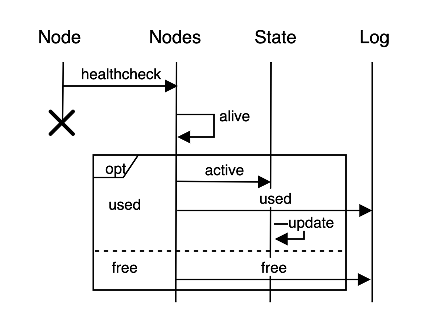
\includegraphics[scale=0.75]{images/FIG2}
	\end{center}
	\vspace{-0.7cm}
	\caption{Low level health-check protocol diagram.}
	\label{fig:fig6}
\end{figure} 

\noindent
These participants included in Figure~\ref{fig:fig6} follow the health-check protocol~\label{informal_description_health-check} that is informally described below:

\begin{enumerate}[start=1,label={(\bfseries \arabic*)}]
	\item \textbf{Node} sends a health-check signal to the Nodes service;
	\item \textbf{Nodes} accept health-check signals from every node, update node metrics and if node is used in some cluster, inform that cluster about the node state;
	\item \textbf{State} contains information about nodes in the clusters, regions and topologies;
	\item \textbf{Log} contains records of operations. Users can query this service. 
\end{enumerate}

\noindent
Nodes service will be informed about node existence on his health-check ping. However, the system state will not be updated, changed, or even informed about this ping if the node is not used in some cluster.

In the following algorithm~\ref{alg:alg1} steps required by the system to determine if the node is free or used, and how node information is stored, are described.

\begin{algorithm}[H]
	\SetAlgoLined
	\SetKwInOut{Input}{input}
	\Input{event, config}
	\uIf{isNodeFree(event.id)}{
		\eIf{exists(event.id)}{
			renewLease(event.id, config.leaseTime)\;
			updateData(event.id, event.data)\;
		}{
			leaseNewNode(event.id, config.leaseTime, event.data)\;
			saveMetrics(event.id, event.metrics)\;
		}
	}\uElseIf{isNodeReserved(event.id)}{
		updateData(event.id, event.data)\;
	}\Else{
		renewLease(event.id, config.leaseTime)\;
		updateData(event.id, event.data)\;
		saveMetrics(event.id, event.metrics)\;
		sendNodeACK(event.id)\;
	}
	\caption{Health-check data received}
	\label{alg:alg1}
\end{algorithm}

\noindent
To formally describe servers or nodes (terms are used interchangeably) properties in the system, set theory could be used. At the beginning, the system will have an empty server set $S$ denoted with $S=\emptyset$. To determine node state, we could use existing node properties. One approach may be that we use a node-id structure, for example. 

Whatever approach is used, free nodes can be formally described as follows:

\begin{definition}
	Nodes are free if and only if (henceforth iff) they do not belong to any cluster.
\end{definition}

\noindent 
If \textbf{node-id} is taken, for example, when the new health-check message from the particular node is received, \textbf{node-id} structure will determine the node state. When the node is free, it will home some random or user-defined id, while when it is used in some cluster, the node-id structure will reflect this.\\

If, for example, there are $n$ free nodes in the wild, this can be denoted with $s_i$, where $i\in\{1, \ldots, n\},$. If all of them send the health-check ping to the system, we need to determine their state. If a node $s_i$ is free, we should add it to the server set, and thus we have:

\begin{equation}
	S_{\mathit{new}} = S_{\mathit{old}} \cup \bigcup%\limits
	_{i=1}^{n} \{s_i\}
\end{equation}
\myequations{Extending free servers set.}
 
\noindent 
It is important to notice, that the order in which messages arrive is not important. The only thing that is important is that every message eventually comes into the system. Node roles in the system can now formally be defined like:

\begin{definition}
	All nodes in the system are equal, no matter if they are a part of some cluster or if they are not.
\end{definition}

\noindent
The previous definition gives us a strong background in the further formal definition of the system because the only thing that should be cared about is that node is alive and well, and that it is ready to accept some jobs.\\

We described in algorithm~\ref{alg:alg1} how the system stores the node data, but also how to determine if the node is free or used using the node-id structure. Every node $s_i$ in the system that is part of the server set $S$ could be described as a tuple $s_i = (L, R, A, I)$, where:

\begin{itemize}
	%
	%
	\item $L$ is a set of ordered key-value pairs, i.e., $L = \{(k_1,v_1),\ldots ,(k_m,v_m)\}$ where $k_i \not= k_j$, for each $i,j\in \{1, \ldots , m\}$ such that $i\not= j$. $L$ represents node labels or server-specific features.  
	Labels were based on Kubernetes~\cite{RossiCPN20} labels concept, which is used as an elegant binding mechanism for its components.
	%
	%
	\item $R$ is a set of tuples $R = \{(f_1,u_1,t_1),\ldots ,(f_m,u_m,t_m)\}$ representing node resources, where $f_i,u_i,t_i$, for $i\in\{1,\ldots,m\}$ are as follows:
	\begin{itemize}
		\item $f_i$ is the free resource value, 
		\item $u_i$ is the used resource value, and 
		\item $t_i$ is the total resource value. 
	\end{itemize}
	%
	%
	\item $A$ is a set of tuples $A = \{(l_1,r_1,c_1,i_1), \ldots ,(l_m,r_m,c_m,i_m)\}$, representing running applications, where $l_j,r_j,c_j,i_j$, for $j\in\{1,\ldots,m\}$, are as follows: 
	\begin{itemize}
		\item  $l_j$ represents labels, the same way we used for node labels, 
		\item $r_j$ is the resource set application requires, 
		\item $c_j$ is the configuration set application requires, and 
		\item $i_j$ is the general information like name, port, developer. 
	\end{itemize}
	%
	%
	\item $I$ represents a set of general node information like: name, location, IP address, id, cluster id, region id, topology id, etc.
\end{itemize}

\noindent
If we want to assign $m$ (fresh) labels to the $i_\mathit{th}$ server, we start with empty labels set $s_i[L]=\emptyset$, then we add labels to server. Therefore, we have 

\begin{equation}
	s_i[L]_\mathit{new} = s_i[L]_\mathit{old} \cup \bigcup%\limits
	_{j=1}^{m} \{(k_j,v_j)\
\end{equation}
\myequations{Extending label set.}

\noindent
We can now formally define the number of labels per single server $s_i$ in the system like:

\begin{definition}
	Every node from the server set $S$ \textbf{must have} \emph{non-empty} set of labels. The number of labels for every server $s_i$ in the server set $S$ may vary.
\end{definition}

\noindent
Since labels are an important part of the system (more in future sections), they should be picked carefully and agreed on upfront. It should also be possible to change them if such a thing is required. 

Labels should stick out some distinctive features of the node, that might be valuable for developers or administrators to target. For example, server resources, server features (e.g., SSD drive), geolocation, etc. They can be created as follows:

\begin{definition}
	Labels are created using arbitrary long alphanumeric text, for both keys and values, separated by colon sign. For example os:linux, arch:arm, model:rpi, cpu:$2$, memory:$16$GB, disk:$300$GB, etc.
\end{definition}

\noindent
Following all things presented above, we can now give a formal description for the low-level health-check communication protocol (cf. Figure~\ref{fig:fig6}). The global protocol $\G_1$ (given bellow) conforms the informal description given at page~\pageref{informal_description_health-check}: $\mathtt{node}$ connects $\mathtt{nodes}$ with $\mathit{health{\_}check}$ message and a payload of type $\T_1$ required by the system to properly register node into the system. 

Based on the received information, $\mathtt{nodes}$ {\bf either} connect $\mathtt{state}$ with $\mathit{active}$ message, informing the node status alongside payload typed with $\T_2$ (containing informations required by the system to properly register active health-check sender), and then also connect $\mathtt{log}$ with the same message, {\bf or} directly connect $\mathtt{log}$ informing the node is $\mathit{free}$.
\begin{align*}
\G_1 = & 
\mathtt{node} \twoheadrightarrow \mathtt{nodes}{:}\mathit{health{\_}check}(\T_1).\\
& \hspace{2mm}
\left\{
\begin{array}{@{}l@{}}
\mathtt{nodes} \twoheadrightarrow \mathtt{state}{:}\mathit{active}(\T_2).\mathtt{nodes}\twoheadrightarrow \mathtt{log}{:}\mathit{used}(\T_2).\tend\\
\mathtt{nodes}\twoheadrightarrow \mathtt{log}{:}\mathit{free}(\T_2).\tend
\end{array} \right.
\end{align*}
\myequations{Health-check global protocol.}

Notice that in $\G_1$ we indeed have a choice of $\mathtt{nodes}$ sending either to $\mathtt{state}$ or to $\mathtt{log}$. Such communication patterns are impossible to be modeled using just standard MPST approaches. 
Also, notice that $\mathtt{state}$ will be introduced into the session only when receiving from $\mathtt{nodes}$. 
Hence, if the session after the first ping from $\mathtt{node}$ to $\mathtt{nodes}$ proceeds with the second branch (i.e., connecting $\mathtt{nodes}$ with $\mathtt{log}$) then $\mathtt{state}$ is not considered as stuck, as it would be in standard MPST, such as, e.g.,~\cite{HondaYC08}, but rather idle. 

Projecting global type $\G_1$ onto participants $\mathtt{node}, \mathtt{nodes}, \mathtt{state}$ and $\mathtt{log}$ we can then get local types as follows:
\begin{align*}
\ST_\mathtt{node}  & = 
\mathtt{nodes}{!!}\mathit{health{\_}check}(\T_1).\tend
\end{align*}
\begin{align*}
\ST_\mathtt{nodes} & = 
\mathtt{node}{??}\mathit{health{\_}check}(\T_1). \\
& \hspace{-2mm}
{+} 
\left\{
\begin{array}{@{}l@{}}
\mathtt{state}{!!}\mathit{active}(\T_2).\mathtt{log}{!!}\mathit{used}(\T_2).\tend\\
\mathtt{log}{!!}\mathit{free}(\T_2).\tend
\end{array} \right.
\end{align*}
\begin{align*}
\ST_\mathtt{state} &= 
\mathtt{nodes}{??}\mathit{active}(\T_2).\tend
\end{align*}
\begin{align*}
\ST_\mathtt{log} &= 
{+}
\left\{
\begin{array}{@{}l@{}}
\mathtt{nodes}{??}\mathit{used}(\T_2).\tend\\
\mathtt{nodes}{??}\mathit{free}(\T_2).\tend
\end{array} \right.
\end{align*}
\myequations{Health-check global protocol projection.}
\noindent
where, for instance, type $\ST_\mathtt{nodes}$ specifies $\mathtt{nodes}$ can receive the ping message from $\mathtt{node}$, after which it will dynamically introduce either $\mathtt{state}$ or $\mathtt{log}$ into the session, where in the former case it also connects $\mathtt{log}$ (but now with message $\mathit{free}$). 
%
%
\subsection{Cluster formation protocol}\label{sec:cluster_formation_protocol}
%
Another communication protocol that the system relies on, appears in the cluster formation process, where users can form new clusters dynamically. Two different actions are distinguished:

\begin{enumerate}[start=1,label={(\bfseries \arabic*)}]
	\item The first action is user-system communication. Here user sends query parameters to the system to obtain a list of available nodes that satisfy specified query parameters.
	\item The second action is a little bit more complicated than the previous one, and it starts when the user sends a message to the system with a new assembly specification. In this setting, the system involves participants: User, Queue, Scheduler, State, Nodes, Log, and NodesPool. These participants need to cooperate to successfully form new clusters, regions, or topologies dynamically, adhering to the scenario shown in Figure \ref{fig:fig7}.
\end{enumerate} 

\begin{figure}[H]
	\begin{center}
		\includegraphics[scale=0.7]{images/FIG3}
	\end{center}
	\vspace{-0.7cm}
	\caption{Low level cluster formation communication protocol diagram.}
	\label{fig:fig7}
\end{figure}

\noindent
These participants included in Figure~\ref{fig:fig7} follow the cluster formation protocol that is informally described below:

\begin{enumerate}[start=1,label={(\bfseries \arabic*)}]
	\item \label{cluster_formation_informal_description} \textbf{User} query Nodes service, based on some predefined query parameters. User sends a new creation message to Queue. User either gets response \textit{ok} if the message is accepted or \textit{error} if the message cannot be accepted due to missing rights or other issues. This operation is called \emph{mutation}; 
	\item \textbf{Queue} accepts a user message, and passes it to State. Messages are handled in FIFO (First In, First Out) order. The queue prevents system congestion, with received messages. The queue will also test if the specified message has already been handled before over idempotency check;
	\item \textbf{State} accepts mutation messages from Queue, and tries to store new information about the cluster, region, or topology. If Nodes can reserve all desired nodes, the system  will store new user desired specification and send a message to Scheduler to physically carry on the creation of clusters with desired nodes;
	\item \textbf{Nodes} accept messages from State. It will reserve desired nodes, if possible, otherwise, it will send an error message to Log service. On a health-check message, it will either just store node information or if a node is used in some cluster, inform that cluster that the node is alive;
	\item \textbf{Scheduler} waits for a message sent from State, and physically carry on cluster formation by pushing cluster formation messages to the chosen nodes;
	\item \textbf{Log} contains records of all operations. Users can query this service to see if their tasks are finished or some problems occurred;
	\item \textbf{Nodes Pool} represents the set of \emph{n} free nodes that will accept mutation messages. When a node receives the message, it will follow some predefined steps:
	
	\begin{enumerate}[start=1,label={(\bfseries \roman*)}] 
		\item start gossip protocol to inform other nodes from the mutation message that they should form a cluster;
		\item when cluster formation is done, send an event to Scheduler and Nodes that node is alive and can receive messages. The cluster formation is done, when all nodes have complete list of nodes that should form the cluster;
	\end{enumerate}
\end{enumerate}

\noindent
If a user wants to get a list of free nodes in the system, he must create a query using \emph{the selector}, which is the set of key-value pairs where he can describe what type of nodes he desires. Algorithm~\ref{alg:alg2} describes steps that are required to perform a proper node lookup based on a received selector value.

\begin{algorithm}[H]
	\SetAlgoLined
	\SetKwInOut{Input}{input}
	\Input{query}
	Initialize: nodes $\leftarrow$ []\\
	\ForEach{node $\in$ freeNodes()}{
		\If{len(node.labels) == len(query) $\land$ node.haveAll(query)}{
			nodes.append(node)\\
		}
	}
	\Return nodes
	\caption{Nodes lookup}
	\label{alg:alg2}
\end{algorithm}

We start with the empty selector $Q=\emptyset$, in which we append key-value pairs. Hence, when a user submits a set of $p$ key-value pairs we have that 

\begin{equation}
	Q_\mathit{new} = Q_\mathit{old} \cup \bigcup%\limits
	_{i=1}^{p} \{(k_i,v_i)\
\end{equation}
\myequations{Query selector formation.} 

\noindent
Once the user submits query selector to the system with desired attributes, for every server in the set $S$, two things need to be checked:

\begin{enumerate}[start=1,label={(\bfseries \arabic*)}]
	\item the cardinality of the $i_\mathit{th}$ server's set of labels and the query selector are identical in size
	\begin{equation}
	\left|s_i[L]\right|=\left|Q\right|, \text{ and } \label{eq:eq1}
	\end{equation}
	\item every key-value pair from query set $Q$ is present in the $i_\mathit{th}$ server's labels set $s_i[L]$, hence the following predicate must yield true:
	\begin{equation}
	P(Q, s_i)= \Big( {\forall}(k,v){\in} Q \,{\exists} (k_j,v_j){\in} s_i[L] \text{ such that }  k=k_j \wedge v\leq v_j \Big) \label{eq:eq2}
	\end{equation}
\end{enumerate} 

The $i_\mathit{th}$ server from the server set $S$ will be present in the result set $R$, iff both rules are satisfied so we have:

\begin{equation}\label{frm:query_rule}  
	R=\{ s_i \;|\; \left|s_i[L]\right|=\left|Q\right| \wedge P(Q, s_i),i\in\{1, \ldots, n\}\}
\end{equation} 
\myequations{Server selector.}

\noindent
If the result set $R$ is not the empty set, we then reserve nodes for configurable time so that other users cannot see, and try to use them.  Finally, reserved nodes with message data $\mathit{md}$ are added to the task queue set:

\begin{equation}
	TQ_\mathit{new} =TQ_\mathit{old}\cup \{(R, md)\}.
\end{equation}
\myequations{Extending task queue set.}

\noindent 
When the task comes to execution, the task queue will send messages to every node that is specified. Algorithm~\ref{alg:alg3} describes the steps required for cluster formation.

\begin{algorithm}[H]
	\SetAlgoLined
	\SetKwInOut{Input}{input}
	\Input{request, config}
	nodes $\leftarrow$ searchFreeNodes(data.query)\\
	reserveNodes(nodes, config.time)\\
	pushMsgToQueue(nodes, data)\\
	key $\leftarrow$ saveTopologyLogicState(data)\\
	watchForNodesACK(key)\\
	\caption{Clustering formation message}
	\label{alg:alg3}
\end{algorithm}

\noindent
Users are free to override existing node labels with their labels or keep predefined ones when including nodes in the cluster. If the node is free, or the user did not change the node labels on cluster formation, the system will use default labels like node geo-location, resources, operating system, architecture, etc.   

When the node receives the cluster formation message, he will automatically pick and contact a configurable subset of nodes $R_g \subset R$, and start the gossip protocol, propagating pieces of information about nodes in the cluster (e.g, new, alive, suspected, dead, etc.). When every node inside the newly formed cluster has a complete set of nodes $R$ obtained through gossiping, the cluster formation process is over. Topology, region, or cluster formation should be done descriptively using YAML, or similar formats. 

In the Algorithm~\ref{alg:alg4} describes the required steps after nodes receive a cluster formation message.

\begin{algorithm}[H]
	\SetAlgoLined
	\SetKwInOut{Input}{input}
	\Input{event}
	\Switch{event.type}{
		\Case{formationMessage}{
			updateId(event.topology, event.region, event.cluster)\\
			newState $\leftarrow$ updateState(event.labels, event.name)\\
			sendReceived(newState)\\
			nodes $\leftarrow$ pickGossipNodes(event.nodes)\\
			startGossip(nodes)
		}
	}
	\caption{Node reaction to clustering message}
	\label{alg:alg4}
\end{algorithm}

\noindent
In the following, a low-level cluster formation communication protocol (cf. Figure \ref{fig:fig3}) is described. We are using the same extension of MPSTs~\cite{HuY17} used for the health-check protocol.

Global protocol $\G_2$ (given below) conforms the informal description of the cluster formation protocol given on page~\pageref{cluster_formation_informal_description}. 
The protocol starts with $\mathtt{user}$ connecting $\mathtt{state}$ by message $\mathit{query}$ and a payload typed with $\T_1$ that contains user query data, and  then $\mathtt{state}$ forwards the message by connecting $\mathtt{nodes}$. 
Then, the protocol possibly enters into a loop, specified with $\mu\ty$, depending on the later choices. 
Further, $\mathtt{nodes}$ replies a response $\mathit{resp}$ to $\mathtt{state}$, that, in turn, forwards the message to $\mathtt{user}$. The payload of the message is typed with $\T_2$ that has response data, based on a given query. 
At this point, $\mathtt{user}$  sends to $\mathtt{state}$ one of three possible messages:

\begin{enumerate}[start=1,label={(\bfseries \arabic*)}]
	\item $\mathit{mutate}$, and the mutation process, described with global protocol $\G'$, starts; 
	\item $\mathit{quit}$, in which case the protocol terminates; or,
	\item $\mathit{query}$ -- this means the process of querying starts again, the query message is forwarded to $\mathtt{nodes}$ and the protocol loops, returning to the point marked with $\mu\ty$.
\end{enumerate}

\noindent
The third branch is the only one in which protocol loops. Also, we can notice that $\mathtt{user}-\mathtt{state}$ and $\mathtt{state}-\mathtt{nodes}$ are connected before specifying recursion. Hence, even after several recursion calls, these connections will be unique. So it is not required to disconnect them before looping.   
\begin{align*}
\G_2 = & 
\mathtt{user} \twoheadrightarrow \mathtt{state}{:}\mathit{query}(\T_1).
\mathtt{state}\twoheadrightarrow \mathtt{nodes}{:}\mathit{query}(\T_1). \\
& \hspace{2mm}
\mu \ty.
\mathtt{nodes}\to \mathtt{state}{:}\mathit{resp}(\T_2).
\mathtt{state}\to\mathtt{user}{:}\mathit{resp}(\T_2). \\
& \hspace{4mm}
\left\{
\begin{array}{@{}l@{}}
\mathtt{user}\to\mathtt{state}{:} \mathit{mutate}().\G'\\
\mathtt{user}\to\mathtt{state}{:} \mathit{quit}().\tend\\
\mathtt{user}\to\mathtt{state}{:} \mathit{query}(\T_1).\mathtt{state}\to\mathtt{nodes}{:}\mathit{query}(\T_1).\ty
\end{array} \right.
\end{align*}
\myequations{Cluster formation global protocol.}

\noindent
The mutate protocol $\G'$, activated in the first branch in $\G_1$, starts with $\mathtt{user}$ sending 
$\mathtt{create}$ message to $\mathtt{state}$, specifying also information about new user desired state typed with $\T_3$, 
and $\mathtt{state}$ replies back with $\mathit{ok}$. 
Then, $\mathtt{state}$ sends $\mathit{ids}$ of the nodes to be reserved (specified in the payload typed with $\T_4$) to $\mathtt{nodes}$, that, in turn sends one of the two possible messages to $\mathtt{state}$: 

\begin{enumerate}[start=1,label={(\bfseries \roman*)}]
	\item $\mathit{rsrvd}$, denoting all nodes are reserved and the protocol proceeds as prescribed with $\G''$, or
	\item $\mathit{error}$, with error message in the payload, informing there has been unsuccessful reservation of nodes, in which case $\mathtt{state}$ connects $\mathtt{log}$ reporting the error and the protocol terminates.
\end{enumerate}

\noindent
\begin{align*}
\G' = & 
\mathtt{user} \to \mathtt{state}{:}\mathit{create}(\T_3).
\mathtt{state} \to \mathtt{user}{:}\mathit{ok}().\\
& \hspace{2mm}
\mathtt{state}\to\mathtt{nodes}{:}\mathit{ids}(\T_4). \\
& \hspace{4mm}
\left\{
\begin{array}{@{}l@{}}
\mathtt{nodes}\to \mathtt{state}{:}\mathit{rsrvd}().\G''\\
\mathtt{nodes}\to \mathtt{state}{:}\mathit{err}(\mathsf{String}).\mathtt{state}\twoheadrightarrow\mathtt{log}{:}\mathit{err}(\mathsf{String}).\tend
\end{array} \right.
\end{align*}

\noindent
Finally, in $\G''$ $\mathtt{state}$ connects $\mathtt{sched}$ (Scheduler) with message $\mathit{ids}$ and the payload that contains other data imported for mutation to be completed (typed with $\T_5$). 
Then, $\mathtt{sched}$ connects $\mathtt{pool}$ (Nodes Pool) with $\mathit{update}$ specified with $\T_6$, after which $\mathtt{pool}$ replies back with $\mathit{ok}$, and connects to $\mathtt{nodes}$ sending new id's $\mathit{nids}$ typed with $\T_4$ ( that contains successfully reserved user desired nodes). Now $\mathtt{nodes}$ notifies $\mathtt{state}$ the action was successful, that in turn connects $\mathtt{log}$ with the same message, and the protocol terminates.
\begin{align*}
\G'' = &
\mathtt{state}\twoheadrightarrow\mathtt{sched}{:}\mathit{ids}(\T_5).
\mathtt{sched}\twoheadrightarrow\mathtt{pool}{:}\mathit{update}(\T_6). \\
& \hspace{-2mm}
\mathtt{pool}\to\mathtt{sched}{:}\mathit{ok}(). \\
& %\hspace{2mm}
\mathtt{pool}\twoheadrightarrow\mathtt{nodes}{:}\mathit{nids}(\T_4). 
\mathtt{nodes}\to\mathtt{state}{:}\mathit{succ}(). \\
& \hspace{2mm}
\mathtt{state}\twoheadrightarrow \mathtt{log}{:}\mathit{succ}().\tend
\end{align*}
We may now obtain the projections of global type $\G_2$ onto the participants $\mathtt{user}, \mathtt{state}, \mathtt{nodes}$, $\mathtt{log}$, $\mathtt{pool}$, and $\mathtt{sched}$:
\begin{align*}
\ST_\mathsf{user} = & 
\mathtt{state}{!!}\mathit{query}(\T_1).\mu \ty. 
\mathtt{state}{?}\mathit{resp}(\T_2).\\
& \hspace{2mm}
{+}
\left\{
\begin{array}{@{}l@{}}
\mathtt{state}{!}\mathit{mutate}().\mathtt{state}{!}\mathit{create}(\T_3).\mathtt{state}{?}\mathit{ok}().\tend\\
\mathtt{state}{!}\mathit{quit}().\tend\\
\mathtt{state}{!}\mathit{query}(\T_1).\ty
\end{array} \right.
\end{align*}
\begin{align*}
	\ST_\mathsf{state} = &
	\mathtt{user}{??}\mathit{query}(\T_1).
	\mathtt{nodes}{!!}\mathit{query}(\T_1). %\\
	%& \hspace{2mm}
	\mu \ty. 
	\mathtt{nodes}{?}\mathit{resp}(\T_2).\\
	& \hspace{-4mm} 
	\mathtt{user}{!}\mathit{resp}(\T_2).\\
	& \hspace{-10mm}
	{+}
	\left\{
	\begin{array}{@{}l@{}}
	\mathtt{user}{?}\mathit{mutate}().\mathtt{user}{?}\mathit{create}(\T_3).\mathtt{user}{!}\mathit{ok}().
	\mathtt{nodes}{!}\mathit{ids}(\T_4).\ST'\\
	\mathtt{user}{?}\mathit{quit}().\tend \\
	\mathtt{user}{?}\mathit{query}(\T_1).\mathtt{nodes}{!}\mathit{query}(\T_1).\ty
	\end{array} \right.
\end{align*}
where
\begin{align*}
	\ST' = &
	{+}
	\left\{
	\begin{array}{@{}l@{}}
	\mathtt{nodes}{?}\mathit{rsrvd}().\mathtt{sched}{!!}\mathit{ids}(\T_5).\mathtt{nodes}{?}\mathit{succ}().\mathtt{log}{!!}\mathit{succ}().\tend\\
	\mathtt{nodes}{?}\mathit{err}(\mathsf{String}).\mathtt{log}{!!}\mathit{err}(\mathsf{String}).\tend
	\end{array} \right.
\end{align*}
\begin{align*}
	\ST_\mathtt{nodes} =  &
	\mathtt{state}{??}\mathit{query}(\T_1).
	\mu \ty.
	\mathtt{state}{!}\mathit{resp}(\T_2).\\
	& \hspace{-14mm}
	{+}
	\left\{
	\begin{array}{@{}l@{}}
	\mathtt{state}{?}\mathit{ids}(\T_4).
	{+}\left\{
	\begin{array}{@{}l@{}}
	\mathtt{state}{!}\mathit{rsrvd}().\tend\\
	\mathtt{state}{!}\mathit{err}(\mathsf{String}).\mathtt{poll}{??}\mathit{nids}(\T_4).\\
	\mathtt{state}{!}\mathit{succ}().\tend
	\end{array} \right.	\\
	\mathtt{state}{?}\mathit{query}(\T_1).\ty
	\end{array} \right.
\end{align*}
\begin{align*}
	\ST_\mathtt{log} =& 
	{+}
	\left\{
	\begin{array}{@{}l@{}}
	\mathtt{state}{??}\mathit{succ}().\tend\\
	\mathtt{state}{??}\mathit{err}(\mathsf{String}).\tend
	\end{array} \right.
\end{align*}
\begin{align*}
	\ST_\mathtt{pool} =&
	\mathtt{sched}{??}\mathit{update}(\T_6).
	\mathtt{sched}{!}\mathit{ok}(). 
	\mathtt{nodes}{!!}\mathit{nids}(\T_4).\tend
\end{align*}
\begin{align*}
	\ST_\mathtt{sched} =& 
	\mathtt{state}{??}\mathit{ids}(\T_5).
	\mathtt{pool}{!!}\mathit{update}(\T_6).
	\mathtt{pool}{?}\mathit{ok}().\tend
\end{align*}
\myequations{Cluster formation global protocol projection.}

\noindent
For instance, type $\ST_\mathtt{sched}$ specifies that participant $\mathtt{sched}$ gets included in the session only after receiving from $\mathtt{state}$ message $\mathit{ids}$, then $\mathtt{sched}$ connects $\mathtt{pool}$ with $\mathit{update}$ message, after which it expects to receive $\mathit{ok}$ message and finally terminates. 

We remark that global type $\G_2$ could also be modeled directly by using standard MPST models (such as~\cite{HondaYC08}). However, in such models, the projection of $G_2$ onto, for instance, participant $\mathtt{sched}$ would be undefined (cf.~\cite{HuY17}).
Since we follow the approach of~\cite{HuY17} with explicit connections, projection of $\G_2$ onto $\mathtt{sched}$ is indeed defined as $\ST_\mathtt{sched}$.
%
%
\subsection{Idempotency check protocol}\label{sec:idempotency_protocol}
%
Mutate operation should be atomic, immutable, and idempotent. The user can specify the same topology details but in a different order, for example. We must ensure that the new cluster formation protocol should \textbf{not} be initiated, if the user changes order of regions, clusters, nodes, or labels in one or more node/s. 

If mutate operation fails, for whatever possible reason, but the infrastructure is created, or the same infrastructure already exists, the user should get a message that infrastructure is formed. If the user changes the number of labels per node, nodes per cluster, clusters per region \textbf{only} in that case a new protocol should be started.

But since we have a different scenario than standard write to storage, and we do not specify steps on how operations should be done, to implement idempotency correctly we have to do it a little bit differently. First of all, we must ensure that structure and operation that we are going to do over that structure are idempotent.

The idempotent structure can be represented as a tuple of topology name and set of data like $S=(Name, Data)$. $Name$ could be used for faster lookup, while $Data$ can be represented as a set, because most of the set operations are idempotent, as described in SEC. $Data$ set could be represented in two ways:

\begin{enumerate}[start=1,label={(\bfseries \arabic*)}]
	\item \textbf{flat keyspace}, with this option all data could be part of the same set, and distinguishment could be achieved usnig \textit{prefix} identity, for example: region1\_cluster1, cluster1\_node1, \\node1\_label1 etc.
	\item \textbf{hierarhical keyspace}, with this option we can create nested data-structures of elements, for example set of regions, where every region is a set of clusters, where every cluster is a set of nodes, etc. We can go deep as long as we want, but the restriction is that every structure \textbf{must} be idempotent. So we can use a set of sets and so on. With this option, we must test that idempotency is not violated throughout the hierarchy.
\end{enumerate}

\noindent
If we have cached idempotency data for user requests, and if a user tries to send the same request again, we can then test idempotency using set operation \textbf{intersection} because the intersection is an idempotent operation following the next proof.

\begin{proof}\label{def:intersection_idempotent}
	Intersection of two sets $x$ and $y$ $x \cap y$ is an idempotent operation, becasue $x \cap x$ is always equal to $x$. This means that the idempotency law~\ref{form:idempotency_law} $\forall x, x \cap x = x$ is always $true$.
\end{proof}

\noindent
If we have stored user request on cluster formation protocol, and we receive a new request with the same name, \textbf{then} we can take the intersection of two sets. If we get the same set, that means that this action is already done because of the definition~\ref{def:intersection_idempotent}. Otherwise, the request represents the new action, and new cluster formation protocol. 

This can be made a little bit faster, by choosing the proper storage structure. If we first do (the same) topology, the name is already present in the idempotency store, and this lookup will spare us unnecessary comparison on sets. For example, data structures like \emph{Hash tables} store element as pair of $key-value$ and offers time and space complexity for lookups $\mathcal{O}(1)$, \textit{on average}~\cite{0023376}. 

We can go even a little bit further and use CRDTs and SEC to store and replicate data on copidres of the services that are required for the idempotency test.

Figure~\ref{fig:fig13} shows zoomed view in the $State$ participant from figure~\ref{fig:fig7}, and idempotency check communication.

\begin{figure}[H]
	\begin{center}
		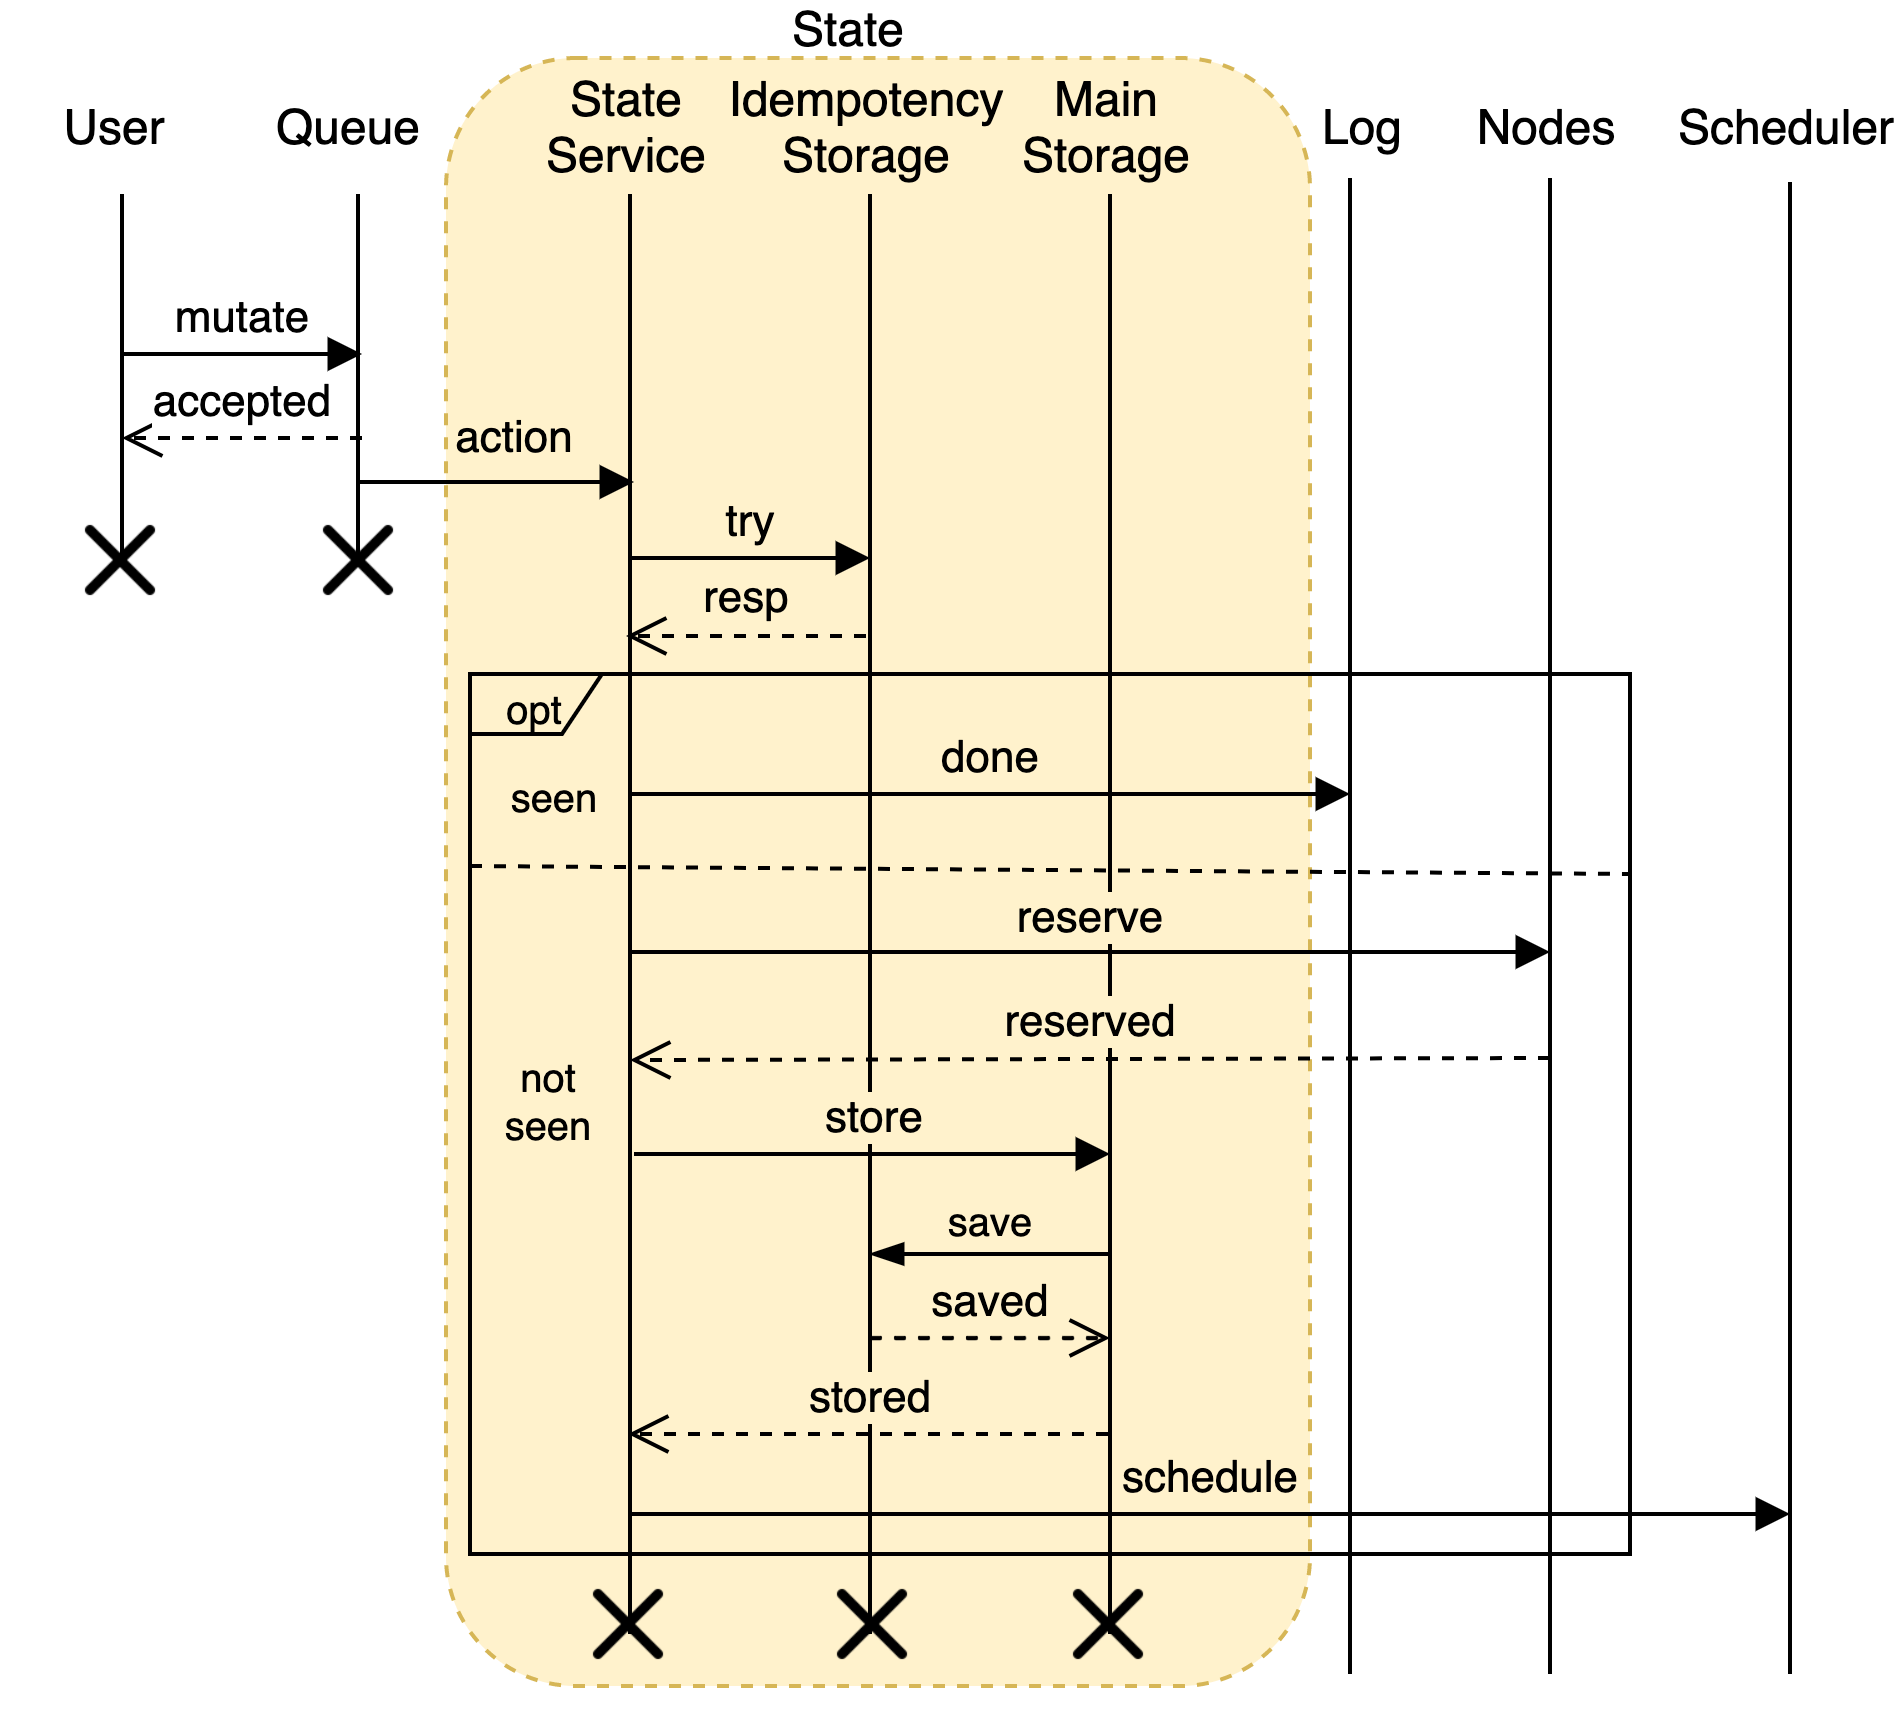
\includegraphics[scale=0.7]{images/Figure13}
	\end{center}
	\vspace{-0.7cm}
	\caption{Low level view of idempotency check communication.}
	\label{fig:fig13}
\end{figure}

\noindent
The participants follow the communication that we now describe informally: \label{informal_description_idempotency}

\begin{enumerate}[start=1,label={(\bfseries \arabic*)}]
	\item \textbf{User} sends a list request to State service (same as~\ref{sec:cluster_formation_protocol});
	\item \textbf{Queue} accepts the list request and the query local state based on the user selector. If a detailed view is required, the state gets metrics data from Nodes service (same as~\ref{sec:cluster_formation_protocol});
	\item \textbf{State service} is a wrapper aroud system main storage. Interacts with main storage in order to create new topologies, regions or clusters, or to get data from the main storages about the same entities. 
	\item \textbf{Idempotency storage} contains idempotent set for all \textbf{already} formed topologies, regions and clusters.
	\item \textbf{Main storage} contains records about the desired state for all formed topologies, regions, and clusters.
	\item \textbf{Log} contains records of operations. Users can query this service to see if their tasks are finished or have any problems (same as~\ref{sec:cluster_formation_protocol});
	\item \textbf{Nodes} accept messages from State. If possible, it will reserve desired nodes, otherwise, it will send an error message to Log service. On a health-check message, if a node is used in some cluster, it will inform that the node is alive (same as~\ref{sec:cluster_formation_protocol});
	\item \textbf{Scheduler} waits for a message sent from State, and pushes cluster formation messages to desired nodes (same as~\ref{sec:cluster_formation_protocol});
\end{enumerate}

\noindent
When testing idempotency, we must have in mind that stored structure could be: \textbf{(1)} flat keyspace, and \textbf{(2)} hierarchical keyspace. The both options are valid, as long as the \textbf{structure is idempotent}, and we can do \textbf{idempotent operations} over that structure. For example, $set$ as a data structure and $intersection$ are good candidates. The algorithm that will test structure idempotency must be able to test both options. 

Algorithm~\ref{alg:alg6} describes steps required to test if the operation is done before.

\begin{algorithm}[H]
	\SetKwFunction{idempotent}{idempotent}
	\SetKwProg{Fn}{function}{:}{}
	\Fn{\idempotent{$stored$, $topology$}}{
		\ForEach{data $\in$ topology}{
			\If{isNotSet(data)}{
				\uIf{stored.intersection(data) = stored}{
					\KwRet{true}
				}
				\KwRet{false}
			}
			\Else{\idempotent{$stored, data$}}
		}
	}
	
	\SetAlgoLined
	\SetKwInOut{Input}{input}
	\Input{request}
	id $\leftarrow$ seenBefore(request.payload.name)\\
	\uIf{id = null}{
		return true;
	}\Else{
		stored $\leftarrow$ storage.findRequest(id)\\
		topology $\leftarrow$ request.payload.topology\\
		\KwRet{\idempotent{$stored, topology$}}
	}
	\caption{Mutate idempotency check}
	\label{alg:alg6}
\end{algorithm}

\noindent
A formal description of the idempotency check protocol (cf. Figure~\ref{fig:fig13}) by using~\cite{HuY17} is presented next. The global protocol $\G_3$ (given below) conforms the informal description given at page~\pageref{informal_description_idempotency}. At this point, the $\mathtt{user}$ can choose one of two possible messages: 

\begin{enumerate}[start=1,label={(\bfseries \arabic*)}]
\item $\mathit{quit}$, in which case the protocol terminates; or, 
\item $\mathit{mutate}$, and the mutation process, described with global protocol $\G'$, starts;
\end{enumerate}
\begin{align*}
\G_3 & = 
\left\{
\begin{array}{@{}l@{}}  
\mathtt{user}\to\mathtt{service}{:} \mathit{quit}().\tend\\
\mathtt{user} \to \mathtt{service}{:}\mathit{create}(\T_3).
\mathtt{state} \to \mathtt{user}{:}\mathit{ok}().\G'
\end{array} \right.
\end{align*}
\myequations{Idempotency check global protocol.}

The mutate protocol $\G'$, activated in the first branch in $\G_3$, starts with $\mathtt{user}$ sending 
$\mathtt{create}$ message to $\mathtt{state}$, specifying also information about the new user desired state typed with $\T_3$, 
and $\mathtt{state}$ replies back with $\mathit{ok}$. This process is the same as cluster formation protocol (cf. section~\ref{cluster_formation_informal_description}). Now we start specific communication protocol for idempotency check so $\mathtt{service}$ sends payload $T_3$ to $\mathtt{istorage}$ to test if this request is $seen$ before. The $\mathtt{istorage}$ responds with payload $T_6$ to $\mathtt{service}$, and based on $Boolean$ response $\mathtt{service}$ can do one of two things:

\begin{enumerate}[start=1,label={(\bfseries \arabic*)}]
	\item $\mathtt{service}$ sends message to $\mathtt{log}$ and this process terminates; or,
	\item $\mathtt{service}$ sends $\mathit{ids}$ of the nodes to be reserved (specified in the payload typed with $\T_4$) to $\mathtt{nodes}$;
\end{enumerate}

\noindent
same as cluster formation protocol (cf. section~\ref{cluster_formation_informal_description}). For simplification, we can assume that all nodes are reserved, and now idempotency data store global protocol $\G''$, starts;
\begin{align*}
G' & = 
\mathtt{service} \twoheadrightarrow \mathtt{istorage}{:}\mathit{try}(\T_3). \\
& \hspace{1mm}
\mathtt{istorage} \to \mathtt{service}{:}\mathit{resp}(\mathsf{Boolean}).\\
& \hspace{10mm}
\left\{
\begin{array}{@{}l@{}}
\mathtt{service} \twoheadrightarrow\mathtt{log}{:} \mathit{done}(\mathsf{String}).\tend\\
\mathtt{service} \twoheadrightarrow\mathtt{nodes}{:}\mathit{ids}(\T_4).
\mathtt{nodes} \to \mathtt{service}{:}\mathit{rsrvd}().\G''
\end{array} \right.
\end{align*}

\noindent
The idempotency store protocol $\G''$, starts with $\mathtt{service}$ sending mutation payload $T_3$ to $\mathtt{mstorage}$. Then $\mathtt{mstorage}$ sends the same payload to $\mathtt{istorage}$. When data is saved for future testing, $\mathtt{istorage}$ responds back to $\mathtt{mstorage}$, and finally $\mathtt{mstorage}$ responds back to $\mathtt{service}$. At this point user payload $T_3$ is stored in both main storage and idempotency storage for future testing. Protocol continues with $\mathtt{state}$ connects $\mathtt{sched}$ (Scheduler) with message $\mathit{ids}$ and the payload that contains other data imported for mutation to be completed (typed with $\T_5$), and the rest of cluster formation protocol may continue.

\begin{align*}
\G'' = & 
\mathtt{service} \twoheadrightarrow \mathtt{mstorage}{:}\mathit{store}(\T_3).
\mathtt{mstorage} \twoheadrightarrow \mathtt{istorage}{:}\mathit{save}(\T_3).\\
& \hspace{4mm}
\mathtt{istorage} \to \mathtt{mstorage}{:}\mathit{saved}().
\mathtt{mstorage} \to \mathtt{service}{:}\mathit{stored}().\\
& \hspace{4mm}
\mathtt{service} \twoheadrightarrow \mathtt{sched}{:}\mathit{ids}(\T_5).\tend
\end{align*}

\noindent
We may now obtain the projections of global type $\G_3$ onto the participants $\mathtt{user}, \mathtt{service}, \mathtt{istorage}$, $\mathtt{mstorage}$, $\mathtt{log}$, $\mathtt{nodes}$: and $\mathtt{sched}$:

\begin{align*}
\ST_\mathsf{user} = &
{+}
\left\{
\begin{array}{@{}l@{}}
\mathtt{service}{!}\mathit{quit}().\tend\\
\mathtt{service}{!}\mathit{create}(\T_3).\mathtt{service}{?}\mathit{ok}().\tend\\
\end{array} \right.
\end{align*}
\begin{align*}
	\ST_\mathsf{service} = &
	{+}
	\left\{
	\begin{array}{@{}l@{}}
	\mathtt{user}{?}\mathit{quit}().\tend \\
	\mathtt{user}{?}\mathit{create}(\T_3).\mathtt{user}{!}\mathit{ok}().\ST'\\
	\end{array} \right.
\end{align*}
where
\begin{align*}
	\ST' = &
	\mathtt{istorage}{!!}\mathit{try}(\T_3).\mathtt{istorage}{?}\mathit{resp}(\mathsf{Boolean}).\\
	&
	{+}
	\left\{
	\begin{array}{@{}l@{}}
	\mathtt{log}{!!}\mathit{done}(\mathsf{String}).\tend\\
	\mathtt{nodes}{!!}\mathit{ids}(\T_4).\mathtt{nodes}{?}\mathit{rsrvd}().\ST''\\
	\end{array} \right.
\end{align*}
\begin{align*}
	\ST_\mathtt{mstorage} =  & \hspace{2mm}
	\mathtt{service}{??}\mathit{store}(\T_3).\mathtt{istorage}{!!}\mathit{save}(\T_3).\\ & \hspace{-8mm}
	\mathtt{istorage}{?}\mathit{saved}().\mathtt{service}{!}\mathit{stored}().\tend
\end{align*}
\begin{align*}
	\ST'' = & 
	\mathtt{mstorage}{!!}\mathit{store}(\T_3).\mathtt{mstorage}{?}\mathit{stored}().\\ & \hspace{-8mm}
	\mathtt{sched}{!!}\mathit{ids}(\T_5).\tend
	%\end{align*}
	%
	%\begin{align*}
\end{align*}
\begin{align*}
	\ST_\mathtt{istorage} =  &
	\mathtt{service}{??}\mathit{try}(\T_3).\mathtt{service}{!}\mathit{resp}(\mathsf{Boolean}).\\ & \hspace{-8mm}
	\mathtt{mstorage}{??}\mathit{save}(\T_3).\mathtt{mstorage}{!}\mathit{saved}().\tend
\end{align*}
\begin{align*}
	\ST_\mathtt{log} =  &
	\mathtt{service}{??}\mathit{done}(\mathsf{String}).\tend
\end{align*}
\begin{align*}
	\ST_\mathtt{nodes} =  &
	\mathtt{service}{??}\mathit{ids}(\T_4).\mathtt{service}{!}\mathit{rsrvd}().\tend
\end{align*}
\myequations{Idempotency check global protocol projection.}

\noindent
Similarly, as for $G_2$, we remark $\G_3$ could also be modeled using standard MPST (e.g.,~\cite{HondaYC08}), but again the projection types would be undefined while following the approach of ~\cite{HuY17} with explicit connections, all valid projections have been obtained.
%
%
\subsection{List detail protocol}\label{sec:list_detail_protocol}
%
The final communication protocol in our system appears in the information retrieval process. Using labels, the user can specify what part of the system he wants to retrieve, namely, on formed topologies. This protocol could be useful, for example, if the user wants to visualize his topologies, regions, or clusters on some dashboard and monitor for some changes, alerts, etc. 

This operation may span over multiple services to retreive complete informations about the clusters and/or nodes. For this purpose some of the distributed queries methods (cf.~\ref{sec:distributed_queries}) can be used. For some patterns api composition may be more suited, while for others CQRS may be the better solution to optimize queries.

This protocol comes with two available options: 

\begin{enumerate}[start=1,label={(\bfseries \arabic*)}]
	\item \textbf{global view} of the system -- all topologies the user manages. This will return just basic information about regions and clusters and their utilization.
	\item \textbf{specific clusters} details -- in-depth details for specified clusters like resources utilization over time (using stored metrics information), node information, configuration data, and running or stopped services.
\end{enumerate}

\noindent
It is important to note, that similarly to the query operation (defined previously), both rules $(\ref{eq:eq1})$ and $(\ref{eq:eq2})$ \textbf{must} be satisfied for information to be presented in the response. The user can specify one additional information in the list request, and that is whether or not the user wants a detailed view or not. If such information is presented in the request, the user will get a detaild view back. 

Figure~\ref{fig:fig8} shows a low-level view of the list operation protocol, where users can get details about the formed system. This setting involves the next participants: User, State, Nodes, and Log. 

\begin{figure}[!htbp]
	\begin{center}
		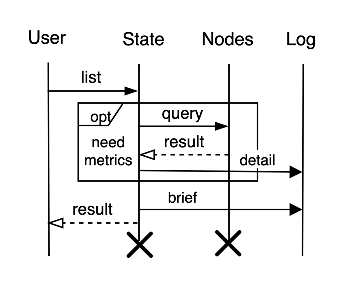
\includegraphics[scale=0.9]{images/FIG4}
	\end{center}
	\vspace{-1.2cm}
	\caption{Low level view of list operation communication.}
	\label{fig:fig8}
\end{figure}

\noindent
Now we can informally describe the roles of the participants in the protocol:\label{list_protocol_informal_description}, shown in figure~\ref{fig:fig8}

\begin{enumerate}[start=1,label={(\bfseries \arabic*)}]
	\item \textbf{User} sends a list request to State;
	\item \textbf{State} accepts the list request and the query local state based on the user selector. If a detailed view is requested, the state gets metrics data from Nodes, and return details back to user;
	\item \textbf{Nodes} contain node metrics data, and if required, it may send this data to State;
	\item \textbf{Log} contains records of all operations. Users can query this service.
\end{enumerate}

\noindent
Algorithm~\ref{alg:alg5} describes steps that are required after the state receives a list message.

\begin{algorithm}[H]
	\SetAlgoLined
	\SetKwInOut{Input}{input}
	\Input{request}
	Initialize: data $\leftarrow$ []\\
	\ForEach{(topology, isDetail) $\in$ userData(request.query)}{
		\uIf{isDetail}{
			data.append(topology.collectData())\\
		}\Else{
			data.append(topology.data())\\
		}
	}
	\Return data
	\caption{List of current state of the system}
	\label{alg:alg5}
\end{algorithm}

\noindent
A formal description of the list communication protocol (cf. Figure \ref{fig:fig4}) by using~\cite{HuY17} is presented next. Global type $\G_4$ (given below) starts with $\mathtt{user}$ connecting $\mathtt{state}$ with one of the two possible messages: 
\textbf{(1)} $\mathit{list}$, specifying a request for a detailed view, where sort $\T_1$ identifies which parts of the system the user wants to view in details, after which $\mathtt{state}$ connects $\mathtt{nodes}$ with $\mathit{query}$ message, with a payload of sort $\T_2$  containing specification of which nodes need to show their metrics data, and then protocol proceeds as prescribed with $\G'$; 
\textbf{(2)} $\mathit{list^*}$, specifies no need for a detailed view is specified, where a payload of sort $\T_4$ denotes user specified parts of the system the user wants to view, but without greater details. In the latter case protocol follows global type $\G''$.
\begin{align*}
\G_4 &= 
\left\{
\begin{array}{@{}l@{}}  
\mathtt{user} \twoheadrightarrow \mathtt{state}{:}\mathit{list}(\T_1).\mathtt{state}\twoheadrightarrow\mathtt{nodes}{:}\mathit{query}(\T_2). \G' \\
\mathtt{user} \twoheadrightarrow \mathtt{state}{:}\mathit{list^*}(\T_4).\G''
\end{array} \right.
\end{align*}
\myequations{List detail global protocol.}
Global type $\G'$ starts with $\mathtt{nodes}$ replying to $\mathtt{state}$ $\mathit{result}$ message and a payload identifying parts of the system user wants to see in greater detail typed with $\T_3$. Then, $\mathtt{state}$ connects $\mathtt{log}$ with $\mathtt{details}$ and also sends $\mathtt{result}$ to $\mathtt{user}$, and finally terminates. 
In $\G''$, $\mathtt{state}$ also connects $\mathtt{log}$ with $\mathit{brief}$ and a payload typed with $\T_5$ identifying parts of the system the user wants to see without greater detail. Then, $\mathtt{state}$ replies to $\mathtt{user}$ with $\mathtt{result}$ message, and the protocol terminates.
\begin{align*}
\begin{split}
	\G' =  & 
	\mathtt{nodes}\to\mathtt{state}{:}\mathit{result}(\T_3).\mathtt{state}\twoheadrightarrow \mathtt{log}{:}\mathit{detail}(\T_3). \\
	& \hspace{2mm}
	\mathtt{state}\to\mathtt{user}{:}\mathit{result}(\T_3).\tend
\end{split}
\end{align*}
\begin{align*}
	\G'' = &
	\mathtt{state}\twoheadrightarrow \mathtt{log}{:}\mathit{brief}(\T_5).\mathtt{state}\to\mathtt{user}{:}\mathit{result}(\T_5).\tend
\end{align*}

\noindent
Same as for the health-check and the cluster formation protocols, here we also present the projections of global type $\G_4$, modeling the list protocol, onto participants $\mathtt{user}$, $\mathtt{state}$, $\mathtt{nodes}$, and $\mathtt{log}$:
\begin{align*}
	\ST_\mathtt{user} =& 
	{+}
	\left\{
	\begin{array}{@{}l@{}}  
	\mathtt{state}{!!}\mathit{list}(\T_1).\mathtt{state}{?}\mathit{result}(\T_3).\tend \\
	\mathtt{state}{!!}\mathit{list^*}(\T_4).\mathtt{state}{?}\mathit{result}(\T_5).\tend 
	\end{array} \right.
\end{align*}
\begin{align*}
	\ST_\mathtt{state} =&
	{+}
	\left\{
	\begin{array}{@{}l@{}}  
	\mathtt{user}{??}\mathit{list}(\T_1).\mathtt{nodes}{!!}\mathit{query}(\T_2).\ST'\\
	\mathtt{user}{??}\mathit{list^*}(\T_4).\mathtt{log}{!!}\mathit{brief}(\T_5).\mathtt{user}{!}\mathit{result}(\T_5).\tend
	\end{array} \right. 
\end{align*}
where
\begin{align*}
	\ST'  =& 
	\mathtt{nodes}{?}\mathit{result}(\T_3).\mathtt{log}{!!}\mathit{detail}(\T_3).\mathtt{user}{!}\mathit{result}(\T_3).\tend
\end{align*}
\begin{align*}
	\ST_\mathtt{nodes} = &
	\mathtt{state}{??}\mathit{query}(\T_2).\mathtt{state}{!}\mathit{result}(\T_3).\tend
\end{align*}
\begin{align*}
	\ST_\mathtt{log} = & 
	{+}
	\left\{
	\begin{array}{@{}l@{}}  
	\mathtt{state}{??}\mathit{detail}(\T_3).\tend \\
	\mathtt{state}{??}\mathit{brief}(\T_5).\tend \\
	\end{array} \right.
\end{align*}
\myequations{List detail global protocol projection.}

\noindent
For instance, type $\ST_\mathtt{log}$ specifies $\mathtt{log}$ gets included in the session only after receiving from $\mathtt{state}$, either message $\mathit{detail}$, or message $\mathit{brief}$, and then terminates. 

Similarly as for $\G_2$ and $\G_3$ we remark $\G_4$ could also be modeled using standard MPST (e.g.,~\cite{HondaYC08}), but again the projection types would be undefined, while following the approach of ~\cite{HuY17} with explicit connections, all valid projections have been obtained.
%
%
\section{Long-lived transactions}\label{sec:long_live_transactions}
%
To operate micro clouds properly, such a system needs to be scalable. Architecture composed of loosely coupled services can be a way to go, because of all benefits such systems offer (cf.~page~\ref{sec:microservices}). But still, we must be aware of all problems that come along with them.

That been said, one of the problems we have to deal with are transactions that appear in such distributed system. Because of the nature of the system \emph{sagas} seems like a better pattern to use (cf. page~\ref{sec:sagas}).

When a user submits the \emph{cluster creation message}, the system will accept the message and register the task with \emph{PENDING} state. If the system cannot proceed further, for whatever reason (no available resources or nodes for example, etc.), such task is done and it goes to \emph{FAILD} state, and this concludes the transaction. Otherwise, if there are no errors, and the system can proceed with the cluster formation protocol, the task will go to \emph{IN PROGRESS} state. 

In this state, the system needs to save newly formed cluster information, prepare metrics service, add watchers for the cluster nodes health-check, and so on. This operation will span over multiple services, and that process can be separated into multiple sub-transactions. The state of the task will prevent the user from submitting other tasks on a cluster that is not formed yet. 

If any error happens during this process, we can always invoke the rollback mechanism, or try to fix the occurred issue with some of the retry strategies.

If the cluster formation is done, and there are no problems occurred the transaction is completed, and the task is moved to \emph{CREATED} state. If some error happens during this process, and a cluster cannot be formed, the task will go again to \emph{FAILD} state, and this concludes the transaction.

Figure~\ref{fig:fig19} shows state diagram for cluster formation message.

\begin{figure}[H]
	\begin{center}
		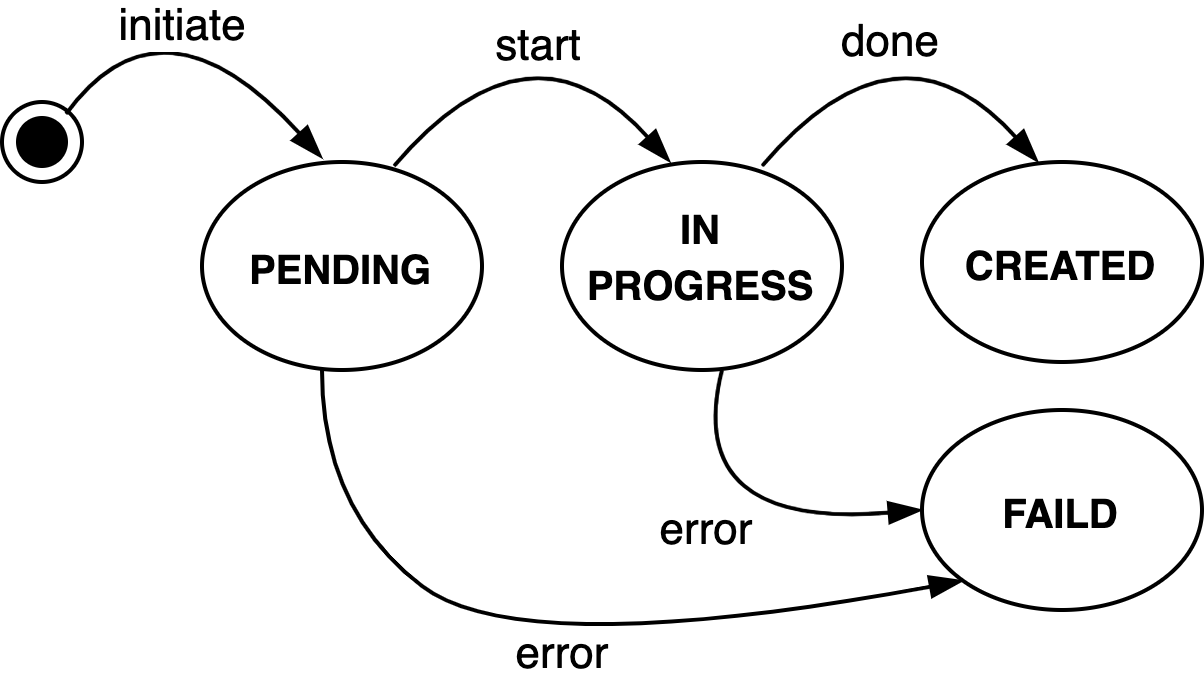
\includegraphics[scale=1]{images/Figure19.png}
	\end{center}
	\vspace{-0.6cm}
	\caption{State diagram for cluster formation message}
	\label{fig:fig19}
\end{figure}

Cluster formation protocol will most likely span over multiple services, and strategies like sagas can be useful to implement transactions and rollbacks properly.
%
%
\subsection{Garbage collection}\label{sec:garbage}
%
When the user submits the task to the system if for whatever reason that task fails we have the option to immediately remove that task, and possibly all task connected items. Or, the system should have a specific process in the background, which the only purpose is the garbage collection to restore unused and fragmented system resources.

The second option seems more acceptable because one item can have a graph of items that are connected to that specific item. This graph can be complex, and immediate deletion may slow down the entire system. In the background, the garbage collection process can mark unused items and delete them when the time is right.

Users should also be able to delete certain items with their dependencies as well, invoking \emph{cascading deletion}. Dependencies may be deleted immediately, or marked as \emph{orphans}, and deleted by the garbage collection process.

It makes sense that users can influence garbage collection by submitting their policies when and how often to do this operation, to delete only items or container images as well, and so on.
%
%
\section{System observability}\label{sec:system_observability}
%
Observability is an importatnt part of any real-world computing system (cf. page~\pageref{sec:log_aggregation}). It is important part of any platform that strive to be offered as a service to large groups of different users. 

At every moment, we must know what is happening in the system, where are bottlenecks and how we can resolve problems. This is of significant importance in DS, where state and calculations are scattered across multiple nodes, clusters and even DCs.

In the micro-clouds environment that involves multile layers (cf. page~\pageref{lab:three-tier}), this technique is even more inportant to give us insight what is happening in the system, and how we can optimize different layers of the system. On the other hands, users who use such system needs to know what is happening with their services.

Because of these two really important parameters, observability myst be implemented on two levels:

\begin{enumerate}[start=1,label={(\bfseries \arabic*)}]
	\item \textbf{system level}, contains data that is generated by the system. This data should be avalible to the administrators and providers of the system \textbf{only}. Operations people in the team (eg. DevOps or SREs), and developers cannot see it.
	\item \textbf{user level} contains informations about user requests that \textbf{only} operations people in the team (eg. DevOps or SREs) should be able see. This type of data should not be visible to the system providers, and for privacy reasons.
\end{enumerate}

\noindent
Every service should log details about its usage and calls as well as traces how requests are going, regardless it is platform or user. Log data should be stored outside the service and the virtualization tool (eg. using sidecar pattern with containers~\cite{BurnsO16}), while pieces of information will be sent to centralized log storage. Sending intervals should be be able to change and adapt for both levels.

Log storage could be searched to see the general state of the system, and pieces of information about user requests and the state of their requests.
%
%
\section{Access pattern}\label{sec:access_pattern}
%
In section~\ref{sec:application_model}, we already discussed system access patterns from the applications point of view, using streams and topics. In this section, we are going to venture into the dashboard and system access described in~\ref{sec:distribution_models}. 

To access the system, requests are going over some \textit{master process}. This process is not responsible for any sort of synchronization, agreement, or something like that, but just to show dashboards and various system details since the cloud is available anywhere in the world, while micro-cloud should serve the local population. 

One question that could come to mind is, what if some cloud provider offering micro-cloud functionality, or running our master process, goes down, should the rest of the micro-clouds go to \textit{read-only} mode and only accept \textbf{read} requests?

All communication is not exclusive to go over that master process, but if the user is nearby to micro-cloud he/she should be able to initiate commands directly to clusters, regions, and topologies. But for dashboards and full pieces of information about his micro-clouds, cloud would be a better solution, just because of more available resources.

If some cloud provider goes down for whatever reason, we should foresee this, and to resolve it, we could use multiple cloud providers using \textit{Multi-Cloud Computing}~\cite{HongDSH19, Ardagna15} so that one cloud provider is a master process and many others are backup in case the whole cloud provider goes down.

We inevitably have some state synchronization here, and we could rely on SEC and CRDTs to do synchronization without some expensive coordination between providers.

This is not generally a problem if applications that are running in micro-clouds are not dependent on some process, location, sensors of services, etc. If this is the case, then we can connect micro-clouds in sort of P2P network and give them some logic to just route request to the proper location on the globe. 

This might not be that fast, since even light is affected by the distance, but we would be able to issue requests to cluster in a different part of the world.
%
%
\section{Repercussion}\label{sec:repercussion}
%
The model presented in this chapter, has three possible execution repercussions:

\begin{enumerate}[start=1,label={(\bfseries \arabic*)}]
	\item \textbf{Stand alone}, the proposed model can serve as a base layer for future ECC as a service implementation. On top of it, we can implement other services and features like scheduling, storage, applications, management, monitoring, etc. As such it could be a viable option in the CC.
	\item \textbf{Integration}, the proposed model could be integrated with existing systems like Kubernetes, OpenShift, or cloud provider infrastructure since they all operate over the cluster. This is possible, with some small infrastructure changes and adaptations because -- the communication should be implemented via standard interfaces like HTTP and JSON, the integrations should be relatively easy to achieve. The proposed model could be used as a geo-distributed description and/or an organization tool.
	\item \textbf{Combination}, this approach can be done over multi-cloud principles. Some cloud tasks could be offloaded to the nearest micro-cloud.
\end{enumerate} 
%
%
\section{Limitations}\label{sec:limitations}
%
Since the perfect model never existed, the model that is proposed in this thesis has some llimitations that we must be aware of, either to work on improvements or use the model as is. When talking about small-scale servers and micro-clouds, we must be aware of a few things.

\begin{enumerate}[start=1,label={(\bfseries \arabic*)}]
	\item We must be aware that not all organizations will be able to deploy micro-clouds, due to the high initial investments required~\cite{MonsalveCC18}. We can rely on government authorities, large cloud providers, or other big companies to build the initial infrastructure for their own needs, and lease it to others similar to the cloud. The general public can use them, similarly to the cloud -- pay as you go, model.
	\item There is no guarantee that existing public cloud providers will allow nodes that are not built, resigned, or deployed by them. If we are building a private cloud, then  we can make a different decision. One way to resolve this issue is that the whole platform becomes open-source so that public cloud providers can engage in the development, and eventually use them as a solution.
	\item These small-scale servers must be out of reach of people and protected in some way so that not everyone has access to them. Some degree of physical security must be implemented.
	\item The places where these small scale servers will be deployed must have a stable internet connection, and the ability to integrate SDN or other similar technologies, so that complex network topologies could be implemented properly.
	\item These servers can have some open architecture or could be custom built by other providers. In both cases, they must be able to satisfy rules that are presented in~\ref{sec:separation_of_concerns}.
	\item Splitting the processing into two parts and the possibility that users can be responsible for micro-clouds may raise some legal concerns. Either to develop interesting applications, use them as a firewall or simply use them as a privacy level for data, there must be a legal agreement that might not be that easy to achieve.
\end{enumerate}
%
%
%!TEX root =  main.tex
\chapter{Implementation}\label{chapter:Implementation}
%
In this chapter, we are going to give more details about the framework implemented based on the formal model and architecture specification given in the previous chapter.

Section~\ref{sec:framework} framework architecture, and system implementation details, and framework limits. In Section~\ref{sec:framework_operations} we present implementation details about framework operations. Section~\ref{sec:app} describe few possible senarios and applications that could utilize micro-clouds platform. In Section~\ref{sec:results} we present results of our experiments.
%
%
\section{Framework}\label{sec:framework}
%
In this section, we are going to introduce an implemented proof-of-concept framework based on the model proposed in the previous chapter~\ref{chapter:Micro_clouds}. The framework is called \textbf{Constellations} or \textbf{c12s}\footnote{https://github.com/c12s} for short because it is strongly influenced by nature and the neverending number of galaxies that the universe is (not only) composed of. Similarly, we are trying to create a universe of clusters that will serve humanity to help them with their day-to-day tasks. The framework is it is open-source, and it is implemented using the microservice architecture with services that have distinct role and purpose to the entire system. These services are:

\begin{itemize}
	\item \textbf{Gateway}, this purpose is to export services feature to the rest of the world. Gateway is designed as a REST service, accepting $JSON$ style messages, so that various clients can communicate to the system. When the request arrives at the gateway, if the request is valid it will pass the request to the rest of the system. It communicate to the rest of the services to check if the user exists, does he have proper rights for actions that he sends, and if not return the proper message and do not propagate it to the rest of the system.
	\item \textbf{Authentification \& Authorization}, the sole purpose of this service is to store users and their credentials. This service will validate does user exists in the system, and does he have certain rights to perform some specific operation. Users that often use the system will be stored in the cache layer of the service so that on the next request his actions are done faster. Users that do not use the system that often will not be stored in the cache, until first use. After that, if the user does not use the system for some time, he will expire from the cache.
	\item \textbf{Queues}, the purpose of this service is to prevent huge request load to the system and to accept more user requests. When the user submits any \textbf{mutation} operation -- an operation that changes the state of the system, these operations will be put in the queue. User can create their queues, to prevent long lines for specific tasks. For example, users can create queues for specific tasks, and use them only for those tasks, while other queues could be general-purpose queues. On system start, every user will start with one queue --- \textbf{default}. When doing mutations on different parts of the system, the user can specify in metadata which queue he wants the task to go to. This service implements a token bucket rate-limiting algorithm~\cite{MathewsKG17} to prevent congestion of the system.
	\item \textbf{Nodes}, this service stores and maintain pieces of information about registered nodes in the system. All node hardware and software details will be stored in this here. This service is also responsible for storing metrics data, accept health-check requests from nodes, and inform the rest of the system that the used node is alive.
	\item \textbf{State}, is the heart of the system. This service stores all information about architecture, clusters, regions, and topologies. When a new cluster/region/topology is created, this service will setup watchers for nodes, so that if the node does not send the health-check signal for some time, that node will be declared dead. This is important so that at any moment we must know the state of the clusters and their utilization. This service as well will cache frequently used nodes data, so that on the next request node lookup is faster since we can have a huge number of nodes, topologies clusters, and pieces of information about them. To prevent data loss, this service will first store a copy of the operation before attempting any mutation of the system.
	\item \textbf{Log}, is responsible for storing all log an trace data from every service. Here user can check are all jobs done, or is there some error and possible why the error happened to resolve it or fix it for the next time. From a user point of view, this is \textbf{read only} service and from a system view, this is \textbf{write only} service.
	\item \textbf{Command push}, the purpose of this service is to push commands and operations to the nodes user desired. This service implements a token bucket rate-limiting algorithm~\cite{MathewsKG17} to prevent constant data push to the nodes. Similar to the state service, this service will store a copy of operation information locally before attempting any push to the nodes. This information will be deleted, once the operation reaches all decided nodes and all of the responses with the acknowledge (ACK) message.
\end{itemize}

\noindent
All services are highly customizable and all have their configuration file that could be changed and adopted. All these services are easy to extend to support new operations and pieces of information about nodes, regions, clusters, topologies, and latter on applications, configurations, namespaces, etc. 

The system operates with four commands, where three of them follow formal models described in the previous chapter. The last command is a simple command to list logs for every user.

Regarding~\ref{sec:access_pattern}, the framework operates as a master process is running in Kubernetes, and through that process, all commands are issued. Future applications can communicate with nodes as stated in~\ref{sec:application_model}. They do not require communication with the master process at all, they can communicate with the formed cluster using topics and streams.

In the rest of this section, we will see details about all operations, as well as used technologies to implement the whole system. We will describe possible applications and give future directions for application development. System architecture is shown in Figure~\ref{fig:fig11}.

\begin{figure}[H]
	\begin{center}
		\includegraphics[scale=0.7]{images/FIG5}
	\end{center}
	\vspace{-0.9cm}
	\caption{Proof of concept implemented system.}
	\label{fig:fig11}
\end{figure}
%
%
\subsection{Technologies}\label{sec:technologies}
%
All services are implemented using the Go\footnote{https://golang.org/} programming language, because of his well-known tooling, support for developing system software, web-based applications, small binaries but also great concurrency model, and ability to build binaries for almost any architecture without any code changes. All services rely on Go implicit \emph{interface} implementation mechanism. Every technology or component used in the system can be swapped for some other, as long as that component implement \emph{interface} fully. The framework is developed in such a way that is relatively easy to extend, or switch and use different components and technologies.

As the main storage layer for our system, we used etcd\footnote{https://etcd.io/}, a popular open-source key-value database, that shows good performance, and it is mostly used for configuration data. Metrics data are stored in the open-source time-series database InfluxDB\footnote{https://www.influxdata.com/}. 

Communication between microservices is implemented in RPC manner using gRPC\footnote{https://grpc.io/}, and Protobuf\footnote{https://developers.google.com/protocol-buffers} as a message definition. gRPC and Protobuf are open-source tools designed by Google to be scalable, interoperable, and available for general purposes. Communication between nodes and the system is carried out using NATS, an open-source messaging system. Health checking and action push to nodes are implemented over NATS\footnote{https://nats.io/} in a publish-subscribe manner.

Caching layer for every service is implemented using Redis\footnote{https://redis.io/} key-value, in-memory database. It is important to notice, that all concrete tools that are used, are easily swappable for some other as long as they implement a proper interface.

All communication with the outside world is done in a REST manner using JSON encoded messages over HTTP. To communicate with the platform, we have developed a simple command-line interface (CLI) application also using the Go programming language that sends JSON encoded messages over HTTP to the system.

Every service is packed in a container, and for this purpose Docker\footnote{https://www.docker.com/} containers are used. To achieve automatic orchestration, and self-heal, and up-time, all services that are packed in containers, are running inside Kubernetes.

Every service will log details about his usage and calls, as well as traces how requests are going. Log data is stored outside the service and container, and pieces of information will be sent to centralized log storage on every $t$ seconds specified by the user. Sending intervals could be changed and adopted using the configuration file for every service independently.

Log data will be stored in the two levels:

\begin{enumerate}[start=1,label={(\bfseries \arabic*)}]
	\item \textbf{system level}, this data is generated by the system and could be viewed by administrators of the system \textbf{only}. Non-operations people in the team or DevOps, but by developers of the system and providers of the system.
	\item \textbf{user level} that stores informations about user requests that \textbf{only} users can see. This type of data will not be visible to the developers of the system, and only users that created these logs will be able to see them.
\end{enumerate}

\noindent
Log storage could be searched to see the general state of the system, and pieces of information about user requests and the state of their requests.
%
%
\subsection{Node daemon}\label{sec:node_daemon}
%
Every node runs a simple daemon program implemented using the Go programming language, as an actor system (Ref. secion~\ref{sec:actor_model}). The actor system is developed for this purpose. When a message arrives, the proper actor will react based on the message type, or discard it if the type is not supported. 

Extending such a system is rather easy because users need to simply write a new actor and logic that goes with them and register it to the system.

When the daemon start, he will first read the configuration file to do the proper setup and then will contact the actor system to start all the actors. 

System messages will be sent to the daemon, but he will not react to these messages. Daemon is not able to communicate with any actor directly. All communication goes through the actor system who is responsible to pass messages to the actors. The actor system at this point has only four existing actors:

\begin{enumerate}[start=1,label={(\bfseries \arabic*)}]
	\item \textbf{cluster actor}, this actor react on messages about new cluster formation, but he is also responsabile to contact rest of the system that message has arrived.
	\item \textbf{internal actor}, this actor react to messages from other actors to update the daemon state. For example on new cluster creation, this actor will update daemon id, name, labels, etc.
	\item \textbf{health actor}, this actor will periodically be sent health-check data to the system about node state, utilization, etc. This actor will communicate to the rest of the hardware to get proper pieces of information, to collect logs from the node, and send all that data to the system.
	\item \textbf{gossip actor}, this actor will communicate with other peers in the group using SWIM protocol techniques.
\end{enumerate}

\noindent
The actor system will monitor these actors, so so that any of the crushes for whatever reason, the actor system will restart them. Listing~\ref{lst:listing3} show the actor system hierarchy of existing actors.

\lstinputlisting[caption={Actor system hierarchy.}, label={lst:listing3}, captionpos=b, xleftmargin=.35\textwidth]{listings/listing3.txt}

\noindent
Before daemon starts, the user needs to specify some parameters for proper configuration like: 

\begin{enumerate}[start=1,label={(\bfseries \arabic*)}] \label{imp:features}
	\item \textbf{identifier}, represent unique identifier of the node. When a node is not part of some cluster this can be whatever the user wants. Once the node is part of some cluster, the identifier will be updated, and it is not advised to change it manually afterward.
	\item \textbf{name}, represent name of the node. This property also can be changed when a node is part of the cluster, otherwise, it can be whatever we want.
	\item \textbf{labels} represent the specific features of the node. Labels are used to query for free nodes, and there is no formal restriction of what they can or can not be. This property can be changed when the node is part of some cluster. It is advised, that as labels we put some specific features of the node that might be beneficial for the user who is looking for nodes to create new cluster/s.
	\item \textbf{health-check details}, here we have pieces of information to control the health-check mechanism. Since nodes communicate with the rest of the system via publish-subscribe events, we must specify the address of the rest of the system and the topic name, where we publish our pieces of information.
	\item \textbf{system information}, represent basic information for a node to know how to contact the rest of the system. We should specify the system address, so that node knows where to send messages, and where are messages are coming from. We can also specify the version of the system we are trying to contact. System version could be used to support \textbf{backward compatibility} if we have multiple API versions of the system running at the same time or some period.
\end{enumerate} 

\noindent
Configuration can be done easily using the YAML configuration file. Listing~\ref{lst:listing1} show simple YAML configuration file for daemon process.

\lstinputlisting[caption={Daemon configiration file}, label={lst:listing1}, captionpos=b, xleftmargin=.35\textwidth]{listings/listing1.yaml}

\noindent
Based on the configuration file, the daemon will start a background health-check mechanism, and it will subscribe to the system, using an identifier as a subscription topic. The background thread will contact the system repeatedly using a contact interval time, specified in the configuration file. 

On every health-check, the node will send labels, names, IDs, and metrics to the system (e.g., CPU utilization, total, used, free ram or disk, etc.). The specified labels will be used when the user is querying for available nodes, while the node id will be used for reservation when forming a cluster.

At the first start of the daemon when the node is free, the user can specify whatever node id he wants. Once, the node is a part of the cluster, the node id will be updated to match that. Node id update will happen on the cluster formation process.
%
%
\subsection{Separation of concerns}\label{sec:framework_SoC}
%
IThe implemented framework follow the clear SoC model, presented in~\ref{sec:separation_of_concerns}. Since the presented model consists of three components, the implemented framework is dealing only with \textbf{resources}~\ref{soc:resources} part of the SoC. 

His job is to organize nodes into clusters, regions, and topologies, to make them communicate and expose their resources to the upper layer of SoC for utilization. The upper layer will run services on these resources, to collect data from data creators and process them as requested.

The upper layer must have set up the infrastructure to do any processing or storage. This middle layer is the binding element between the layers.
%
%
\subsection{Limitations}\label{sec:framework_limits}
% 
The framework at the current state has some limitations that we \textbf{must address}. As shown in figure~\ref{fig:fig11}, for purpose of testing the system, and to give the users any way to interact with the system a CLI application is implemented. This is a good option for initiating commands to the system. The problem with this approach is that showing logs, and topologies might be limiting for users, especially if they monitor and supervise multiple topologies with regions and clusters.

For monitoring, a tool with UI would be a better solution and it can show more details. For a small amount of data when topologies are relatively small, CLI could be used. But for some real-world applications desktop and/or Web-based UI will be a much better solution, and CLI can be used for fast lookup on specific pieces of information about clusters and nodes, for example.

The current implementation of the queueing system is \textbf{limiting} because if we want to extend the system with new queues we need to shut down the whole service, and that is not the best solution. But since the goal of this thesis is not queue management, but micro-cloud formation, protocols, and formal modeling.

But since the purpose of this thesis is not Human-computer interaction, this should be the topic of the future work~\ref{sec:future_work}.
%
%
\section{Operations}\label{sec:framework_operations}
%
In this section, we are going to describe all implemented operations in the framework and present specific details about every individual operation.
%
%
\subsection{Query}\label{sec:query} 
% 
The query operation is used to show all free nodes or filtered free nodes that are registered into the system, to the user (yellow arrows in Figure~\ref{fig:fig11}.). When a user wants to get information about free nodes, they need to submit a \textbf{selector} value which is composed of multiple \textbf{key-value} pairs.  These key-value pairs can be any alphanumeric set of symbols for both keys and values. Based on that key-value pair system will do the query of the free nodes.

The selector will be used as a search mechanism to compare the labels of every free node that exists in the system. The nodes that are satisfying the rules~\ref{frm:query_rule} defined in Section~\ref{sec:cluster_formation_protocol} will be present in the result.

This operation is done before the formation of new topologies, regions, or clusters --- mutation of the system. The user first needs to get a list of free nodes, then he can choose nodes that are best suited for him and try to form topologies, regions, or clusters of them.

The querying process is a little bit changed from one presented in Section~\ref{sec:cluster_formation_protocol}. The only change that is made is the addition of the \emph{Gateway} service that will pass requests into the system and prevent overflow of requests. This change \textbf{does not} affect or validate the formal model presented before. Since the added service does not interfere with the process of searching nodes or changes to the system.

Figure~\ref{fig:fig14} shows a communication diagram for the query action, with the addition of the Gateway service.

\begin{figure}[H]
	\begin{center}
		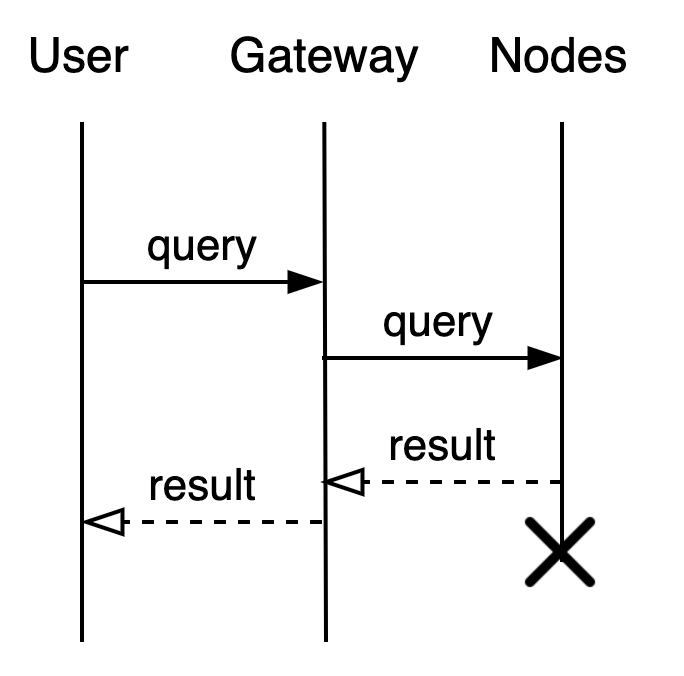
\includegraphics[scale=0.8]{images/Figure14}
	\end{center}
	\vspace{-0.7cm}
	\caption{Low level communication protocol diagram of query operation.}
	\label{fig:fig14}
\end{figure}
%
%
\subsection{Mutate}\label{sec:mutate} 
%
Mutate operation (orange arrows in Figure~\ref{fig:fig11}.) change the system state by creating, editing, or deleting clusters, regions, and topologies. When a user wants to perform a mutation over the system, the desired state needs to be specified \textbf{declaratively} using a YAML file and submitted to the system. When the state is submitted, the system will do the rest of the job to ensure that the state desired by the user is reached.

The users specify which nodes are forming the cluster. Optionally, users can also specify labels and names on the node level, and retention period on the cluster level. The retention period is used to describe how long metrics are going to be kept. When the retention period expires, the metrics data will be deleted or moved to another location. 

When forming a topology, users can assign a name and label to the entire topology. These parameters will be used when the user wants to query all topologies to get full information about regions, clusters, and nodes inside a topology

Mutate operation is \textbf{immutable} which mean that there will be no in-place changes to the existing state. If a user wants to do any update, he needs to specify a full new state that will replace the existing state. This operation is \textbf{atomic} as well, which mean that a whole new state must be able to replace the existing state. If this happens, the system will replace the old state with the new state. The main storage that stores configuration data is a key-value store implemented using an etcd database. The key that will be used to store the configuration data is the whole path of topology, regions, cluster, node, while the value represents the state desired by the user. Listing~\ref{lst:listing4} show structure for key-value pair that is stored in the main database, where on top we can see a structure of the \textbf{key}, and below it we can see the structure of the \textbf{value}. This kind of structure is similar to OS file-system data organizations of files and folders.

\lstinputlisting[caption={Structure of stored key-value element.}, label={lst:listing4}, captionpos=b, xleftmargin=.25\textwidth]{listings/listing4.txt}

\noindent
We store as well one additional information about labels \textbf{index} value. This index is used for a faster query of elements when doing labels comparison. To find elements we can query in a similar way like searching files and folder structure. The etcd in newer version \textbf{do not allow} hierarchical keyspace, but what they allow is \textbf{ranged} query by some \textbf{prefix}. This is useful as well because we can still get all regions in topology, clusters in the region, or nodes in the cluster if we know to which group they belong.

Mutate operation is not idempotent by nature, but the whole process behind it make mutate an idempotent operation. Whether the user tries to create already existing infrastructure by changing the order of regions clusters or labels in the nodes, or if he for whatever reason did not get confirmation that infrastructure is created an existing infrastructure will not be created. This is done in such a way, that $State$ service (Figure~\ref{fig:fig11}) will keep the information set about created infrastructure. This information is implemented as a \textbf{flat keyspace} set, that have information. On every mutation request, the system will test if such a topology already exists. If such topology already exists user will get confirmation that his infrastructure is created. If such topology do not exists, a new cluster formation protocol~\ref{sec:cluster_formation_protocol} will be initiated. The mutation confirmation is followed by a unique id which the user can use to query steps, logs, and traces that are done in process of working towards the state desired by the user. Logs service can give the user complete details about his task state using that unique id.

When creating topologies, the user is free to give whatever name he wants for every region, cluster, and node. The only restriction is that name should be the alphanumeric set of characters. Listing~\ref{lst:listing2} shows an example of a user-defined state that forms the topology of one region with one cluster that contains three nodes, with a retention period of 24 hours. The whole topology will have the same set of labels, but $node3$ redefines this rule by specifying its own.

\lstinputlisting[caption=Example of mutate file using YAML., label={lst:listing2}, captionpos=b, xleftmargin=.3\textwidth]{listings/listing2.yaml}

\noindent
After all, nodes that should form a cluster, acknowledge cluster formation message, they will inform the system that the message is received, and they will start the process of cluster formation. This process is done by using SWIM~\cite{DasGM02}, a Gossip style protocol. When every node has a complete list of his peers that should be in the cluster, the process of cluster formation is done. 

On the next health-check message, every node will send his \textbf{id} that is telling the system that he is part of some cluster. This kind of messages, will be used in the $State$ service to validate that cluster is alive and well, or that some nodes (or all), are dead or down if \textbf{id} is not received. 

And Gossip style protocols (like SWIM) could be used in the future to propagate information in the cluster, without explicitly ping every node in the cluster.
%
%
\subsection{Queueing}\label{sec:queueing}
%
When doing mutation, users can target a specific system queue, by adding a metadata part in the configuration file. With this ability, users can aim for specific queues just for the mutation to avoid long waiting times if other queues are full. Currently, the system does not have any limitations, restrictions, or logic that will specify which queues are used for what or give them special rules or permissions. This can be viewed as a \say{gentleman agreement}, that in one team, operations users can proclaim specific queues like \textit{mutatation} queues used maybe for specific topologies, and later on for other operations as well.

The queue service starts only the $default$ queue exists. Adding a new queue to the system is implemented using the configuration file, for convenience only. Listing~\ref{lst:listing5} show an example of queue service with two additional queues with specifications of their parameter needed for token bucket opeation~\ref{MathewsKG17}. Also, we can see configuration pieces of information for instrumentation of a single service, and the same configuration is implemented for all specified services shown in Figure~\ref{fig:fig11}.

\lstinputlisting[caption={Structure of stored key-value element.}, label={lst:listing5}, captionpos=b, xleftmargin=.25\textwidth]{listings/listing5.txt}
%
%
\subsection{List}\label{sec:list} 
% 
The list command shows the current state of the system for the logged user (blue arrows in Figure~\ref{fig:fig11}.). Logged user is able \textbf{only} to see infrastructure he created or he is maintaining. All other infrastructures, created by other users will not be visible to the users that are not creators or maintainers.

To view his infrastructures, the user can specify what part of the system he wants to see using a set of labels or list of key-value pairs which will be used by the system to determine what the user wants to see. This process is similar to \textbf{selector} shown in the query~\ref{sec:query} operation. 

There are two levels of details that user can specify:

\begin{enumerate}[start=1,label={(\bfseries \arabic*)}]
	\item \textbf{global view}  of the syste, or all topologies he manages with just basic informations like resoource utilization, number of regions clusters and nodes.
	\item \textbf{detail view}, or details about a single topology (i.e., regions, clusters, and nodes in a single topology). Users can specify a more detailed view of a single cluster, meaning the users will get information about what resources the cluster has, but also resource utilization over time (using stored metrics information) and so on.
\end{enumerate}

\noindent
Both options can be useful if operations people need different details levels for different topologies. 
%
%
\subsection{Logs}\label{sec:logs}
% 
The logs operation showing stored logs and traces to the user (purple arrows in Figure~\ref{fig:fig11}.). Same as previous operations, the user needs to be registered and logged in to be able to perform this action. With this action, the user can see the state of his operations and actions. The user can choose between two options for querying his logs:

\begin{enumerate}[start=1,label={(\bfseries \arabic*)}]
	\item \textbf{get}, for this option user, need to provide a unique task id that is given to the user when he creates a mutate operation. With this option, the user will get a full list of steps, traces, and logs collected over the time the system was setting up his desired state.  
	\item \textbf{list}, with this option user can specify \textbf{selector} using list of key-value pairs in a similar way to query~\ref{sec:query} and mutate~\ref{sec:mutate} to filter only parts of the traces that contains same labels as selector does.
\end{enumerate}

\noindent
This action is implemented in some basic aspects, as this action can return a huge amount of data that require some better visualization than CLI.
%
%
\section{Results}\label{sec:results}
% 
The framework described in the previous sections has put the test. For ease of testing, we have used few ARM-based nodes that easy to move from place to place. The test should be conducted on the heterogeneous nodes, to see how the system will react to different architectures and resources. In our tests, we have used:

\begin{itemize}
	\item 9 Raspberry Pi 3+ Model B with 1GB LPDDR2 SDRAM, 16GB SDCard storage, and 1.4GHz Cortex-A53 64-bit SoC running Raspbian Linux, a Debian-based operating system.
	\item 3 Beagle bone black devices with 512MB DDR3 RAM, 4GB 8-bit eMMC on-board flash storage, and 1GHz ARM Cortex-A8 running a version of Linux Debian operating system.
\end{itemize}

\noindent
as test heterogeneous nodes for creating clusters, regions, and topologies
%
%
\subsection{Experiment}\label{sec:experiment}
%
Using Go tooling, we were able to build daemon service without changes and dissiminate on all nodes without problems.

We have run tests on different configurations and different nodes clusters using these nodes. All nodes were connected on the network, and experiments were conducted in a controlled environment. Nodes that should be part of the same claster are connected on same network for easier experiments.

Experimental research was realized in the laboratory of the Department of Informatics at the Faculty of Technical Sciences in Novi Sad. The laboratory of the Department of Informatics is equipped with adequate computer, communication and software equipment on which the set goals in this thesis can be fully realized.

Our experiment started with separating nodes into groups of \textbf{three}. This number is chosen because in DS, an odd number is used in cases when we need to reach some agreement and we need major majority like consensus, for example. This is not important for purpose of this thesis, we could pick any number, membership protocol do not makes a difference if ther are three or four or eleven nodes in the cluster.

After nodes are separated,, for every node we created configuration file setting up default parameters for every property node daemon requred~\ref{imp:features}. After all services are up and running and, we turned nodes on, and health-check protocol~\ref{sec:health_check_protocol} started at uprfront defined time, that we set and for test purposes it was \emph{1 minute} interval. Logs, resources and other node details are set to \emph{15 seconds} interval, so between health-check intervals, daemon will collect resource informations  four times before sending it to the rest of the system.

For convenient testing all nodes have same set of labels, and as labels we choose OS name, OS version, architecture version, node name and some basics detail about resources of the nodes.

After some time, we were able to see all nodes registered in the system. When all nodes are sending health-check ping for some time and we have stable system, we issued a mutate operation creating clusters of nodes that are logicaly close ot each other, and we initiated cluster formation protocol~\ref{sec:cluster_formation_protocol}. After the protocol is done, we ended up with four clusters as we intended. We tried to initiate same command again to test idempotency check~\ref{sec:idempotency_protocol}, and we get message that clusters already exists.

To increase capaticity, we extended clusters by creating new ones using \emph{three clusters} with \emph{four nodes}. We created new new mutate file, and initiate new mutate command. After some time, we saw that one cluster is down and that we now have \emph{three clusters} with \emph{four-nodes}, as we intended. After successful creation of new clusters, we dleted down cluster.

Last test was to test health-check protocol once again, we disconeted one random node from the power supply, and since that node ping was missing, the system was able to detected what node is \emph{down}. This concluds our experiment.
%
%
\section{Applications}\label{sec:app}
%
This research focuses on a platform with geo-distributed edge nodes that can be organized dynamically into the micro data-centers and regions based on the cloud model, but adapted for a different environment. This middle layer helps the power-hungry servers reduce traffic by serving the nearby population requests. Users are getting a new platform as a blank canvas, and there is no limitation in what applications they can develop. Integrating hardware and/or software, even more, connecting sensors and things around us and eventually an operating system that will be capable of running city/state infrastructure without human intervention.

Let us consider the scenario in which such a system is implemented and a new catastrophic event (earthquake, tsunami, war, terrorist attack, pandemic, etc.) struck the human population. An increasing amount of ambulance vehicles must be routed to hospitals fast. Suddenly the traffic control system needs more resources to continue operating properly. We can then organize our resources differently to accommodate such situations. On the way to the hospital, we can monitor patient health in real-time~\cite{Al-KhafajiyBCAK19} and store it in some healthcare platform~\cite{OmarBBKR19, inproceedingsSimic5}. giving the health workers crucial information on ambulance arrival. 

Such a scenario is relatively easy to solve if using the cloud resource vise. As we increase resource demand, the cloud can provide us with more resources. The main advance of EC, when compared to the cloud-only approach, is the acceleration of the communication speed. n the scenario previously discussed, the cloud could bring huge latency, while EC originates from peer to peer systems~\cite{LopezMEDHIBFR15}, serving only local population needs, minimizing potentially huge round-trip time of the cloud. Furthermore, our model expands peer to peer systems into new directions and blends them with the cloud to allow novel human-centered applications. 

If we imagine that we put sensors on a specific group of users and/or places in the city/state and monitor them in real-time. We can process these streams of data directly close to where they are, where they are moving and going. We could monitor air pollution for example, and make decisions in real-time to suggest users to not walk in some are especially if they have some known respiratory problem.

Geo-distributed nodes represent a great idea to do any kinda monitoring and processing especially for natural phenomenons and do alert as soon as probes, sensors, or other things detect even the slightest changes. For applications like self-driving cars, delivery drones, or power balancing in electric grids require real-time processing for proper decision making or any other application that future developers may develop. Content delivery networks, content sharing could be implemented to serve content to the users faster than going over the cloud since micro clouds should serve the only local population that is nearby.
%
%
%!TEX root =  main.tex
\chapter{Model usability}\label{chapter:Model usability}
%
%
This chapter discusses applicability of the proposed model. We are also going to give a case-study for the COVID-19 area traffic control example in city of Milan, Italy.
%
\section{Applications}\label{sec:app}
%
This research focuses on a platform with geo-distributed edge nodes that can be organized dynamically into the $\upmu$DCs and regions based on the cloud model, but adapted for a different environment. This middle layer helps the power-hungry servers reduce traffic by serving the nearby population requests. Users are getting a new platform as a blank canvas, and there is no limitation in what applications they can develop. Integrating hardware and/or software, even more, connecting sensors and things around us and eventually an \textbf{operating system} that will be capable of running city/state infrastructure without human intervention. For such application, we would need great advances in \textbf{general artificial intelligence}. The system presented in this thesis is a stepping stone towards that idea.

The main advance of EC, when compared to the cloud-only approach, is the acceleration of the communication speed. The cloud could bring huge latency, while EC originates from peer to peer systems~\cite{LopezMEDHIBFR15}, serving only local population needs, minimizing potentially huge round-trip time of the cloud. Furthermore, the presented model expands peer to peer systems into new directions and blends them with the cloud to allow novel human-centered applications. 

If we imagine sensors are put on a specific group of users and/or places in the city/state and monitor them in real-time, we can process these streams of data directly close to where they are, where they are moving and going. We could monitor air pollution for example, and make decisions in real-time to suggest users not to walk in some area, especially if they have some known respiratory problem.

Geo-distributed nodes represent a great idea to do any kind of monitoring and processing, especially for natural phenomena and do alert as soon as probes, sensors, or other things detect even the slightest changes. Applications like self-driving cars, delivery drones, or power balancing in electric grids require real-time processing for proper decision making or any other application that future developers may develop. Content delivery networks, content sharing could be implemented to serve content to the users faster than going over the cloud, since $\upmu$Cs should serve the local population that is nearby.
%
%
\section{Area traffic control --- COVID-19 Milan example}\label{sec:covid_example}
%
Let us consider a use case that can benefit from our model. In the context of the recent COVID-19 outbreak, we can examine the city of Milan, Italy. Into nine municipalities, numbered from 1 to 9 the city is split. Let us follow the natural subdivision having Milan \emph{topology} where municipalities have one or more \emph{regions}. Population density implemented applications and needs dictate the number of \emph{clusters} per region serving the population nearby. 

If city subdivision changes in the future, reorganization of \emph{regions} and \emph{clusters} is easy to be done dynamically, using \emph{cluster formation protocol}. A prerequisite for this to be done: there must be EC nodes deployed on the territory, and nodes are connected to the system using \emph{health check protocol}.

During the COVID-19 outbreak, an increased amount of ambulance vehicles and medical personnel had to be routed to hospitals as fast as possible. Let us consider that the city is using some platform for supervised area traffic control. Utilizing the principles from the presented model, we can target ambulance vehicles, giving them a higher priority, compared to regular vehicles.

In such a scenario, $\upmu$Cs can run three kinds of \emph{frontend services}, specifically tailored for this application: \textbf{(1)} a service that follows the ambulance vehicles, \textbf{(2)} a service that will regulate the traffic light control, and \textbf{(3)} GPS routing service.

Suddenly increased number of ambulance vehicles causes an increased need for resources (e.g., decisions that require more processing power) at the \emph{frontend service} regulating the traffic routing and light control. $\upmu$C \emph{clusters} allow resource rearrange, or even a dedicated \emph{cluster} just for this purpose. If more resources are required, \emph{regions} can be changed as well, and finally, the whole \emph{topology} can be repurposed or merged with a city nearby to support an increased number of requests.

We can monitor patient health in real-time~\cite{BCAK19, JeonK19, ChiariniRAMG13} with extremely short response time (below a millisecond), usinng internet-based application control~\cite{fitzek2021tactile} and transfer data to healthcare platform~\cite{OmarBBKR19, inproceedingsSimic5}. On patient's arrival, health workers already have crucial information, while robotic systems can help in diagnosis and screening~\cite{ShenGLMDXHKCZT21}. Such a platform ofering telemedicine in cooperation with area traffic control increases patient survival chances. At the same time, reduce the hospital spending on unnecessary tests.

For the research purpose, the depersonalized data can be transferred to the \emph{backend service} for deeper analysis, behavior modeling, etc. This should be regulated by a trustworthy body. The proposed model would be helpful for researchers, giving them valuable insight into the outbreak in real-time. 

The same applications strategy could be reused by others or adjusted to best suit their needs. Such a service may exist only during the outbreak. When the situation is under control, the service could be dismissed. If fewer resources are required, or the pandemic is over, we can rearrange resources according to different needs. We can reuse the strategy on the next pandemic spike.

Figure~\ref{fig:fig25} depicts previously described example, trough conceptual architecture model.

\begin{figure}[H]
	\begin{center}
		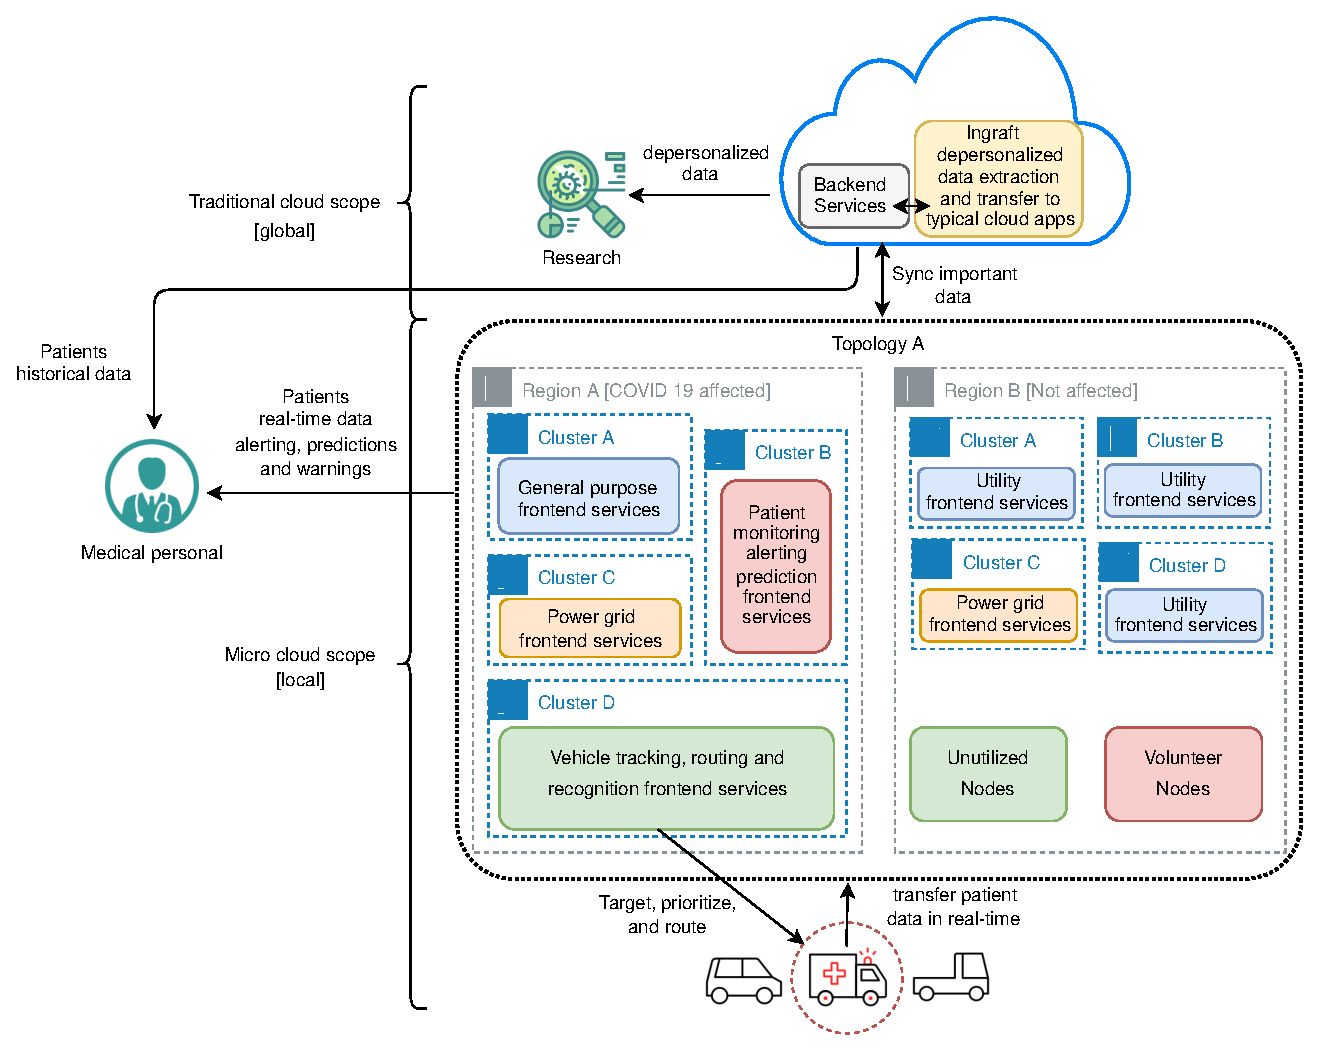
\includegraphics[width=\columnwidth]{images/Figure25}
	\end{center}
	\vspace{-0.5cm}
	\caption{Conceptual architecture model for COVID-19 area traffic control example}
	\label{fig:fig25}
\end{figure}
%
%
%!TEX root =  main.tex
\chapter{Conclusion}\label{chapter:Conclusion}
%
This chapter gives the summary of contributions for this thesis in Section~\ref{sec:summary_of_contributions}. Section~\ref{sec:limitations} presents limitations of our model, while Section~\ref{sec:future_work} presents future work.
%
%
\section{Contributions of the thesis}\label{sec:summary_of_contributions}
%
This thesis presents a possible solution to how to organize geo-distributed EC nodes into $\upmu$Cs that will be able to serve the requests of the nearby population. We have introduced an extension of $\upmu$DCs based on proven abstractions from cloud computing like zones and regions but adapted for different usage scenarios.

These easy to understand, yet powerful abstractions with slight adaptations, allowed us to cover any arbitrary vast geographic area, and yield a more available and reliable system forming the $\upmu$C model. These abstractions are easy to organize and reorganize, and $\upmu$C size is determined by the population needs descriptively. 

We have also presented the cloud to ECC mapping, showing differences between two architecture models. Furthermore, we have given a formal model of the system and its protocols used to form such a system, with clear SoC and native application model for future $\upmu$Cs infrastructure and service development. The thesis also presents a proof of concept implementation and discusses integration into existing solutions, limitation of such a system with a few applications that could be used in.

Chapter~\ref{chapter:Intro} presents the motivation for this thesis with problem are, hypothesis combined with goals and research questions this thesis is built on.

A short introduction to the topic of distributed system is given in Chapter~\ref{chapter:Field_overview}, with a short introduction to the topic of distributed systems, with a focus only on the areas that are important for the understanding of this thesis. 

It is shown what distributed systems are. We present problems these systems create, and why they are so hard to implement and maintain. It also presents a few distributed computing applications, that we can use to employ nodes in the distributed system. Further on it is shown what scalability is and why it is important for distributed systems, with few organizational ideas like peer-to-peer and membership that protocol that is important in a distributed environment for various reasons.

Virtualization techniques are then described that can be used to pack and deploy applications and infrastructure, how to implement various deployment techniques especially in the CC environment, but also the difference between DS and few models that are usually confused as distributed like parallel computing and decentralized computing.

Chapter~\ref{chapter:Review} shows related work done by various other researchers or, companies, focused again only on things that are related to this thesis.

We show different platform options, where people change the existing solutions like Kubernetes or OpenStack to made them work in areas like edge computing and mobile computing. Implementations of a few new platforms to use volunteer nodes to do some computation and storage on them with drop computing and systems like Nebula are shown further.

It is show how nodes can be organized to split some geographic area into zones, and show how $\upmu$DCs can help CC to serve requests from the local population. Different offloading techniques are used today, how to offload tasks from mobile devices closer to fog or edge nodes, but also various application models that could harness these offloading techniques and nodes organizations.

In the end, the position of this thesis, compared to other similar researches, is presented.

Chapter~\ref{chapter:Micro_clouds} presents the main contribution of this thesis. We dissect all important aspects that we need to have to help CC with latency issues, Big Data with huge volumes of data especially in the age of mobile devices and IoT.

Our model is based around $\upmu$DCs that are zonally organized, that will serve local population and population nearby. We present a model that is based on CC but adapted for different scenarios and use cases.

We show how we can dynamically form new clusters, regions, and topologies and how we can use them in the new age of mobile devices and IoT. These newly formed systems will have clear the SoC, adopted from existing research to three-tier architecture. The formed model will serve as a pre-processing layer, firewall, or privacy layers, and it is adjustable in various dimensions.

The presented model can be formed in such a way to serve larger or smaller geographic areas, where users are located. This is a matter of agreement and a matter of choice. We present how developers can use this new infrastructure and what possible models of applications could exist, and how operations can deploy developed services onto existing infrastructure.

In the end, we present the repercussions of this model, and how it can be used as an integral part of existing systems to serve as topology storage or as a new model on top of which new subsystems and applications can be developed. We present protocols for the creation of such a system and model them using asynchronous session types. The system follows a formal model, and it is easy to extend.

Finally, we give limitations of such a system and things we must be aware of.

Chapter~\ref{chapter:Implementation} presents an implemented framework that is based on knowledge compiled from previous chapters. We also present in detail operations that could be done in the framework, where it fits in the presented SoC model.

It further presents the results of our experiments in a controlled environment, what, the limitations of the framework at the current stage, and possible applications, and where this model could be used and beneficial.

The thesis is concluded in this last chapter with what  is done, what can be done in the future in form of future work.
%
%
\section{Limitations}\label{sec:limitations}
%
The model proposed in this thesis has some llimitations that we must be aware of. When talking about small-scale servers and $\upmu$Cs, we must be aware of a few things.

\begin{enumerate}[start=1,label={(\bfseries \arabic*)}]
	\item Not all organizations will be able to deploy $\upmu$Cs, due to the high initial investments required~\cite{MonsalveCC18}. We can rely on government authorities, large cloud providers, or other big companies to build the initial infrastructure for their own needs, and lease it to others similar to the cloud. The general public can use them, similarly to the cloud -- pay as you go, model;
	\item There is no guarantee that existing public cloud providers will allow nodes that are not built, resigned, or deployed by them. If we are building a private cloud, then  we can make a different decision. One way to resolve this issue is that the whole platform becomes open-source so that public cloud providers can engage in the development, and eventually use them as a solution;
	\item These small-scale servers must be out of reach of people and protected in some way so that not everyone has access to them. Some degree of physical security must be implemented;
	\item The places where these small scale servers will be deployed must have a stable internet connection, and the ability to integrate SDN or other similar technologies, so that complex network topologies could be implemented properly;
	\item These servers can have some open architecture or could be custom built by other providers. In both cases, they must be able to satisfy rules that are presented in Section~\ref{sec:separation_of_concerns};
	\item Splitting the processing into two parts and the possibility that users can be responsible for $\upmu$Cs may raise some legal concerns. Either to develop interesting applications, use them as a firewall or simply use them as a privacy level for data, there must be a legal agreement that might not be that easy to achieve.
\end{enumerate}
%
%
\subsection{Discussion}
%
The specialized infrastructure in models like~\cite{BaccarelliNSSA17, GuoRG20, JeonK19, BCAK19, ChiariniRAMG13} is required to solve a single problem. The model proposed in this thesis is more oriented towards a wider specter of applications, without the need for specialized hardware or software. Users should build applications, similarly as they build them for the cloud. Even existing applications models (e.g., microservices, serverless functions) could be transferred from cloud to $\upmu$C.

One advantage is that specialized models are developed and optimized for a specific use case taking the maximum out of existing hardware and software. Compared to the presented model (in terms of speed), in some situations, they might outperform the proposed model. On the other hand, the proposed model offers much more freedom for development (in terms of agility and applicability). This development freedom gives the users a new platform for creating interesting human-centered applications spanning over CC and $\upmu$Cs~\cite{VillariCF17}.

Specialized platforms usually require special types of applications, while the proposed model does not limit users (in terms of development tools and techniques), as long as their application could be virtualized in some way (e.g., using virtual machines, containers, or unikernels). The developers may reuse existing knowledge to develop their applications.

The proposed model allows the organization of storage and processing resources according to priority if a catastrophic event occurs (e.g., COVID-19 see section~\ref{sec:covid_example}). Providers can organize their resources and manage their digital infrastructure, where developers make applications that will help its citizens.
%
%
\section{Future work}\label{sec:future_work}
%
The work on the $\upmu$Cs is at an early stage and leaves many open questions. As a part of our current and future work, we are planning to extend the proposed model in different directions. Future work might be separated into three options:
 
\begin{enumerate}[start=1,label={(\bfseries \arabic*)}]
	\item features that operations people (eg. DevOps and SREs) users can benefit from;
	\item features developers might benefit from;
	\item infrastructure features, that both previous groups can benefit from;
\end{enumerate}

\noindent
For the first group, the first thing that should be implemented is remote cluster management, using configurations, security credentials, and actions over nodes in one or multiple clusters. On formed clusters, the users should be able to do remote configurations that nodes and/or applications can use and set up the data without going from node to node.

The system should also be extended with namespaces for usage in environments with many users in multiple teams -- multi-tenant environments. Namespaces provide the separation on virtual clusters, running on the same physical hardware. Speaking about multi-tenancy, we are also planning to implement role-based access control integrate with authentification and authorization services, with the addition of controlling different users with quotas, using rate limiting and resource limiting.

Also one possible approach would be to extend resources dynamically using infrastructure auto-scaling mechanism, so that system can grow and shrink as needed.

We are also planning to implement a full architecture and applications monitoring, alerting, and reporting that would be helpful to any administrator of such a system. We might also consider rethinking networking and making network isolation so that once formed topologies can communicate within themselves, and a possibility to specify 
strategies of communication with other topologies.

Queueing system mentioned in section~\ref{sec:queueing} should be extended so that users and/or operations people can easily add new queues and possibly assign a role for them.

We should extend the access pattern so that users can issue commands to $\upmu$Cs directly instead of going over the cloud master process only. Here we need to implement synchronization in multi-cloud deployment.

For the last part in this operations section, we should also think about continuous integration, deployment, and delivery of services onto the infrastructure, and as well as various UI dashboards that can be customized to present different aspects of the system.

Another direction for future work is the implementation which developers could benefit from. The first thing that should be implemented here is the complete application framework so that users can start developing services that can do something. We should also implement a framework and maybe domain-specific language for the use case where users just want to pre-process the data before sending it to the cloud, in a more convenient way than writing the whole application.

Users can develop their applications with different models: 

\begin{enumerate}[start=1,label={(\bfseries \arabic*)}]
	\item \textbf{mPaaS}, where the platform is doing all the management and offers a simple interface for developers to deploy their applications;
	\item \textbf{mCaaS}, if users require more control over resources requirements, deployment and orchestration decisions;
	\item \textbf{mSaaS}, users can develop their solutions only using $\upmu$Cs, but this is not advised at the moment;
\end{enumerate}

\noindent
The second would be file system and database APIs that users can use to store their data. We should also provide an interface for extensions so that others can create their databases following different models from which developers can benefit, but also integrating existing ones.

The last part of the future work be extending the current system with tunable replicating strategies for the data, in case that any part of the topology fails for whatever reason, data would not be lost. Furthermore, we should provide tunable CC synchronization models that could be used.

We should implement a scheduling system for user-developed applications so that we can put applications into the formed architecture. And last but not least, we are planning to add several security layers to protect a system in general from malicious users.

We should investigate compression methods to reduce data stored and sent via the network. These tests should be conducted on ARM devices with existing methods, or maybe we can create a ground for new compression methods and techniques.

It is stated in section~\ref{sec:repercussion} of this thesis that this model could be integrated into existing solutions. Our efforts should go as well on integrating this system with existing solutions so that they can benefit from this hierarchical and geo-distributed nodes organization in the same way or almost the same way as the stand-alone solution would.
%
%
%
%
\bibliographystyle{elsarticle-num}
\bibliography{bib}\cleardoublepage
%
%
\pagestyle{empty}
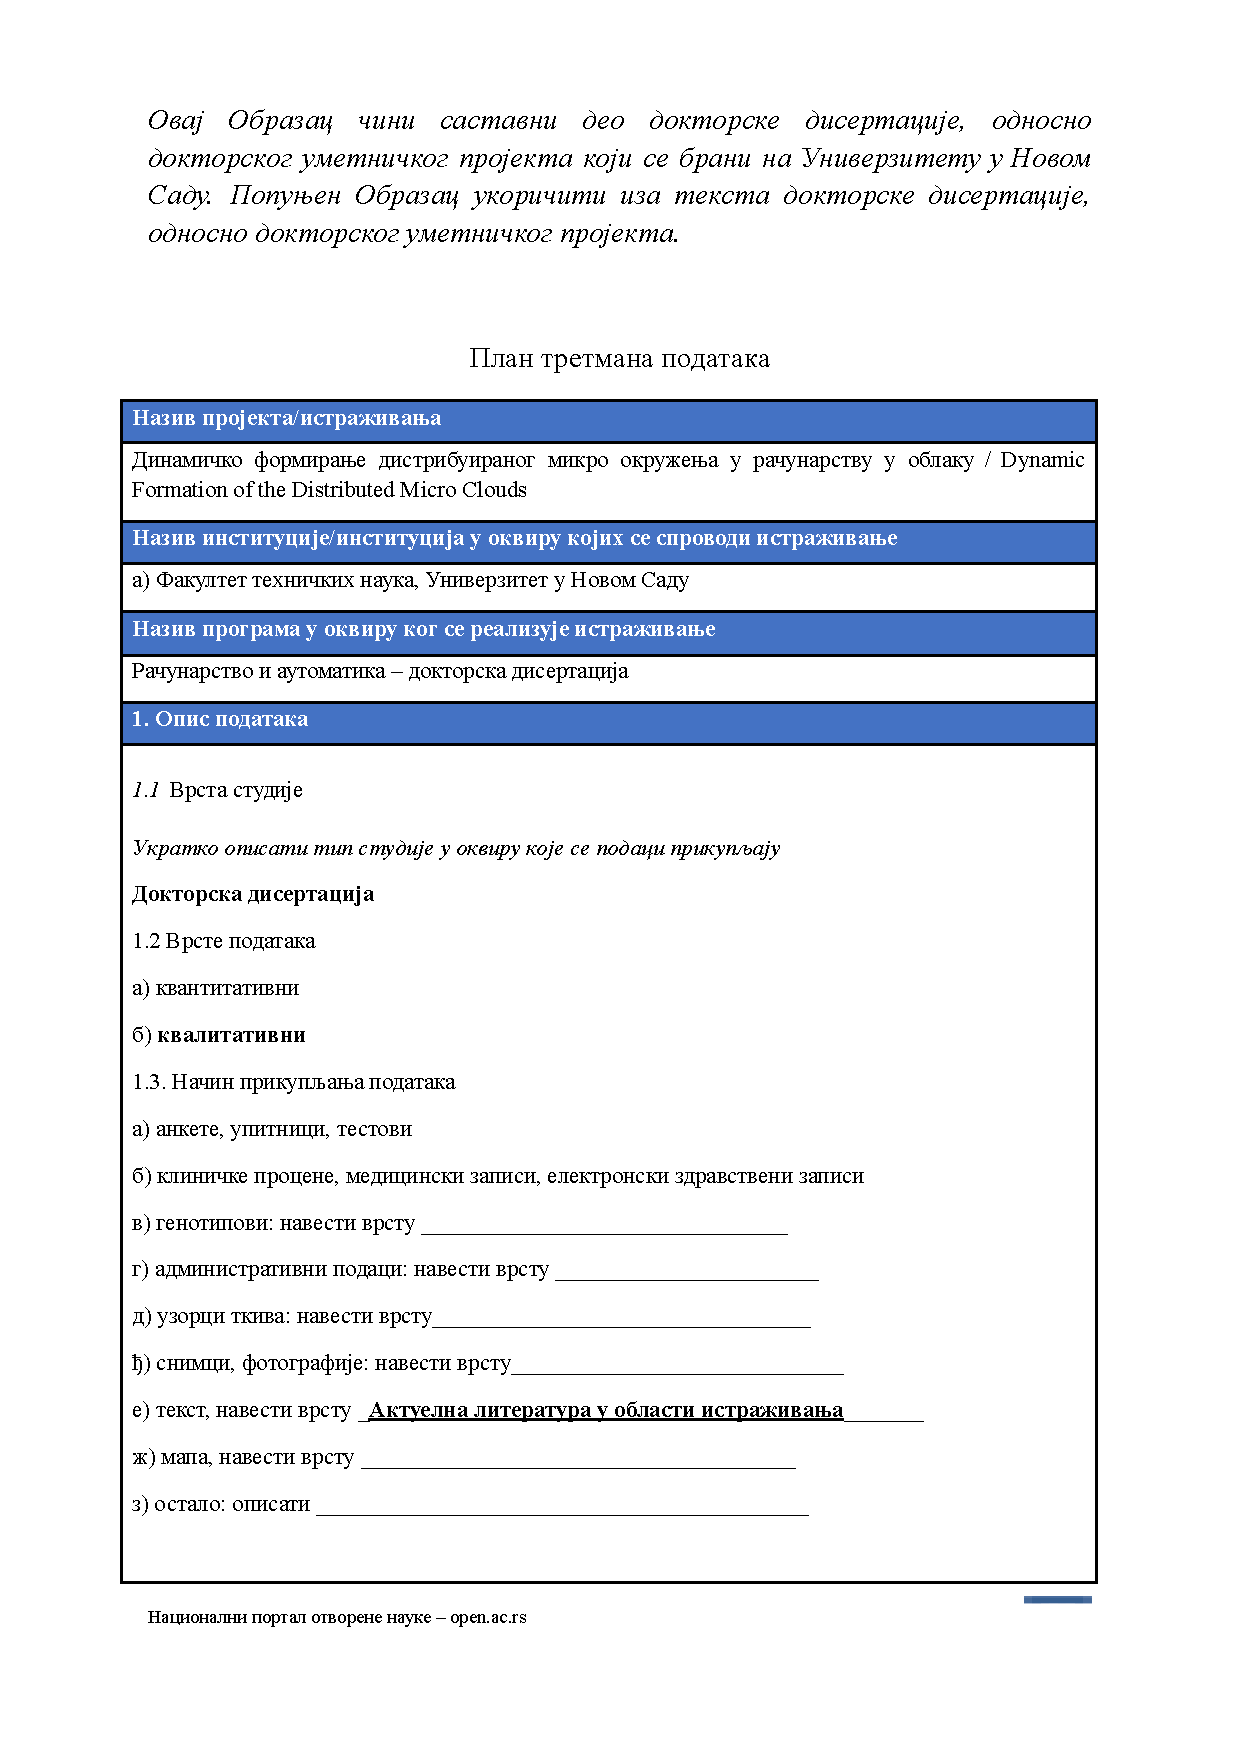
\includepdf[pages=-]{docs/plantretmanapodataka.pdf}\cleardoublepage
%
%
\pagestyle{empty}
%!TEX root =  main.tex
\chapter*{Biography}
\pagenumbering{gobble}
%\pagestyle{empty}
%
The work in this thesis is a synthesis of a few individual parts:

\begin{enumerate}[start=1,label={(\bfseries \arabic*)}]
	\item The experience acquired at a university on the topic of software engineering,
	\item The research conducted as part of the Ph.D. studies, covering various aspects of the distributed systems,
	\item The work done in collaboration with prominent software vendors,
	\item The collaboration with researchers from different research areas.
\end{enumerate}

\noindent
Milo\v s Simi\'c is a Ph.D. student and teaching assistant within the Department of Computing and Control, Faculty of Technical Sciences,  University of Novi Sad since 2015. He received his B.Sc. degree in 2014, and M.Sc. degree in 2015, all in Computer Science from the University of Novi Sad, Faculty of Technical Sciences. He is the owner of two team awards: \textbf{(1)} Best paper award \emph{(academia)}, and \textbf{(2)} ThinkX in the category Community and Social Impact \emph{(industry)}.\\\\
\noindent
Over the years, Milo\v s worked with various prominent software vendors, in different fields. This allowed him to combine the different skillsets developed over the years and focus his expertise towards designing and implementing distributed and non-distributed software systems, for various usages. His research interests include: \textbf{(1)} distributed systems, \textbf{(2)} (multi) cloud computing, \textbf{(3)} edge computing, \textbf{(4)} NoSQL engines and big data, and \textbf{(5)} service-oriented architectures and microservices.\\\\
\noindent
As part of his Ph.D., Milo\v s has studied different distributed systems techniques, combined with various software engineering methodologies and practices covering both standard-defined processes and industry-proven methods, to solve and answer such complicated questions that are part of this thesis. The chance to work with different software vendors and combine that knowledge with traditional academic approaches, helped Miloš to determine what are the main research questions that need to be answered and guided him to the work that is described in this thesis.\\\\
\noindent
Through collaboration with people from different research areas, this thesis is enriched with formal description and formal model that are important leverage to describe and validate such a complicated system. The efforts put into this research resulted in reaching only the tip of the iceberg of future opportunities. In 2021, the portion of the work that was published in the IEEE Access journal (paper cf. journal paper~\ref{accessSimic}) was presented to the eminent professors and colleagues from the \emph{Imperial College London}, as an invited lecture.\\\\

\noindent
Further challenges are yet to come.
%
%\cleardoublepage
%
%
%!TEX root =  main.tex
\chapter*{List of publications}
\pagenumbering{gobble}
%
This thesis is the result based on the previously papers presented on conferences and journals.

\begin{enumerate}
	\item M. Simić, I. Prokić, J. Dedeić, G. Sladić and B. Milosavljević, "Towards Edge Computing as a Service: Dynamic Formation of the Micro Data-Centers," in IEEE Access, vol. 9, pp. 114468-114484, 2021, doi: 10.1109/ACCESS.2021.3104475.
	\item Simić, M., Stojkov, M., Sladić, G., Milosavljević, B.  CRDTs as replication strategy in large-scale edge distributed system: An overview. In: Zdravković, M., Konjović, Z., Trajanović, M. (Eds.) ICIST 2020 Proceedings Vol.1, pp.46-50, 2020, ISBN 978-86-85525-24-7.
	\item Simić M., Stojkov M., Sladić G., Milosavljević B., Zarić M.:   On container usability in large-scale edge distributed system, 9. International Conference on Information Science and Technology (ICIST), Kopaonik: Society for Information Systems and Computer Networks, 10-13 March, 2019, pp. 97-101, ISBN pp.97-101, 2019.
	\item Simić M., Stojkov M., Sladić G., Milosavljević B.:  Edge computing system for large-scale distributed sensing systems, 8. International Conference on Information Science and Technology (ICIST), Kopaonik: Society for Information Systems and Computer Networks, 11-14 March, 2018, pp. 36-39, ISBN 978-86-85525-22-3.
	\item Simić M., Sladić G., Milosavljević B.:  A Case Study IoT and Blockchain Powered Healthcare , 8. PSU-UNS International Conference on Engineering and Technology - ICET, Novi Sad: University of Novi Sad, Faculty of Technical Sciences , 8-10 June, 2017, pp. 1-4, ISBN 978-86-7892-934-2.
\end{enumerate}
%
%\cleardoublepage
%
%
\end{document}